%------------------------------------------------------------------------------------
%	Pacotes e Outras Configurações
%------------------------------------------------------------------------------------
\documentclass[a4paper,11pt]{book} % Fonte do livro
%----------------------------------------------------------------------------------
% The Legrand Orange Book
% Structural Definitions File
% Version 2.0 (9/2/15)
%----------------------------------------------------------------------------------
% \documentclass[a4paper,11pt]{book} % Fonte do livro

%----------------------------------------------------------------------------------
%	VARIOUS REQUIRED PACKAGES AND CONFIGURATIONS
%----------------------------------------------------------------------------------
\usepackage[top=3cm,bottom=3cm,left=3cm,right=2cm,headsep=10pt,a4paper]{geometry} % Page margins
\usepackage{import}
\usepackage{lipsum} % Inserts dummy text
\usepackage[brazil]{babel} % Brazil language/hyphenation
\usepackage{graphicx} % Required for including pictures
\usepackage{wrapfig} % Imagens que se cruzam com texto
\usepackage{tikz} % Required for drawing custom shapes
\usepackage[T1]{fontenc}
\usepackage[utf8]{inputenc} % Required for including letters with accents
\usepackage{enumitem} % Customize lists
\usepackage{longtable}
\usepackage{booktabs} % Required for nicer horizontal rules in tables
\usepackage{xcolor} % Required for specifying colors by name
\usepackage{listings} % listagens
\usepackage{float}
%----------------------------------------------------------------------------------
%	IMAGENS
%----------------------------------------------------------------------------------
\graphicspath{{Pictures/}} % Specifies the directory where pictures are stored
%----------------------------------------------------------------------------------
%	CAIXA DE LISTAGEM
%----------------------------------------------------------------------------------
\definecolor{ocre}{RGB}{243,102,25} % Define the orange color used for highlighting throughout the book
% Definição para as caixas de listagens
\definecolor{codegray}{rgb}{0.5,0.5,0.5}
\definecolor{backcolour}{rgb}{0.95,0.95,0.92}

% Espaçamento dos Parágrafos
\setlength{\parindent}{0em}
\setlength{\parskip}{1em}

\lstset {
 aboveskip=3mm,
 backgroundcolor=\color{backcolour},
 basicstyle={\small\ttfamily},
 belowskip=3mm,
 breaklines=true,
 breakatwhitespace=true,
 columns=flexible,
 commentstyle=\textit,
 frame=tb,
 keepspaces=true,
 keywordstyle=\color{blue}\bfseries,
 % language=Java, Python, HTML, CSS
 showstringspaces=false,
 showtabs=false,
 tabsize=3
}
%----------------------------------------------------------------------------------
%	FONTS
%----------------------------------------------------------------------------------
\usepackage{avant} % Use the Avantgarde font for headings
\usepackage{mathptmx} % Use the Adobe Times Roman as the default text font together
\usepackage{microtype} % Slightly tweak font spacing for aesthetics
\usepackage[T1]{fontenc} % Use 8-bit encoding that has 256 glyphs
%----------------------------------------------------------------------------------
%	BIBLIOGRAPHY AND INDEX
%----------------------------------------------------------------------------------
% \usepackage[style=numeric,citestyle=numeric,sorting=nyt,sortcites=true,autopunct=true,hyperref=true,abbreviate=false,backref=true,backend=biber]{biblatex}
%\addbibresource{bibliography.bib} % BibTeX bibliography file
% \defbibheading{bibempty}{}
\usepackage{calc} % For simpler calculation - used for spacing the index letter headings correctly
\usepackage{makeidx} % Required to make an index
\makeindex % Tells LaTeX to create the files required for indexing
%----------------------------------------------------------------------------------
%	MAIN TABLE OF CONTENTS
%----------------------------------------------------------------------------------
\usepackage{titletoc} % Required for manipulating the table of contents
\contentsmargin{0cm} % Removes the default margin
% Part text styling
\titlecontents{part}[0cm]
{\addvspace{20pt}\centering\large\bfseries}
{}
{}
{}
% Chapter text styling
\titlecontents{chapter}[1.25cm] % Indentation
{\addvspace{12pt}\large\sffamily\bfseries} % Spacing and font options for chapters
{\color{ocre!60}\contentslabel[\Large\thecontentslabel]{1.25cm}\color{ocre}} % Chapter number
{\color{ocre}}  
{\color{ocre!60}\normalsize\;\titlerule*[.5pc]{.}\;\thecontentspage} % Page number
% Section text styling
\titlecontents{section}[1.25cm] % Indentation
{\addvspace{3pt}\sffamily\bfseries} % Spacing and font options for sections
{\contentslabel[\thecontentslabel]{1.25cm}} % Section number
{}
{\hfill\color{black}\thecontentspage} % Page number
[]
% Subsection text styling
\titlecontents{subsection}[1.25cm] % Indentation
{\addvspace{1pt}\sffamily\small} % Spacing and font options for subsections
{\contentslabel[\thecontentslabel]{1.25cm}} % Subsection number
{}
{\ \titlerule*[.5pc]{.}\;\thecontentspage} % Page number
[]
% List of figures
\titlecontents{figure}[0em]
{\addvspace{-5pt}\sffamily}
{\thecontentslabel\hspace*{1em}}
{}
{\ \titlerule*[.5pc]{.}\;\thecontentspage}
[]
% List of tables
\titlecontents{table}[0em]
{\addvspace{-5pt}\sffamily}
{\thecontentslabel\hspace*{1em}}
{}
{\ \titlerule*[.5pc]{.}\;\thecontentspage}
[]
%----------------------------------------------------------------------------------
%	MINI TABLE OF CONTENTS IN PART HEADS
%----------------------------------------------------------------------------------
% Chapter text styling
\titlecontents{lchapter}[0em] % Indenting
{\addvspace{15pt}\large\sffamily\bfseries} % Spacing and font options for chapters
{\color{ocre}\contentslabel[\Large\thecontentslabel]{1.25cm}\color{ocre}} % Chapter number
{}  
{\color{ocre}\normalsize\sffamily\bfseries\;\titlerule*[.5pc]{.}\;\thecontentspage} % Page number
% Section text styling
\titlecontents{lsection}[0em] % Indenting
{\sffamily\small} % Spacing and font options for sections
{\contentslabel[\thecontentslabel]{1.25cm}} % Section number
{}
{}
% Subsection text styling
\titlecontents{lsubsection}[.5em] % Indentation
{\normalfont\footnotesize\sffamily} % Font settings
{}
{}
{}
%----------------------------------------------------------------------------------
%	PAGE HEADERS
%----------------------------------------------------------------------------------
\usepackage{fancyhdr} % Required for header and footer configuration
\pagestyle{fancy}
\renewcommand{\chaptermark}[1]{\markboth{\sffamily\normalsize\bfseries\chaptername\ \thechapter.\ #1}{}} % Chapter text font settings
\renewcommand{\sectionmark}[1]{\markright{\sffamily\normalsize\thesection\hspace{5pt}#1}{}} % Section text font settings
\fancyhf{} \fancyhead[LE,RO]{\sffamily\normalsize\thepage} % Font setting for the page number in the header
\fancyhead[LO]{\rightmark} % Print the nearest section name on the left side of odd pages
\fancyhead[RE]{\leftmark} % Print the current chapter name on the right side of even pages
\renewcommand{\headrulewidth}{0.5pt} % Width of the rule under the header
\addtolength{\headheight}{12pt} % Increase the spacing around the header slightly
\renewcommand{\footrulewidth}{0pt} % Removes the rule in the footer
\fancypagestyle{plain}{\fancyhead{}\renewcommand{\headrulewidth}{0pt}} % Style for when a plain pagestyle is specified
% Removes the header from odd empty pages at the end of chapters
\makeatletter
\renewcommand{\cleardoublepage}{
    \ifodd\c@page\else
    \hbox{}
    \vspace*{\fill}
    \thispagestyle{empty}
    \newpage
    \fi
}
%----------------------------------------------------------------------------------
%	THEOREM STYLES
%----------------------------------------------------------------------------------
\usepackage{amsmath,amsfonts,amssymb,amsthm} % For math equations, theorems, symbols, etc
\newcommand{\intoo}[2]{\mathopen{]}#1\,;#2\mathclose{[}}
\newcommand{\ud}{\mathop{\mathrm{{}d}}\mathopen{}}
\newcommand{\intff}[2]{\mathopen{[}#1\,;#2\mathclose{]}}
\newtheorem{notation}{Anotação}[chapter]
% Boxed/framed environments
\newtheoremstyle{ocrenumbox}% % Theorem style name
{10pt}% Space above
{0pt}% Space below
{\normalfont}% % Body font
{}% Indent amount
{\small\bf\sffamily\color{ocre}}% % Theorem head font
{\;}% Punctuation after theorem head
{0.25em}% Space after theorem head
{\small\sffamily\color{ocre}\thmname{#1}\nobreakspace\thmnumber{\@ifnotempty{#1}{}\@upn{#2}}% Theorem text (e.g. Theorem 2.1)
\thmnote{\nobreakspace\the\thm@notefont\sffamily\bfseries\color{black}---\nobreakspace#3.}} % Optional theorem note
\renewcommand{\qedsymbol}{$\blacksquare$}% Optional qed square
% Boxed/framed environments
\newtheoremstyle{blacknumex}% Theorem style name
{5pt}% Space above
{5pt}% Space below
{\normalfont}% Body font
{} % Indent amount
{\small\bf\sffamily}% Theorem head font
{\;}% Punctuation after theorem head
{0.25em}% Space after theorem head
{\small\sffamily{\tiny\ensuremath{\blacksquare}}\nobreakspace\thmname{#1}\nobreakspace\thmnumber{\@ifnotempty{#1}{}\@upn{#2}}% Theorem text (e.g. Theorem 2.1)
\thmnote{\nobreakspace\the\thm@notefont\sffamily\bfseries---\nobreakspace#3.}}% Optional theorem note
% Boxed/framed environments
\newtheoremstyle{blacknumbox} % Theorem style name
{0pt}% Space above
{0pt}% Space below
{\normalfont}% Body font
{}% Indent amount
{\small\bf\sffamily}% Theorem head font
{\;}% Punctuation after theorem head
{0.25em}% Space after theorem head
{\small\sffamily\thmname{#1}\nobreakspace\thmnumber{\@ifnotempty{#1}{}\@upn{#2}}% Theorem text (e.g. Theorem 2.1)
\thmnote{\nobreakspace\the\thm@notefont\sffamily\bfseries---\nobreakspace#3.}}% Optional theorem note
% Non-boxed/non-framed environments
\newtheoremstyle{ocrenum}% % Theorem style name
{5pt}% Space above
{5pt}% Space below
{\normalfont}% % Body font
{}% Indent amount
{\small\bf\sffamily\color{ocre}}% % Theorem head font
{\;}% Punctuation after theorem head
{0.25em}% Space after theorem head
{\small\sffamily\color{ocre}\thmname{#1}\nobreakspace\thmnumber{\@ifnotempty{#1}{}\@upn{#2}}% Theorem text (e.g. Theorem 2.1)
\thmnote{\nobreakspace\the\thm@notefont\sffamily\bfseries\color{black}---\nobreakspace#3.}} % Optional theorem note
\renewcommand{\qedsymbol}{$\blacksquare$}% Optional qed square
\makeatother
% Defines the theorem text style for each type of theorem to one of the three styles above
\newcounter{dummy} 
\numberwithin{dummy}{section}
\theoremstyle{ocrenumbox}
\newtheorem{theoremeT}{Observação}
\newtheorem{problem}{Problema}[chapter]
\newtheorem{exerciseT}{Exercício}[chapter]
\theoremstyle{blacknumex}
\newtheorem{exampleT}{Exemplo}[chapter]
\theoremstyle{blacknumbox}
\newtheorem{vocabulary}{Vocabulário}[chapter]
\newtheorem{definitionT}{Definição}[section]
\newtheorem{dicaT}{Dica}
\theoremstyle{ocrenum}
\newtheorem{proposition}[dummy]{Proposition}
%------------------------------------------------------------------------------------
%	DEFINITION OF COLORED BOXES
%------------------------------------------------------------------------------------
\RequirePackage[framemethod=default]{mdframed} % Required for creating the theorem, definition, exercise and dica boxes
% Theorem box
\newmdenv[skipabove=7pt,
    skipbelow=7pt,
    backgroundcolor=black!5,
    linecolor=ocre,
    innerleftmargin=5pt,
    innerrightmargin=5pt,
    innertopmargin=5pt,
    leftmargin=0cm,
    rightmargin=0cm,
    innerbottommargin=5pt]{tBox}
% Exercise box	  
\newmdenv[skipabove=7pt,
    skipbelow=7pt,
    rightline=false,
    leftline=true,
    topline=false,
    bottomline=false,
    backgroundcolor=ocre!10,
    linecolor=ocre,
    innerleftmargin=5pt,
    innerrightmargin=5pt,
    innertopmargin=5pt,
    innerbottommargin=5pt,
    leftmargin=0cm,
    rightmargin=0cm,
    linewidth=4pt]{eBox}	
% Definition box
\newmdenv[skipabove=7pt,
    skipbelow=7pt,
    rightline=false,
    leftline=true,
    topline=false,
    bottomline=false,
    linecolor=ocre,
    innerleftmargin=5pt,
    innerrightmargin=5pt,
    innertopmargin=0pt,
    leftmargin=0cm,
    rightmargin=0cm,
    linewidth=4pt,
    innerbottommargin=0pt]{dBox}	
% Caixa de Dica
\newmdenv[skipabove=7pt,
    skipbelow=7pt,
    rightline=false,
    leftline=true,
    topline=false,
    bottomline=false,
    linecolor=gray,
    backgroundcolor=black!5,
    innerleftmargin=5pt,
    innerrightmargin=5pt,
    innertopmargin=5pt,
    leftmargin=0cm,
    rightmargin=0cm,
    linewidth=4pt,
    innerbottommargin=5pt]{cBox}
% Creates an environment for each type of theorem and assigns it a theorem text style 
% from the Theorem Styles section above and a colored box from above
\newenvironment{theorem}{\begin{tBox}\begin{theoremeT}}{\end{theoremeT}\end{tBox}}
\newenvironment{exercise}{\begin{eBox}\begin{exerciseT}}{\hfill{\color{ocre}\tiny\ensuremath{\blacksquare}}\end{exerciseT}\end{eBox}}
\newenvironment{definition}{\begin{dBox}\begin{definitionT}}{\end{definitionT}\end{dBox}}	
\newenvironment{example}{\begin{exampleT}}{\hfill{\tiny\ensuremath{\blacksquare}}\end{exampleT}}
\newenvironment{dica}{\begin{cBox}\begin{dicaT}}{\end{dicaT}\end{cBox}}
%------------------------------------------------------------------------------------
%	REMARK ENVIRONMENT
%------------------------------------------------------------------------------------
\newenvironment{remark}{\par\vspace{10pt}\small % Vertical white space above the remark and smaller font size
\begin{list}{}{
    \leftmargin=35pt % Indentation on the left
    \rightmargin=25pt}\item\ignorespaces % Indentation on the right
\makebox[-2.5pt]{\begin{tikzpicture}[overlay]
    \node[draw=ocre!60,line width=1pt,circle,fill=ocre!25,font=\sffamily\bfseries,inner sep=2pt,outer sep=0pt] at (-15pt,0pt){\textcolor{ocre}{F}};\end{tikzpicture}} % Orange R in a circle
    \advance\baselineskip -1pt}{\end{list}\vskip5pt} % Tighter line spacing and white space after remark
%------------------------------------------------------------------------------------
%	SECTION NUMBERING IN THE MARGIN
%------------------------------------------------------------------------------------
\makeatletter
\renewcommand{\@seccntformat}[1]{\llap{\textcolor{ocre}{\csname the#1\endcsname}\hspace{1em}}}                    
\renewcommand{\section}{\@startsection{section}{1}{\z@}
    {-4ex \@plus -1ex \@minus -.4ex}
    {1ex \@plus.2ex }
    {\normalfont\large\sffamily\bfseries}}
\renewcommand{\subsection}{\@startsection {subsection}{2}{\z@}
    {-3ex \@plus -0.1ex \@minus -.4ex}
    {0.5ex \@plus.2ex }
    {\normalfont\sffamily\bfseries}}
\renewcommand{\subsubsection}{\@startsection {subsubsection}{3}{\z@}
    {-2ex \@plus -0.1ex \@minus -.2ex}
    {.2ex \@plus.2ex }
    {\normalfont\small\sffamily\bfseries}} 
\renewcommand\paragraph{\@startsection{paragraph}{4}{\z@}
    {-2ex \@plus-.2ex \@minus .2ex}
    {.1ex}
    {\normalfont\small\sffamily\bfseries}}
%------------------------------------------------------------------------------------
%	PART HEADINGS
%------------------------------------------------------------------------------------
% numbered part in the table of contents
\newcommand{\@mypartnumtocformat}[2]{
    \setlength\fboxsep{0pt}
    \noindent\colorbox{ocre!20}{\strut\parbox[c][.7cm]{\ecart}{\color{ocre!70}\Large\sffamily\bfseries\centering#1}}\hskip\esp\colorbox{ocre!40}{\strut\parbox[c][.7cm]{\linewidth-\ecart-\esp}{\Large\sffamily\centering#2}}}
% unnumbered part in the table of contents
\newcommand{\@myparttocformat}[1]{
    \setlength\fboxsep{0pt}
    \noindent\colorbox{ocre!40}{\strut\parbox[c][.7cm]{\linewidth}{\Large\sffamily\centering#1}}}
\newlength\esp
\setlength\esp{4pt}
\newlength\ecart
\setlength\ecart{1.2cm-\esp}
\newcommand{\thepartimage}{}
\newcommand{\partimage}[1]{\renewcommand{\thepartimage}{#1}}
\def\@part[#1]#2{
    \ifnum \c@secnumdepth >-2\relax
        \refstepcounter{part}
        \addcontentsline{toc}{part}{\texorpdfstring{\protect\@mypartnumtocformat{\thepart}{#1}}{\partname~\thepart\ ---\ #1}}
    \else
        \addcontentsline{toc}{part}{\texorpdfstring{\protect\@myparttocformat{#1}}{#1}}
    \fi
    \startcontents
    \markboth{}{}
    {\thispagestyle{empty}
    \begin{tikzpicture}[remember picture,overlay]
    \node at (current page.north west){\begin{tikzpicture}[remember picture,overlay]
    \fill[ocre!20](0cm,0cm) rectangle (\paperwidth,-\paperheight);
    \node[anchor=north] at (4cm,-3.25cm){\color{ocre!40}\fontsize{220}{100}\sffamily\bfseries\thepart}; 
    \node[anchor=south east] at (\paperwidth-1cm,-\paperheight+1cm){\parbox[t][][t]{8.5cm}{
    \printcontents{l}{0}{\setcounter{tocdepth}{1}}
    }};
    \node[anchor=north east] at (\paperwidth-1.5cm,-3.25cm){\parbox[t][][t]{15cm}{\strut\raggedleft\color{white}\fontsize{30}{30}\sffamily\bfseries#2}};
    \end{tikzpicture}};
    \end{tikzpicture}}
    \@endpart}
\def\@spart#1{
\startcontents
\phantomsection
{\thispagestyle{empty}
\begin{tikzpicture}[remember picture,overlay]
\node at (current page.north west){\begin{tikzpicture}[remember picture,overlay]
    \fill[ocre!20](0cm,0cm) rectangle (\paperwidth,-\paperheight);
    \node[anchor=north east] at (\paperwidth-1.5cm,-3.25cm){\parbox[t][][t]{15cm}{\strut\raggedleft\color{white}\fontsize{30}{30}\sffamily\bfseries#1}};
    \end{tikzpicture}};
\end{tikzpicture}}
\addcontentsline{toc}{part}{\texorpdfstring{
    \setlength\fboxsep{0pt}
    \noindent\protect\colorbox{ocre!40}{\strut\protect\parbox[c][.7cm]{\linewidth}{\Large\sffamily\protect\centering #1\quad\mbox{}}}}{#1}}
    \@endpart}
\def\@endpart{\vfil\newpage
    \if@twoside
        \if@openright
            \null
            \thispagestyle{empty}
            \newpage
        \fi
    \fi
    \if@tempswa
    \twocolumn
    \fi}
%------------------------------------------------------------------------------------
%	CHAPTER HEADINGS
%------------------------------------------------------------------------------------
% A switch to conditionally include a picture, implemented by  Christian Hupfer
\newif\ifusechapterimage
\usechapterimagetrue
\newcommand{\thechapterimage}{}
\newcommand{\chapterimage}[1]{\ifusechapterimage\renewcommand{\thechapterimage}{#1}\fi}
\newcommand{\autodot}{.}
\def\@makechapterhead#1{
    {\parindent \z@ \raggedright \normalfont
    \ifnum \c@secnumdepth >\m@ne
    \if@mainmatter
    \begin{tikzpicture}[remember picture,overlay]
    \node at (current page.north west)
    {\begin{tikzpicture}[remember picture,overlay]
    \node[anchor=north west,inner sep=0pt] at (0,0) {\ifusechapterimage\includegraphics[width=\paperwidth]{\thechapterimage}\fi};
    \draw[anchor=west] (\Gm@lmargin,-9cm) node [line width=2pt,rounded corners=15pt,draw=ocre,fill=white,fill opacity=0.5,inner sep=15pt]{\strut\makebox[22cm]{}};
    \draw[anchor=west] (\Gm@lmargin+.3cm,-9cm) node {\huge\sffamily\bfseries\color{black}\thechapter\autodot~#1\strut};
    \end{tikzpicture}};
    \end{tikzpicture}
    \else
    \begin{tikzpicture}[remember picture,overlay]
    \node at (current page.north west)
    {\begin{tikzpicture}[remember picture,overlay]
    \node[anchor=north west,inner sep=0pt] at (0,0) {\ifusechapterimage\includegraphics[width=\paperwidth]{\thechapterimage}\fi};
    \draw[anchor=west] (\Gm@lmargin,-9cm) node [line width=2pt,rounded corners=15pt,draw=ocre,fill=white,fill opacity=0.5,inner sep=15pt]{\strut\makebox[22cm]{}};
    \draw[anchor=west] (\Gm@lmargin+.3cm,-9cm) node {\huge\sffamily\bfseries\color{black}#1\strut};
    \end{tikzpicture}};
    \end{tikzpicture}
    \fi\fi\par\vspace*{270\p@}}}
\def\@makeschapterhead#1{
\begin{tikzpicture}[remember picture,overlay]
    \node at (current page.north west)
    {\begin{tikzpicture}[remember picture,overlay]
        \node[anchor=north west,inner sep=0pt] at (0,0) {\ifusechapterimage\includegraphics[width=\paperwidth]{\thechapterimage}\fi};
        \draw[anchor=west] (\Gm@lmargin,-9cm) node [line width=2pt,rounded corners=15pt,draw=ocre,fill=white,fill opacity=0.5,inner sep=15pt]{\strut\makebox[22cm]{}};
        \draw[anchor=west] (\Gm@lmargin+.3cm,-9cm) node {\huge\sffamily\bfseries\color{black}#1\strut};
    \end{tikzpicture}};
\end{tikzpicture}
\par\vspace*{270\p@}}
\makeatother
%------------------------------------------------------------------------------------
%	HYPERLINKS IN THE DOCUMENTS
%------------------------------------------------------------------------------------
\usepackage{url}
\usepackage{bookmark}
\bookmarksetup{
    open,
    numbered,
    addtohook={
        \ifnum\bookmarkget{level}=0 % chapter
        \bookmarksetup{bold}%
        \fi
        \ifnum\bookmarkget{level}=-1 % part
        \bookmarksetup{color=ocre,bold}
        \fi
    }
}

\raggedbottom

%------------------------------------------------------------------------------------
% A comentar
%------------------------------------------------------------------------------------
% \begin{document}
%  XPTO
% \end{document}
 % Arquivo de Pacotes e comandos

\begin{document}

%------------------------------------------------------------------------------------
%	TITLE PAGE
%------------------------------------------------------------------------------------
\begingroup
\thispagestyle{empty}
\begin{tikzpicture}[remember picture,overlay]
\node[inner sep=0pt] (background) at (current page.center) {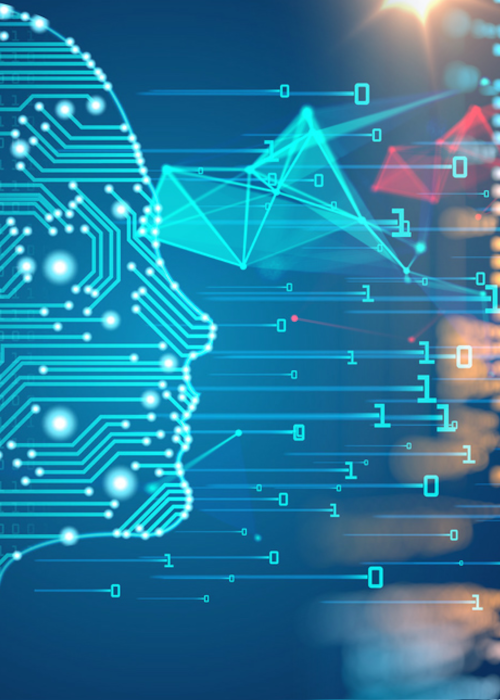
\includegraphics[width=\paperwidth]{CpFrente}};
\draw (current page.center) node [fill=ocre!30!white,fill opacity=0.6,text opacity=1,inner sep=1cm]{\Huge\centering\bfseries\sffamily\parbox[c][][t]{\paperwidth}{\centering Machine Learning na Prática\\[15pt] % Titulo
{\Large Modelos em Python}\\[20pt] % Subtitulo
{\huge Fernando Anselmo}}}; % Nome
\end{tikzpicture}
\vfill
\endgroup

%------------------------------------------------------------------------------------
%	COPYRIGHT PAGE
%------------------------------------------------------------------------------------
\newpage
~\vfill
\thispagestyle{empty}

\noindent Copyright \copyright\ 2020 Fernando Anselmo - v1.0 % Copyright

\noindent \textsc{Publicação Independente} % Publicado por

\noindent \url{http:\\fernandoanselmo.orgfree.com} % URL

\noindent \\ É permitido a total distribuição, cópia e compartilhamento deste arquivo, desde que se preserve os seguintes direitos, conforme a licença da \textit{Creative Commons 3.0}. Logos, ícones e outros itens inseridos nesta obra, são de responsabilidade de seus proprietários. Não possuo a menor intenção em me apropriar da autoria de nenhum artigo de terceiros. Caso não tenha citado a fonte correta de algum texto que coloquei em qualquer seção, basta me enviar um e-mail que farei as devidas retratações, algumas partes podem ter sido cópias (ou baseadas na ideia) de artigos que li na Internet e que me ajudaram a esclarecer muitas dúvidas, considere este como um documento de pesquisa que resolvi compartilhar para ajudar os outros usuários e não é minha intenção tomar crédito de terceiros. % License information

%------------------------------------------------------------------------------------
%	SUMARIO
%------------------------------------------------------------------------------------

% Para nao usar imagem nos capitulos
% \usechapterimagefalse 

\chapterimage{headMontagem.png} % Imagem
\pagestyle{empty} % Sem Cabecalho
\tableofcontents % Mostra a tabela de conteudo
\cleardoublepage % Forca que a primeira pagina seja iniciada em um numero impar
\pagestyle{fancy} % Volta a imprimir o Cabecalho
\clearpage % Forca que a primeira pagina seja iniciada em um numero impar

%------------------------------------------------------------------------------------
%	PARTES
%------------------------------------------------------------------------------------

%\part{Parte Um - O Básico}
% Entendimento Geral
%------------------------------------------------------------------------------------
%	CHAPTER 1
%------------------------------------------------------------------------------------
\chapterimage{headMontagem.png}
\chapter{Entendimento Geral}

\begin{remark}
Machine Learning é a habilidade de localizar padrões em Dados. (Gil Weinberg - Founding Director of Georgia Tech Center for Music Technology) 
\end{remark}

\section{Do que trata esse livro?}\index{Entendimento Geral}
Cada vez que leio um livro de \textbf{Machine Learning} tenho a sensação que o autor quer mostrar para seus leitores o quanto ele é um bom Matemático, coloca um monte de fórmulas com demonstrações (muitas delas parecem escritas em grego e usam inclusive letras gregas) é isso me faz pensar: \textit{Será que quando indicar um livro para meus alunos vou querer que eles aprendam fórmulas ou que tenham uma base em que possam praticar?} 

E graças a isso publiquei uma série de artigos sobre os mais variados modelos de \textit{Machine Learning} na rede \textbf{Linkedin} e esses artigos foram a base para esse livro, não espere encontrar aqui muitos conceitos, apesar de ser obrigado a abordá-los ou muita coisa se perderia, mas a ideia aqui é ser totalmente prático.

Já ouvimos isso de prático tantas vezes, existe duas séries de livros especialistas denominadas: "\textit{Hands On}" e "\textit{Cookbook}". Aprecio e tenho muitos desses livros, porém sempre que desejo algo no primeiro caso é muito difícil encontrar bem separado e exposto da forma como queria e no segundo está fragmentado demais. O prático aqui será: Um modelo em linguagem Python, ler bases de dados, com o uso de suas possibilidades, seu treino e melhor forma de obter resultados. Sendo assim não espere encontrar nesse aulas básicas de Python.

\section{O que é Machine Learning?}\index{Entendimento Geral}
De forma bastante genérica, algorítimos de \textit{Machine Learning} (Aprendizado de Máquina e doravante apenas \textbf{ML}) são uma mudança de paradigma da “programação tradicional” onde precisamos passar toda a heurística explicitamente para um novo conceito, onde ao invés de escrever cada ação que o algorítimos deve realizar, apenas passamos diversos exemplos e deixamos que o computador resolva (ou aprenda) quais são as “melhores” (menor custo) decisões. É também chamada de \textit{Statistical Learning} (Autores Hastie, Tibshirani \& Friedman 2009) utilizada para extrair um modelo a partir de um sistema de observações ou medidas. Sendo um campo relativamente novo da ciência composto de uma variedade de métodos (algoritmos) computacionais e estatísticos que competem entre si.
\begin{figure}[H]
	\centering
	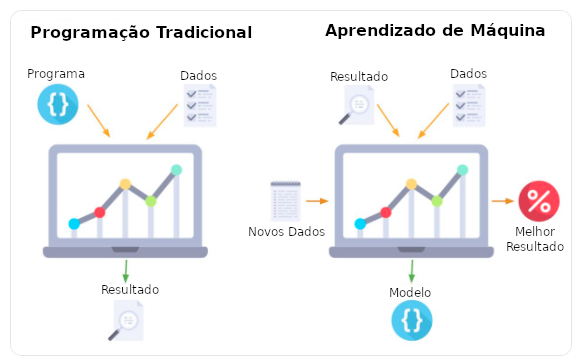
\includegraphics[width=0.7\textwidth]{cap01/EstruturaML.png}
	\caption{Programação Tradicional X Machine Learning}
\end{figure}

Ou seja, treinamos com dados e resultados anteriores até que possam receber \textbf{novos dados} e transforme isso em resultados sem que sejam explicitamente programáveis, isso é chamado de ``Modelo de ML''. Interpretar esses modelos é entender como podemos transformar algo. Em geral são classificados em:
\begin{itemize}[noitemsep]
	\item \textbf{Clusterização}: Encontrar uma estrutura de dados, sumarização.
	\item \textbf{Regressão e Estimação}: Predição de valores contínuos.
	\item \textbf{Classificação}: Predição de um item de um caso de classe/categoria.
	\item \textbf{Associação}: frequentemente ocorre entre itens e eventos.
\end{itemize}

É muito importante conhecer vários deles para decidir qual se ajusta e trabalha melhor aos dados que temos para treiná-los. Devemos ter em mente que ML pode ser bem diferente de \textbf{Estatística}. Aqui não estamos preocupados com inferência, causalidade e exogeneidade. ML está preocupada, quase que exclusivamente em melhorar as predições ou rapidamente localizar em um mar de informações aquela que buscamos. 

Assim podemos pegar a mesma função, por exemplo \textbf{Regressão Logística} e analisar do ponto de vista da estatística, que interpretaria se os "betas" são significativos, se os "resíduos" têm uma distribuição normal ou analisar isso do ponto de vista de ML e descobrir como está a relação entre \textbf{Precisão} e \textbf{Recall}, ou qual a ROC ou AUC do modelo\footnote{As curvas ROC e AUC estão entre as métricas mais utilizadas para a avaliação de um modelo de Machine Learning.}.

\section{Formas de Aprendizado}\index{Entendimento Geral}
Quanto as formas de aprendizado se dividem em:
\begin{itemize}[noitemsep]
	\item \textbf{Não Supervisionado}, corresponde a um vetor de observações que é utilizado para observar padrões, tendências, verificar estruturas e descobrir relações.
	\item \textbf{Supervisionado}, além do vetor de observações, existe também uma resposta associada a cada questão.
	\item \textbf{Aprendizagem por Reforço}, uma ação ocorre e as consequências são observadas, assim a próxima ação considera os resultados da primeira ação. É um algoritmo dinâmico que parte do princípio "tentativa e erro".
\end{itemize}

Entender a diferença entre os dois tipos é bem simples, enviamos ao computador uma série de imagens sobre pratos de comida e não informamos absolutamente nada sobre elas, o máximo que acontecerá é a separação dessas em grupos similares. Em seguida mostremos essa imagem para o computador:
\begin{figure}[H]
	\centering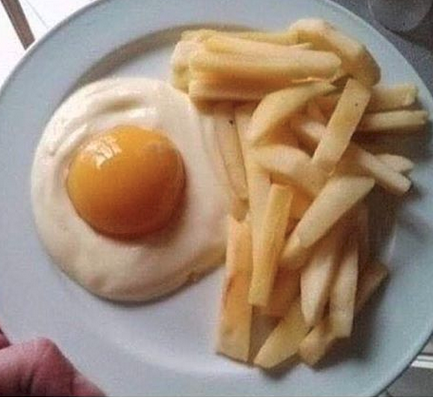
\includegraphics[scale=0.6]{cap01/visao.png}
	\caption{Nova informação}
\end{figure}

Qual será o prato de comida que provavelmente ele associará? Exatamente "Ovo frito e batatas fritas"\footnote{Apesar que se olhar mais de perto verá que isso é iogurte, meio pêssego e tiras de maçã}. No segundo tipo de aprendizado além das imagens dizemos o que cada uma vem a ser, porém ao mostrar a mesma imagem não pense que o computador saberá classificá-la corretamente pois provavelmente se confundirá mais uma vez (assim como você deve ter se confundido).

A resolução com problemas de imagem é bem complicada\footnote{Assim como análise da linguagem, chamada de NLP - \textit{Natural Language Processing}}, pois conseguimos identificar a diferença devido a nossa experiência não apenas visual mas com informações sobre textura, forma e outras que o computador ainda está engatinhando. Por isso o estudo desses algorítimos é algo tão rico e como vimos anteriormente. É muito importante conhecer boa parte dos modelos para decidir qual se ajusta e trabalha melhor aos dados que temos para treiná-los.

\subsection{Algoritmo Não Supervisionado}
Não envolvem um controle direto, aqui o ponto principal do requisito são desconhecidos e ainda precisam ser definidos. Normalmente são usados para: explorar uma estrutura de informação; extrair informações desconhecidas sobre os dados e observar a detecção de padrões.
\begin{description}
	\item[k-means:] é o mais popular, usado para segmentar em categorias exclusivas com base em uma variedade de recursos, por exemplo clientes como seus hábitos de consumo ou casas com seu preço, localidade e área.
	\item[t-Distributed Stochastic Neighbor Embedding:] t-SNE é utilizado para redução de dimensionalidade que é particularmente adequada para a visualização de conjuntos que possuem dados com alta dimensão.
	\item[Principal Component Analysis:] PCA é usado para enfatizar a variação e destacar padrões fortes em um conjunto de dados, de modo a facilitar a exploração e visualização de dados.
	\item[Associate Rule Mining:] ARM para encontrar padrões frequentes, associações, relações e correlação, normalmente usado para fazer análises de cesta de compras. Em termos gerais, é aplicado em várias situações para encontrar associação, padrão frequente nos conjuntos de objetos nos bancos de dados.
\end{description}

\subsection{Algoritmos Supervisionados}
Neste tipo temos dados de valores conhecidos e do ponto de vista da máquina, esse processo é uma rotina de "conectar os pontos" ou achar similaridades entre os dados. Para "alimentar" o algoritmo determinamos que tipo de resultado é desejado ("sim/não", "verdadeiro/falso", a projeção do valor das vendas, a perda líquida de crédito ou o preço da habitação).
\begin{description}
	\item[Regressão linear:] muito utilizado para prever resultados numéricos contínuos, como preços de casas ou ações, umidade ou temperatura de um local, crescimento populacional.
	\item[Regressão logística:] É um classificador popular usado especialmente no setor de crédito para prever inadimplências de empréstimos.
	\item[k-Nearest Neighbors:] k-NN é um algoritmo usado para classificar dados em duas ou mais categorias e é amplamente usado para classificar casas em grupos como caras e acessíveis, com base em preço, área, quartos e toda uma gama de outros recursos.
	\item[Support Vector Machines:] SVM é um classificador popular usado na detecção de imagens e faces, além de aplicativos como reconhecimento de manuscrito.
	\item[Tree-Based Algorithms:] Algoritmos baseados em árvores, como florestas aleatórias ou árvores de decisão ou reforçadas, são usados para resolver problemas de classificação e regressão.
	\item[Naive Bayes:] Este classificador usa o modelo matemático de probabilidade para resolver problemas de classificação.
\end{description}

\subsection{Algoritmos de Aprendizagem por Reforço}
Tratam de situações onde a máquina começa a aprender por tentativa e erro ao atuar sobre um ambiente dinâmico. Desta maneira, não é necessário novos exemplos ou um modelo a respeito da tarefa a ser executada: a única fonte de aprendizado é a própria experiência do agente, cujo objetivo formal é adquirir uma política de ações que maximize seu desempenho geral.
\begin{description}
	\item[Q-Learning:] é um algoritmo de aprendizado baseado em valores. Os algoritmos baseados em valor atualizam uma função com base em uma equação (particularmente neste caso a equação de \textit{Bellman}). Enquanto o outro tipo, baseado em políticas, estima a função de valor com uma política gananciosa obtida a partir do último aprimoramento da política. Q-learning é um aluno fora da política. Significa que aprende o valor da política ideal, independentemente das ações do agente. Por outro lado, um aprendiz de política aprende o valor da política que está sendo executada pelo agente, incluindo as etapas de exploração e encontrará uma política ideal, levando em consideração a exploração inerente à política.
	\item[Temporal Difference:] TD é um agente que aprende em um ambiente por meio de episódios sem conhecimento prévio desse ambiente. Isso significa que a diferença temporal adota uma abordagem de aprendizado sem modelo ou sem supervisão. Podemos considerar isso como uma tentativa e erro.
	\item[Monte-Carlo Tree Search:] MCTS é um método geralmente usado nos jogos para prever o caminho (movimentos) que a política deve seguir para alcançar a solução final vencedora. Jogos como Cubo de Rubik, Sudoku, Xadrez, Go, ou um simples Jogo da Velha têm muitas propriedades em comuns que levam ao aumento exponencial do número de possíveis ações que podem ser executadas. Esses passos aumentam exponencialmente à medida que o jogo avança. Idealmente, podemos prever todos os movimentos possíveis e seus resultados que podem ocorrer no futuro e assim aumentarmos a chance de ganhar.
	\item[Asynchronous Advantage Actor-Critic:] A3C é um dos algoritmos mais recentes a serem desenvolvidos no campo de aprendizado de reforço profundo. Esse algoritmo foi desenvolvido pelo \textit{DeepMind} do Google. Implementa treinamento no qual vários \textit{workers}, em ambiente paralelo, atualizam independentemente uma função de valor global - portanto "assíncrona". Um dos principais benefícios de ter atores assíncronos é a exploração eficaz e eficiente do espaço de estados.
\end{description}

\section{Montagem do Ambiente}\index{Entendimento Geral}
Vemos atualmente uma grande revolução em torno de \textit{Data Science} (falamos em inglês para parecer algo chique) principalmente em torno as ferramentas que tem se atualizado a uma velocidade assustadora. Porém, essas atualizações constantes muitas vezes carregam problemas que podem afetar o seu Sistema Operacional. A pergunta é: Como ficar atualizado e seguro ao mesmo tempo? A única resposta coerente que consegui encontrar foi: Usar a conteinerização para resolver o problema.

Então o ideal é partir atrás de imagens prontas, visitar sites como HubDocker (\url{https://hub.docker.com}) e rezar para encontrar a imagem que nos atenda ou fazer algo melhor e personalizar a imagem.
\begin{figure}[H]
	\centering
\includegraphics[scale=0.2]{cap01/docker.png}
	\caption{Docker e Jupyter para Data Science}
\end{figure}

Essa segunda alternativa é bem mais próxima a realidade de qualquer um que deseje trabalhar de modo efetivo com Ciência de Dados. A personalização de uma imagem no Docker não é um bicho de sete cabeças (no qual a partir do momento que cortamos uma das cabeças nasce mais duas, então sempre imaginei que seriam mais do que sete) mas algo que pode ser facilmente aprendido por qualquer um que "ao menos" saiba usar o terminal de comando do Linux.

\begin{note}[Não sabe nem por onde começar com o Docker?] 
	Não se desespere, baixe um paper sobre o Docker gratuitamente na minha página no Academia.edu (\url{https://iesbpreve.academia.edu/FernandoAnselmo}).
\end{note}

Minha primeira personalização de Imagem\footnote{O objetivo não é termos uma imagem pequena, mas uma PERSONALIZÁVEL, se deseja que seja pequena recomendo que acesse o tutorial disponível em \url{https://jcrist.github.io/conda-docker-tips.html}.} surgiu quando descobri que as versões \textbf{Jupyter} não me atendiam por completo e \textbf{Anaconda} era grande demais. Iremos então trabalhar em uma imagem que possa conter um Jupyter mais adequado e uma Anaconda mas controlada. O resultado foi o seguinte \textbf{Dockerfile} (que obrigatoriamente deve ter esse nome de arquivo):
\begin{lstlisting}
# Base da Imagem
FROM ubuntu:19.10

# Adiciona o metadata para a imagem com o par: chave,valor
LABEL maintainer="Fernando Anselmo <fernando.anselmo74@gmail.com>"
LABEL version="1.2"

# Variaveis de Ambiente
ENV LANG=C.UTF-8 LC_ALL=C.UTF-8 PATH=/opt/conda/bin:$PATH

# Execucoes iniciais:
# Cria a pasta de ligacao
RUN mkdir ~/GitProjects && \
# instala os pacotes necessarios
apt-get update && apt-get install --no-install-recommends --yes python3 && \
apt-get install -y wget ca-certificates git-core pkg-config tree freetds-dev apt-utils && \
# Limpeza basica
apt-get autoclean -y && \
rm -rf /var/lib/apt/lists/* && \
# Configuracao do Jupyter
mkdir ~/.ssh && touch ~/.ssh/known_hosts && \
ssh-keygen -F github.com || ssh-keyscan github.com >> ~/.ssh/known_hosts && \
git clone https://github.com/bobbywlindsey/dotfiles.git && \
mkdir ~/.jupyter && \
mkdir -p ~/.jupyter/custom && \
mkdir -p ~/.jupyter/nbconfig && \
cp /dotfiles/jupyter/jupyter_notebook_config.py ~/.jupyter/ && \
cp /dotfiles/jupyter/custom/custom.js ~/.jupyter/custom/ && \
cp /dotfiles/jupyter/nbconfig/notebook.json ~/.jupyter/nbconfig/ && \
rm -rf /dotfiles && \
# Instalar o Anaconda
echo 'export PATH=/opt/conda/bin:$PATH' > /etc/profile.d/conda.sh && \
wget --quiet https://repo.anaconda.com/archive/Anaconda3-2020.02-Linux-x86_64.sh -O ~/anaconda.sh && \
/bin/bash ~/anaconda.sh -b -p /opt/conda && \
rm ~/anaconda.sh && \
conda uninstall anaconda-navigator && \
conda update conda && \
conda update anaconda && \
conda install nodejs && \
conda update --all && \
# Limpeza basica no Anaconda
find /opt/conda/ -follow -type f -name '*.a' -delete && \
find /opt/conda/ -follow -type f -name '*.pyc' -delete && \
find /opt/conda/ -follow -type f -name '*.js.map' -delete && \
find /opt/conda/lib/python*/site-packages/bokeh/server/static -follow -type f -name '*.js' ! -name '*.min.js' -delete &&  \
# Instalar os temas para o Jupyter
pip install msgpack jupyterthemes && \
jt -t grade3 && \
# Instalar os pacotes
conda install scipy && \
conda install pymssql mkl=2018 && \
pip install SQLAlchemy missingno json_tricks \
gensim elasticsearch psycopg2-binary \
jupyter_contrib_nbextensions mysql-connector-python \
jupyter_nbextensions_configurator pymc3 apyori && \
# Habilitar as extensoes do Jupyter Notebook
jupyter contrib nbextension install --user && \
jupyter nbextensions_configurator enable --user && \
jupyter nbextension enable codefolding/main && \
jupyter nbextension enable collapsible_headings/main && \
# Adicionar a extensao do vim-binding
mkdir -p $(jupyter --data-dir)/nbextensions && \
git clone https://github.com/lambdalisue/jupyter-vim-binding $(jupyter --data-dir)/nbextensions/vim_binding && \
cd $(jupyter --data-dir)/nbextensions \
chmod -R go-w vim_binding && \
# Remover o que nao eh necessario
conda clean -afy && \
apt-get remove -y wget git-core pkg-config && \
apt-get autoremove -y && apt-get autoclean -y && \
# Adicionar o Git ao Jupyter Lab
pip install --upgrade jupyterlab-git && \
jupyter lab build

# Configurar o acesso ao Jupyter
WORKDIR /root/GitProjects
EXPOSE 8888
CMD jupyter lab --no-browser --ip=0.0.0.0 --allow-root --NotebookApp.token='data-science'
\end{lstlisting}

Tento manter sempre o script o mais documentado possível deste modo posso remover ou adicionar propriedades sem me incomodar muito. Para criarmos a imagem é muito simples, supondo que a localização do script esteja em uma pasta chamada docker-data-science, então na pasta anterior digitar o comando: \\
{\ttfamily\$ docker build -t fernandoanselmo/docker-data-science docker-data-science}

Obviamente que "fernandoanselmo/docker-data-science" pode ser alterado para o nome que desejar, porém na essência isso cria uma imagem que contém além do sistema operacional uma versão completa do Jupyter (com a inclusão de várias funcionalidades) para a realização do nosso trabalho como Cientista de Dados. 

Mas isso é muito complicado e não entendo nada disso! Sem problemas, basta saltar toda essa parte de criação e construção da imagem para o próximo tópico seguindo comando a comando, pois este foi publicado do \textbf{DockerHub} e será baixado sem problemas.

Agora o comando: \\
{\ttfamily\$ docker run -d -t -i -v ---privileged /dev/ttyACM0:/dev/ttyACM0 -v \\ $\sim$/Aplicativos/ipynb:/root/GitProjects ---network=host \\
	 ---name meu-jupyter fernandoanselmo/docker-data-science}
 
Realiza a criação de um contêiner. Vamos aos detalhes, após a opção -v aparece a expressão "$\sim$/Aplicativos/ipynb", essa se refere a uma determinada pasta no sistema operacional onde serão armazenados os Notebooks produzidos. Abrir o navegador no endereço \url{http://localhost:8888} e obtemos o seguinte resultado:
\begin{figure}[H]
	\centering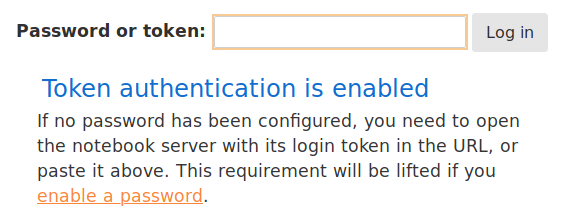
\includegraphics[scale=0.5]{cap01/paginaSenha.png}
	\caption{Jupyter solicitando o Token}
\end{figure}

A senha do token está definida na última linha do Script como "data-science", após informá-la o jupyter está pronto para trabalharmos:
\begin{figure}[H]
	\centering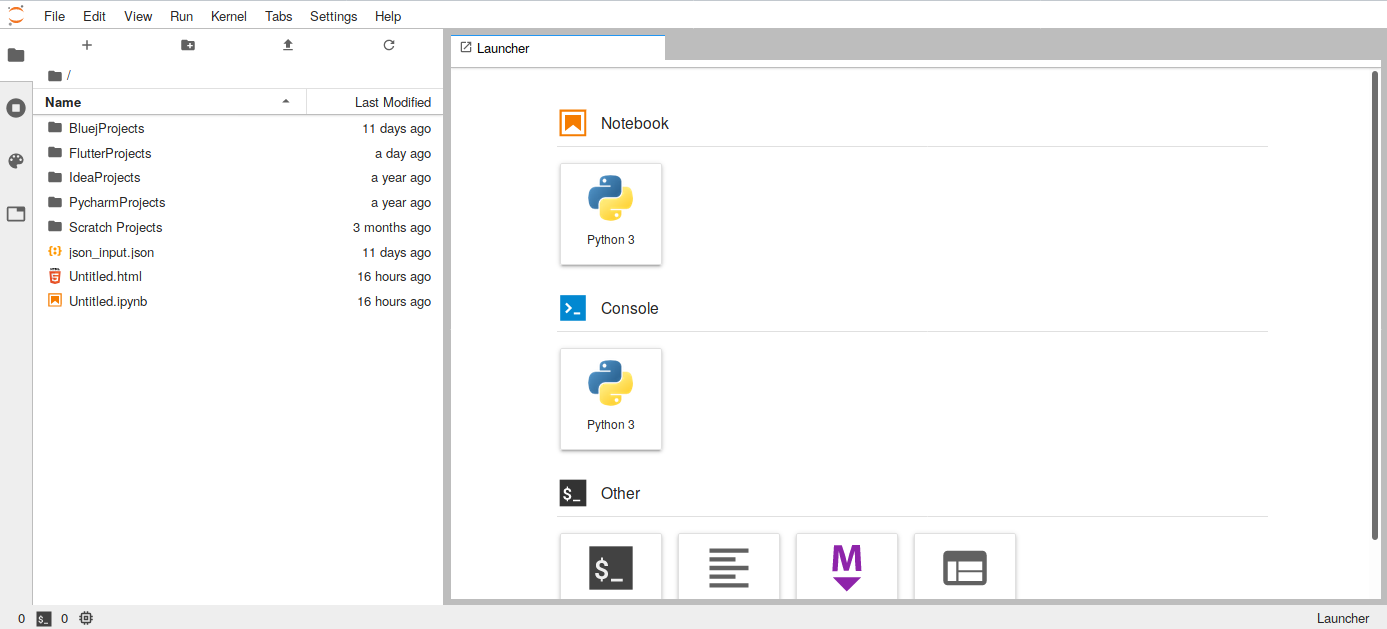
\includegraphics[scale=0.3]{cap01/jupyterLab.png}
	\caption{Jupyter Lab pronto}
\end{figure}

A maior vantagem que agora possuímos um ambiente com o \textbf{Jupyter Lab} completamente controlado incluindo temas e sincronização com o \textbf{Github}. Os próximos comandos são bem mais simples, tais como: \\
{\ttfamily\$ docker stop meu-jupyter} \\
{\ttfamily\$ docker start meu-jupyter}

Respectivamente para encerrar e iniciar o contêiner. Oh não! Agora estou preso, não posso mais fazer atualizações. Devemos entender que os contêineres são \textbf{dinâmicos}. Precisamos instalar o Keras/TensorFlow, acessar o contêiner (com ele já iniciado): \\
{\ttfamily\$ docker exec -it meu-jupyter /bin/bash}

E instalamos normalmente, como se estivesse em uma máquina com o Ubuntu (com os poderes de superusuário): \\
{\ttfamily\# conda install -c conda-forge keras}

Pronto uma vez testado podemos optar por manter só nesse contêiner, ou então modificar o Script para ao criarmos novos contêineres e estes serão criados com essa funcionalidade embutida.

Verificar qual a versão do Python que está a nossa disposição, em uma célula do Notebook digite:
\begin{lstlisting}
!python --version
\end{lstlisting}

Ao pressionarmos Ctrl+Enter será mostrada a versão 3.7.7. Agora podemos testar e executar qualquer ferramental sem nos preocuparmos em corromper a máquina. Talvez, no máximo, perdermos um contêiner.
	
\clearpage
% Conceitos Introdutórios
%------------------------------------------------------------------------------------
%	CHAPTER 2
%------------------------------------------------------------------------------------
\chapterimage{headerCap.png}
\chapter{Falando com Ubuntu}

\begin{remark}
O computador não é mais apenas um dispositivo, é uma extensão da sua mente e uma porta de outra para a mente dos outros. (Mark Shuttleworth) 
\end{remark}

\section{Coisas Ubuntu}\index{Falando com Ubuntu}
Acho muito engraçado como existe um caso de paixão ou puro ódio em relação a Ubuntu. Não sei se é inveja por ser a distribuição mais utilizada, ou chateação pois é muito fácil de usar, ou simples paranoia mesmo. Alguns defensores radicais do software livre pregam que Ubuntu não é 100\% Software Aberto, pergunto, e daí? Vamos imaginar que a \textbf{NVidia} produziu um drive para sua placa e a empresa simplesmente resolveu não divulgar os fontes, qual o problema disso? Quero saber é: A placa que paguei bons quantos dólares (porque não foi em reais) vai funcionar com aquele super jogo, ou devo (como bom usuário do Software Livre) exigir que no meu computador só entre software aonde posso ver os fontes senão estarei ``defraudando'' alguma organização.

Outra alegação em ser tudo aberto é porque senão a \textbf{Canonical} pode enviar informações do meu computador sobre o que estou fazendo. Falando sério, acredita realmente que Google, Microsoft, Oracle, Canonical ou qualquer outra empresa está interessada no que está fazendo? Essas empresas estão interessados é no que o coletivo está fazendo, pois precisam desses dados como forma de prospectar novos negócios, é uma simples pesquisa no qual somos todos participantes ativos. Não gosta disso? Então recomendo que desligue sua Internet, tire a bateria de seu telefone, puxe o cabo da tomada da televisão, tire as pilhas do rádio, quebre seu cartão de crédito e não esqueça de levar um colchão (de palha) para a caverna que pretende morar a partir de hoje.

Caso contrário, siga os seguintes passos: \vspace{-1em}
\begin{enumerate}[noitemsep]
 \item Abrir o aplicativo \textbf{Programas e atualizações}
 \item Na aba \textbf{Drives Adicionais}, ativar (caso exista) os drivers proprietários (NVIDIA, ATI, Broadcom)
 \item Na aba \textbf{Outros Programas}, ativar o repositório ``Parceiros da Canonical'' para ter acesso a alguns aplicativos extras.
\end{enumerate}

Quando, ainda na versão da interface gráfica Unity, surgiu a barra lateral e muita gente não gostou. Só que esta barra contém os aplicativos que estão abertos e ao posicionar o mouse sobre eles e usar o scroll (a rodinha do meio) é trazido para a tela da frente, ou seja, tornou muito mais fácil e rápido acessar qualquer aplicativo. A barra foi tão importante que no retorno do Gnome decidiram criar uma versão desta.

Outro xingamento em relação a interface gráfica Unity foi que muitos usuários de Linux nasceram acostumados com o KDE ou o Gnome, e esse último era o padrão do Ubuntu até ser substituído pela Unity. Como nasci para este mundo na 14.04 não sei se o Gnome era melhor (pois quando usava achava sempre mais bonito o KDE do Kurumin), só que o Unity além de muito fácil em configurar, junto com o Compiz permitia que personalizasse a área de trabalho do jeito que gosto. Com a volta do Gnome simplesmente me adaptei sem me importar muito.

Acho que o real problema das pessoas é que não gostam de \textbf{mudanças}. Estamos ali naquela tranquilidade em um ambiente que conhecemos e de repente, acontece. Alguém vem com uma ideia doida e tudo muda, acho que mudança faz parte do mundo. Desde que me conheço por gente, se não me adaptasse hoje estaria programando em um terminal com PL1 ou Algol. Uma das características principais do ser humano e adaptação, porém primeiro existe a reclamação. 

Não sou e nem pretendo ser vítima disso que as pessoas pregam sobre Ubuntu, escolhi porque achei a distribuição mais fácil e mais agradável de lidar e até o momento não me arrependo da decisão e no dia que mudar será porque descobri algo melhor e mais fácil de utilizar.

\subsection{Curiosidade das Versões}\index{Conceitos Introdutórios}
Por ano são lançadas 2 versões do Ubuntu, por exemplo em 2014 foram lançadas as versões 14.04 e 14.10. O primeiro número corresponde ao ano da versão e o número adjacente ao seu mês de lançamento. Então, 14.04 foi lançada no mês de abril enquanto que a 14.10 lançada no mês de outubro no ano de 2014. Outro detalhe é que a primeira normalmente traz mudanças mais profundas enquanto que a segunda fica a cargo de um pacote completo de correções (como aqueles famosos \textit{Service Packs} lançados pela Microsoft) ou seja, se quiser muita estabilidade opte sempre pela segunda ou versões LTS.

Uma versão LTS significa que possui um longo tempo de suporte (\textit{Long Term Support}) e atualmente significa que a versão terá suporte oficial da Canonical por 5 anos. As outras são subtituladas Regulares (\textit{Regular}) que são como laboratórios de testes para as versões LTS, seu suporte é de 2 anos e utilizam os pacotes mais recentes.

Eis uma lista com todas as versões lançadas até este livro:
\begin{center}
 \begin{longtable}[h!]{l|l|l}
  \textbf{Versão} & \textbf{Code Name – Animal} & \textbf{Kernel} \\
  \hline
  4.10 & Warty Warthog (O porco-africano verruguento) & 2.6.8 \\
  5.04 & Hoary Hedgehog (O ouriço grisalho) & 2.6.10 \\
  5.10 & Breezy Badger (O texugo fresco) & 2.6.12 \\
  6.06 LTS & Dapper Drake (O pato doméstico estiloso) & 2.6.15 \\
  6.10 & Edgy Eft (A salamandra hi-tec) & 2.6.17 \\
  7.04 & Faisty Fawn (O cervo jovem bravo) & 2.6.20 \\
  7.10 & Gutsy Gibbon (O gibão1 corajoso) & 2.6.22 \\
  8.04 LTS & Hardy Heron (A garça durona) & 2.6.24 \\
  8.10 & Intrepid Ibex (O bode intrépido) & 2.6.27 \\
  9.04 & Jaunty Jackalope2 (A coelho antílope elegante) & 2.6.28 \\
  9.10 & Karmic Koala (O koala kármico) & 2.6.31 \\
  10.04 LTS & Lucid Lynx (O lince lúcido) & 2.6.32 \\
  10.10 & Maverick Meerkat (O suricate vagabundo) & 2.6.35 \\
  11.04 & Natty Narwhal (O narval inteligente) & 2.6.38 \\
  11.10 & Oneiric Ocelot (A jaguatirica onírica) & 3.0 \\
  12.04 LTS & Precise Pangolin (O pangolim preciso) & 3.2 \\
  12.10 & Quantal Quetzal (o quetzal quântico) & 3.5 \\
  13.04 & Raring Ringtail (O bassarisco ávido) & 3.8 \\
  13.10 & Saucy Salamander (A salamandra atrevida) & 3.11 \\
  14.04 LTS & Trusty Tair (A cabra selvagem fiel) & 3.13 \\
  14.10 & Utopic Unicorn (O unicornio utópico) & 3.16 \\
  15.04 & Vivid Vervet (O macaco vívido) & 3.19 \\
  15.10 & Wily Werewolf (O lobisomem astuto) & 4.1 \\
  16.04 LTS & Xenial Xerus (O xerus hospitalário) & 4.4 \\
  16.10 & Yakkety Yak (O iaque falador) & 4.8 \\
  17.04 & Zetty Zapus (O zapus enérgico) & 4.10 \\
  17.10 & Artful Aardvark (O porco-formigueiro astuto) & 4.13 \\
  18.04 LTS & Bionic Beaver (O castor biônico) & 4.15 \\
  18.10 & Cosmic Cuttlefish (O choco côsmico) & 4.18 \\
  19.04 & Disco Dingo (O dingo dançante) & 5.0 \\
  19.10 & Eoan Ermine (O eoan arminho) & 5.3 \\
  20.04 LTS & Focal Fossa (A fossa focal) & 5.4
 \end{longtable}
\end{center}\vspace{-3em}

Os ``apelidos'' dados para cada versão é a formação das palavras \textbf{adjetivo + animal}. E esse adjetivo não é uma palavra qualquer, possui a mesma letra inicial do animal em questão, e que a partir da versão 6.06 possui uma sequencia alfabética.
\\[3mm]
\begin{dica}[Não precisa instalar o Ubuntu para usá-lo]
	Nem ao menos colocar um DVD (ou CD) Live, basta acessar o seguinte endereço \url{http://www.ubuntu.com/tour/en/} para entrar em um simulador. Experimente pois é totalmente indolor. \url{http://old-releases.ubuntu.com/releases/} este site é para todo tipo de saudosista que deseja encontrar uma versão antiga do Ubuntu.
\end{dica}

\subsection{Como atualizar a versão do sistema?}\index{Conceitos Introdutórios}
Se já possui o Ubuntu instalado a atualização é realizada através da confirmação do desejo de instalar uma nova versão. Para que a janela de escolha possa ser mostrada, abra o aplicativo “Programas e Atualizações” e na aba “Atualizações”, verifique se a opção “Notificar-me de uma nova versão do Ubuntu” está selecionada com a escolha a qualquer nova versão.
\begin{figure}[H]
 \centering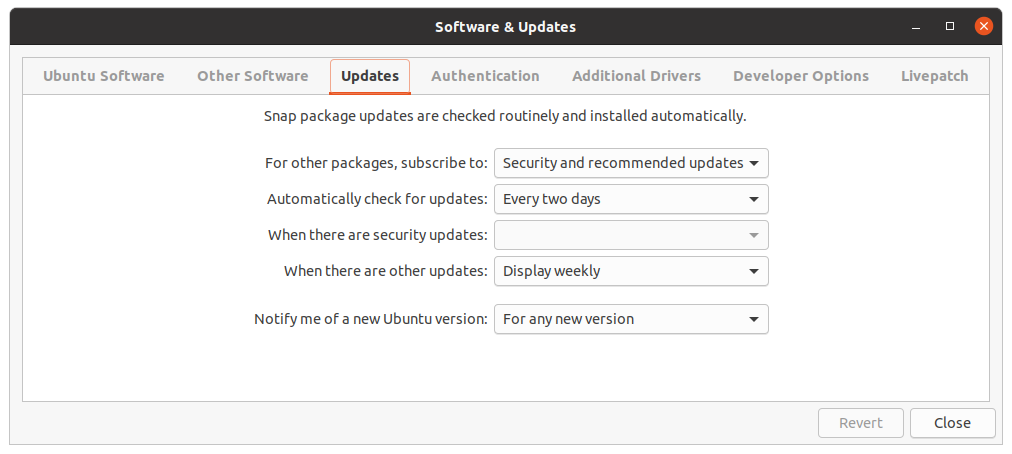
\includegraphics[scale=0.4]{cap02/atualizar.png}
 \caption{Verificar esta opção}
 \end{figure}

Se desejar que a atualização seja realizada agora, entrar no terminal e usar os seguintes comandos: \\
{\ttfamily\$ sudo apt update \&\& sudo apt dist-upgrade \\
\$ sudo do-release-upgrade}

\section{Termos usados pelos usuários}\index{Falando com Ubuntu}
Caso venha a participar de listas de discussão ou de conversas sobre o Linux é bem provável que ouça uns termos que não ouviria em discussões sobre o Windows. E esses termos não se restringe apenas a Kernel ou Distros, vai muito além disso, vejamos os mais comuns:
\begin{itemize} \vspace{-1em}
   \item \textbf{Boot Loader} – refere-se ao programa de inicialização, é aquele programa que define qual sistema operacional será chamado. Por exemplo: GRUB ou ISOLINUX.
   \item \textbf{Serviços ou Processos} – são os aplicativos que estão rodando em background no computador neste exato momento.
   \item \textbf{File System} – a forma como são organizados e armazenados seus arquivos no sistema operacional, isso é definido durante o processo de formatação. Por exemplo: ext3, ext4, FAT, XFS e NTFS.
   \item \textbf{X Window} – refere-se a toda interface gráfica, formada por: Ambiente Desktop, Gerenciador de Janelas e X11 (sistema X Window).
   \item \textbf{Ambiente Desktop} – refere-se ao ambiente gráfico que visualizamos que pode ser, GNOME, KDE, Xfce, Fluxbox e Unity.
   \item \textbf{Linha de Comando} – é a interface para digitar os comandos (a janela de terminal).
   \item \textbf{Shell} – é o interpretador de comandos, sua função é de interpretar o comando dado no terminal e diz ao sistema operacional o que fazer.
\end{itemize}
Existem também alguns comandos que todo administrador do sistema conhece e muitas vezes são utilizados nas lista de discussão para a resolução de um determinado problema.

Mostrar todas as mensagens do Kernel, é útil para resolução de problemas de inicialização do sistema ou algum erro que pode estar acontecendo recorrentemente: \\
{\ttfamily\$ dmesg}

Observar detalhes da CPU: \\
{\ttfamily\$ cat /proc/cpuinfo}

Observar detalhes da memória: \\
{\ttfamily\$ cat /proc/meminfo}

Verificar quando ocorreram as últimas inicializações ocorridas no sistema: \\
{\ttfamily\$ last reboot}

Descobrir se existe alguém ``pendurado'' no nosso computador: \\
{\ttfamily\$ w}

\section{Reiniciar o ambiente gráfico}\index{Falando com Ubuntu}
Fiquei pensando que meu problema com o Windows poderia ter sido resolvido com algo bem simples – Reiniciar as propriedades gráficas. Por exemplo, acabamos de instalar um drive para uma placa gráfica e arrebentamos completamente com a interface gráfica. E o que desejo propor é muito simples: Sem nenhum ponto de restauração desejo aplicar um RESET nas propriedades gráficas e voltá-las ao padrão do qual estavam quando instalei o sistema. Tenho diversos aplicativos instalados, não quero perdê-los e não tenho nenhum ponto de restauração.

E esse é o grande problema do Windows, muitas coisas são tão voltadas ao iniciante que o sistema esquece que existem usuários mais avançados para corrompê-lo. Outra problema é ser administrador de um curso de informática, são vários computadores e ao finalizar uma turma cada computador apresenta uma cara diferente (além de outras coisas). Existem soluções Windows para isso? Claro que sim, vamos a algumas: \vspace{-1em}
\begin{itemize}[noitemsep]
 \item Criar um ponto de restauração antes da aula, e usá-lo depois. Problema: Perderemos qualquer coisa que o professor tenha instalado. 
 \item Criar uma imagem do sistema e restaurá-lo em seguida. Problema: O mesmo anterior. 
 \item Não permitir que o aluno altere qualquer coisa no sistema operacional. Problema: E como o aluno vai instalar os aplicativos que o professor deseja? Vai ter que acabar permitindo que sejam instalados pelo aluno.
 \item Ter máquinas com tudo previamente instalado. Problema: Adeus aula prática de instalação e o aluno que se vire em casa para instalar tudo.
\end{itemize}

Ou seja, em qualquer dessas soluções acabamos esbarrando em problemas. Isso porque nem citei a solução de aplicativos que fazem esse controle e que envolvem custos. Quero permitir (assim como ter) liberdade de poder mudar o sistema da forma como quiser e depois, se algo der errado, magicamente, dar um comando RESET e tudo voltar a normalidade. Para reiniciar o ambiente gráfico GNome necessitamos realizar os seguintes passos no terminal.

Acessar o diretório: \\
{\ttfamily\$ cd /etc/init.d}

Para reiniciar a interface gráfica: \\
{\ttfamily\$ sudo service gdm restart}

Para interromper a interface gráfica: \\
{\ttfamily\$ sudo service gdm stop}

Para iniciar a interface gráfica: \\
{\ttfamily\$ sudo service gdm start}
\\[3mm]
\begin{dica}[Não se desespere] Utilize esses comandos quando a coisa estiver realmente feia, lembre-se que é sempre ideal ter uma cópia de segurança de todos seus arquivos particulares. 

Outra dica, muitas das configurações particulares dos aplicativos ficam na pasta: $\sim$/.config então, em muitos dos casos basta eliminar a configuração particular de um determinado aplicativo em questão que possa estar apresentando problemas.
\end{dica}

Sua interface está lenta ou estranha? Não é necessário sair da sessão ou reiniciar tudo, basta pressionar \textbf{ALT + F2} e digitar o comando ``r''.

\section{Existe vida além do Ubuntu}\index{Falando com Ubuntu}
Ubuntu não é a única distribuição filha da Debian e derivam várias outras distribuições, entre as mais conhecidas estão: \vspace{-1em}
\begin{itemize}
 \item \textbf{Ubuntu Studio} – Provavelmente se não usasse Ubuntu seria esta distro que usaria, vem com muitos aplicativos instalados para transformar o computador em uma central de edição de Música, Imagem e Vídeo.
 \item \textbf{Xubuntu} – Com base em Xfce que, segundo seus criadores, busca ser um sistema elegante e muito fácil de usar.
 \item \textbf{Kubuntu} – Com base em KDE. É uma alternativa ao uso do Gnome e Unity fortemente presentes e por muito pouco não foi minha distribuição escolhida pois gostava muito do visual da distribuição Mandriva (da Conectiva).
 \item \textbf{Edubuntu} – Totalmente focada para ser a distribuição ideal para escolas e estudantes em geral.
 \item \textbf{Linux Mint} – É a grande concorrente, e busca a facilidade de uso através de um ambiente gráfico visualmente explorado.
 \item \textbf{Knoppix} – é uma Live CD também baseado em KDE.
 \item \textbf{Kanotix} – é a que mais se parece com a Avó (Debian) sendo também uma Live CD.
 \item \textbf{Damm Small Linux} – Este é a pequenininha da família (possui apenas 50 Mb) é outra Live CD baseado na Knoppix.
\end{itemize}

As quatro primeiras distros são basicamente uma cópia da Ubuntu destinadas as suas particularidades. No Brasil, o Governo Federal lançou a \textbf{Linux Educacional}\footnote{Em \url{https://linuxeducacional.c3sl.ufpr.br/}} também com base na Ubuntu (pode-se dizer que é uma Edubuntu Brasileiro) que nasceu no Centro de Experimentação em Tecnologia Educacional (CETE) do Ministério da Educação (MEC) e atualmente (na versão 6.1) está a cargo da Universidade Federal do Paraná. E foi exatamente esta distribuição que me fez voltar a utilizar o Linux.

\section{Janela do Terminal}\index{Falando com Ubuntu}
A primeira vez que tentei utilizar Linux na vida foi quando comprei um livro, ``Servidor Internet com Linux'' de Kevin Reichard, vinha com um CD com o \textbf{Slackware OS - Versão 2.2}. Quando um colega que entendia muito do Linux conseguiu instalar no meu computador juro que me senti como se tivesse adquirido um daqueles extremamente antigos, cadê a janela gráfica que o Windows 3.11 possuía e que facilitava muito meu trabalho? Como iria instalar meus aplicativos? O que iria fazer com um sistema operacional que tinha uma tela estranha para mim, não tinha a menor noção dos comandos e a linguagem C como pano de fundo\footnote{Para entender meu drama, era um programador oriundo do Pascal}.
\begin{figure}[H]
 \centering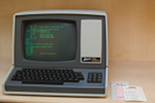
\includegraphics[scale=4.5]{cap02/computadorAntigo.png}
 \caption{Computador antigo da minha época}
\end{figure}

Minha segunda tentativa foi durante o planejamento do meu livro de PHP, tinha uma pilha de CDs de distros, tinha adquirido naquelas revista que se encontrava aos quilos nas bancas (outra metade dos meus CDs eram Demos de jogos – Sim, houve época que nos divertíamos com uma ou duas fases de um jogo e isso durava horas). Como o PHP, Apache e MySQL eram totalmente livres nada mais justo seria que também usasse um sistema livre para o livro, só que queria que a instalação fosse fácil para meu leitor (afinal não estaria ao seu lado para instalar o ambiente). Funcionava assim, pegava um CD, instalava a distro, tentava colocar o Apache e um editor de modo simples (em muitas o MySQL já vinha instalado por padrão), não dava muito certo (ou era muito complicado) e então mudava de distro (e de CD) o que significava ter que formatar novamente o computador. Resultado que meus dois livros de PHP são escritos para o Windows.

Vou ser bem franco, achava o Linux um Sistema Operacional para os outros. Ainda tentei usar sem muito sucesso me adaptar a Kurumin (uma LiveCD brasileiro) e a Mandriva, mas em momento nenhum via isso como substituto ao Windows, eram apenas para pessoas que adoravam perder muito tempo em fazer algo que resolvia com alguns cliques.

Durante muito tempo achei que nunca usaria esse sistema, até um dia que meu filho meu deu seu Netbook e, não sei porque, resolvi instalar o \textbf{Linux Educacional}, finalmente vi que tinham domesticado o Pinguim e que poderia ser usado para alguma coisa boa. Usei esse computador na faculdade e em nenhum momento me arrependi.

Minha mudança definitiva aconteceu com todos os problemas que citei no começo deste livro, resolvi usar o Linux mais uma vez e de vez. Uma as recomendações que recebi foi: ``Instale o sistema sem a parte gráfica que aprenderá muito mais'', devo confessar que foi a coisa mais IDIOTA que ouvi nos meus 25 anos de informática. Isso soou como alguém dizendo: ``Jogue fora seu computador e use novamente seu TK-83C ou que tal trocar o LibreOffice pelo WordStar ou RedatorPC''.

Quero meu computador para editorar esse livro, fazer meu trabalho da faculdade, programar com um belo editor colorido, baixar a interface do Arduíno, usar aplicativos que comumente uso no meu trabalho, assistir um vídeo, ouvir uma boa música e por aí vai e isso não tem nada a ver com \textbf{ps aux | grep [nome]} e boa sorte para quem sabe o que isso faz.
\\[3mm]
\begin{dica}[Consoles do Linux] Quer ter a experiência de ficar puramente em modo terminal? Então pressione as teclas \textbf{Ctrl + Alt + F2} (existem 6 consoles do F1 a F6). Para retornar ao modo gráfico pressione as teclas \textbf{Ctrl + Alt + F1}.
\end{dica}

No que puder evitar de usar o terminal, evitarei. Não espere encontrar aqui referência aos comandos \textbf{tail} ou \textbf{cd}, o que é a pasta \textbf{/etc} ou \textbf{/opt} ou qualquer coisas dessas. Tentarei e irei simplificar tudo ao máximo, algumas vezes teremos que botar um pouco a mão no terminal mas nada que consiga assustá-lo muito e talvez consigamos aprender a usá-lo sem muitos problemas. Garanto que atualmente a coisa mais interessante a se fazer em uma janela do terminal é digitar o seguinte comando: \\
{\ttfamily\$ apt moo}

Para aqueles que não gostam de fazer as coisas no modo gráfico recomendo que parem imediatamente de ler este livro e procure pelo \textbf{Guia FOCA} que está disponível livremente na Internet. Aqui tentarei deixar as coisas mais fáceis possíveis e isso significa: \vspace{-1em}
\begin{enumerate}[noitemsep]
 \item Mostrar sempre a facilidade gráfica da Distribuição Ubuntu
 \item Dizer que sim, usar Ubuntu é tão fácil quanto usar Windows
 \item Dizer que sim, minha avó (se estivesse viva) podia usar Ubuntu sem problemas
 \item Dizer que sim, acredito que minha avó usa Ubuntu no ``Nosso Lar''.
\end{enumerate}
E pense bem meu amigo que adora o terminal pois passou um bom tempo nessa tela para aprender a usar o sistema: ``Meus Parabéns'' pois será absolutamente necessário e terá emprego garantido (ou quem sabe ganhar muito dinheiro prestando consultoria) quando 90\% do mundo usar uma Distro com base no Linux, só que essa faixa de pessoas ainda utilizam o Windows. Desse modo, vamos parar de besteira e começar a ensinar ao usuário novato que as distros de Linux mudaram e estão amigáveis, mais gráficas e fáceis de usar. Quem sabe assim consigamos difundir a ideia de um sistema operacional totalmente livre.

Devemos brigar pelo que é importante, nos educadores precisamos (alias, temos a obrigação de) lançar cursos para mostrar que o Linux pode ser usado por um usuário iniciante. Parar de tentar empurrar comandos de tela preta goela abaixo no qual o aluno aprenderá de qualquer modo ao longo do percurso, em ``doses homeopáticas'' e não através de uma injeção de Bezetacil.

\section{Aplicativos Comuns, Áreas, PA e Dash}\index{Falando com Ubuntu}
O que aprendi foi que toda mudança nunca é muito simples, usamos diversos aplicativos junto com o sistema operacional para realizarmos nossas tarefas diárias (alguns aplicativos até existem para ambos os ambientes).

Abaixo temos uma relação dos aplicativos mais comumente utilizados entre os sistemas Windows e Linux, e por favor não interprete isto como ``obrigatoriamente deve-se utilizar este'', como disse é apenas um paralelo entre os aplicativos dos sistemas:
\begin{center}
 \begin{longtable}[h!]{l|l|l}
  \textbf{Função} & \textbf{Windows} & \textbf{Linux} \\
  \hline
  Suíte de Escritório & MS-Office & LibreOffice \\
  Editor Leve de Documentos & Notepad & gEdit \\
  Editor com Expr. Regular & Notepad++ & Geany \\
  Diagramador de Publicação & Pagemaker ou inDesign & Scribus \\
  Aplicativo de Email & Outlook & Thunderbird \\
  Navegador Web & Edge & Mozilla Firefox \\
  Leitor de PDF & Adobe Reader & Evince \\
  Tocador Multimídia & Windows Media Player & Totem \\
  Tocador de Música & Winamp & Audacity \\
  Gravador de CD/DVD & Nero Burning ROM & Brasero \\
  Gerenciador de Fotos & Picasa & Shotwell \\
  Editor Gráfico & Adobe Photoshop & Gimp \\
  Mensagem Instantânea & Windows Live Messenger & Empathy \\
  Aplicação VoIP & Skype & Ekiga \\
  Cliente de BitTorrent & uTorrent & Transmission \\
  Cliente de ed2K & eMule & Amule \\
  Firewall & Próprio do Windows & Gufw
 \end{longtable}
\end{center} \vspace{-3em}

Essa relação é somente um comparativo entre os aplicativos mais frequentes usados em seus ambientes, por exemplo usava o \textbf{Gimp} e o \textbf{Scribus} no Windows para criar a ReviSE\footnote{Em \url{http://fernandoanselmo.orgfree.com/wordpress/?page_id=173}} sem qualquer problema, mas neste ambiente é muito mais comum os usuários se utilizarem do \textbf{Photoshop} e o \textbf{Pagemaker}.

Facilmente percebe-se que não coloquei na relação qualquer ambiente de desenvolvimento (Eclipse - Netbeans - Sublime) ou bancos de dados. Essa é somente a relação de aplicativos comumente utilizados, são instalados a partir do modo gráfico e possuem similaridades de funções.

Um fator curioso a se observar aqui é que no ambiente Windows os aplicativos são todos pagos ou gratuitos, enquanto que no Linux a grande maioria é Livre ou Open Source. Como se pelo simples fato de estar utilizando um sistema nesta categoria fossemos atraídos para esse mundo.

\subsection{Áreas de Trabalho}\index{Falando com Ubuntu}
Um dos maiores diferenciais entre os sistemas são as Áreas de trabalho. Para quem está habituado ao Windows, esta funcionalidade não faz muito sentido. No entanto, quem começa a usar as áreas de trabalho depois não quer outra coisa, pois realmente aumentam drasticamente a produtividade. Pressione o símbolo do Windows (chamado Super) no teclado (entre as teclas \textbf{Ctrl} e \textbf{Alt}) e na lateral direita é onde estão posicionadas.

Sua função é a de criar ambientes separados para diferentes conjuntos de aplicativos. Isso permite uma melhor organização dos aplicativos abertos por temas ou a de utilizar como áreas de descarga para aplicativos que não estão sendo usados no momento, e isso reduz drasticamente o congestionamento na barra de tarefas. \vspace{-1em}
\begin{itemize}
 \item Para navegar por entre as áreas de trabalho use a combinação das seguintes teclas:\textbf{Ctrl + Alt + $\uparrow$} ou \textbf{Ctrl + Alt + $\downarrow$}
 \item Três maneiras de levar um aplicativo aberto para outra área de trabalho:
 \begin{enumerate}
  \item Pressionar \textbf{Ctrl + Shift + Alt + [Direcional]}
  \item Pressionar \textbf{[super]} e arraste-o para outra área
  \item Pressionar \textbf{Alt + [barra espaço]} e no menu que aparece selecionar a opção Mover para qual Área de trabalho desejada
 \end{enumerate}
\end{itemize}

\subsection{PA – Programas e atualizações}\index{Falando com Ubuntu}
Para começarmos a falar sobre aplicativos vamos entender um pouco do PA, não se assuste com o nome pois esse é o gerente responsável por descobrir e conhecer todos os repositórios, manutenções do sistema, o que deve ou não ser instalado. \\[3mm]
Está dividido em 7 abas: Aplicativos Ubuntu, Outros programas, Atualizações, Autenticação, Drivers adicionais, Opções para Desenvolvedores e LivePatch.
\begin{figure}[H]
 \centering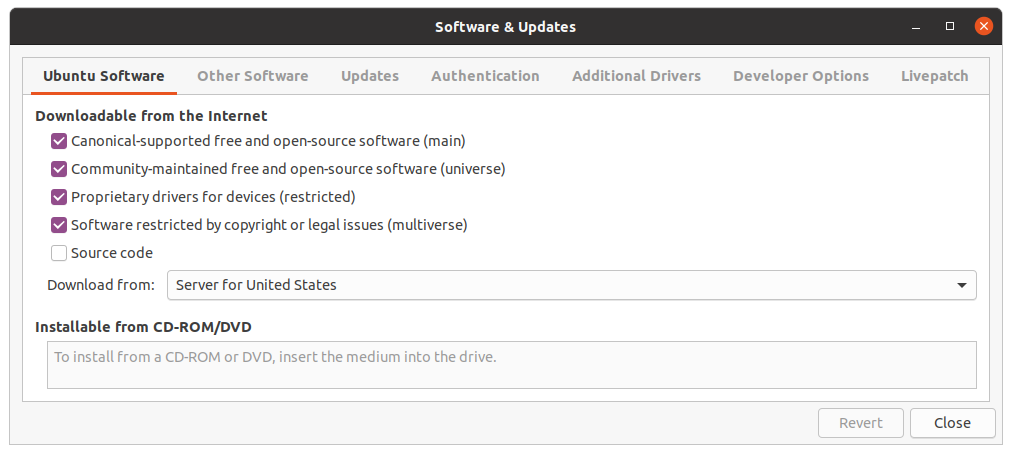
\includegraphics[scale=0.4]{cap02/progsAtualizacoes.png}
 \caption{Programas e Atualizações}
\end{figure}

Nesta primeira aba, mostrada na figura, define quais serão os aplicativos que estarão disponíveis na Loja. As opções são: \vspace{-1em}
\begin{itemize}[noitemsep]
 \item Main – possuem o suporte oficial da Canonical e dificilmente darão qualquer problema com o sistema operacional.
 \item Universe – mantidos pela comunidade, porém, não são oficiais dos desenvolvedores Ubuntu. 
 \item Restricted – proprietários e em sua maioria drivers necessários. 
 \item Multiverse – proprietários e de código fechado. 
\end{itemize}

A última aba se refere ao serviço da Canonical chamado de Livepatch. Tem a função de aplicar correções críticas no sistema sem a necessidade de reiniciar. Essas podem envolver segurança ou partes da infraestrutura de suporte a pacotes. Porém para acessar esse serviço é necessário primeiro criar uma conta (gratuita) na \textbf{Ubuntu One}.

\subsection{Dash}\index{Falando com Ubuntu}
Antes de começarmos a explorar alguns desses aplicativos (e outros) vamos falar da área na qual estão localizados que é conhecida como Dash - Para acessá-la clique no quadrado de pontinhos que fica no inferior da barra lateral:
\begin{figure}[H]
 \centering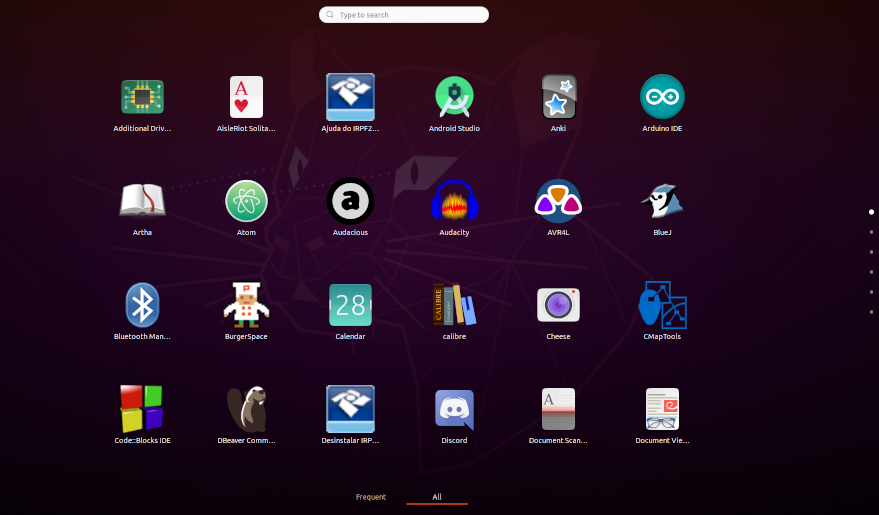
\includegraphics[scale=0.4]{cap02/dash.png}
 \caption{Dash}
\end{figure}

Poderia dizer que é a janela mais importante do sistema pois através desta é possível acessar todos os aplicativos disponíveis no sistema. Para acessar um determinado aplicativo basta digitar seu nome.
\\[3mm]
\begin{dica}[Usando aplicativos] A partir de agora toda vez que citar o aplicativo, bastará ir nessa janela e digitar seu nome, não farei mais referência a isso.
\end{dica}

Não tenha a menor vergonha de pedir ajuda, faço isso constantemente nesse sistema, abra o Dash e digite a palavra \textbf{ajuda} e a seguinte tela será mostrada:
\begin{figure}[H]
 \centering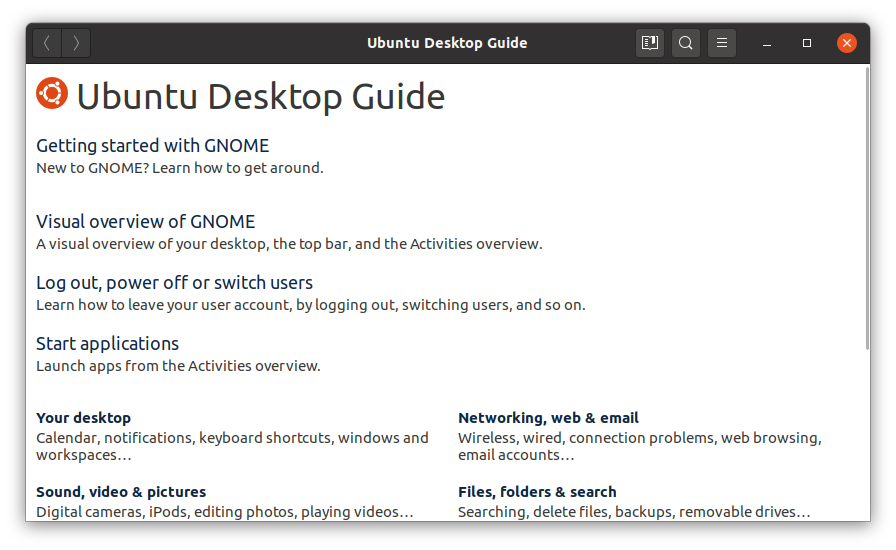
\includegraphics[scale=0.4]{cap02/ajuda.png}
 \caption{Janela de Ajuda}
\end{figure}

Explore muito bem essa janela como forma de fixar alguns conceitos ou para aprofundar ainda mais seu conhecimento sobre o sistema. Outro detalhe interessante do Dash é que também é possível acessar diretamente a loja para desinstalar um aplicativo. Realize uma pesquisa do aplicativo, clique com o botão direito do mouse sobre seu ícone e selecione a opção \textbf{Mostrar detalhes}.

\section{Loja de Aplicativos}\index{Falando com Ubuntu}
O aplicativo \textbf{Ubuntu Software} é a ``loja'' oficial da Canonical, normalmente seu ícone vem grudado na barra lateral como uma sacola alaranjada que nos leva ao painel principal do aplicativo e permite realizar buscas avançadas nos mais diversos aplicativos disponibilizados pelos repositórios.
\begin{figure}[H]
 \centering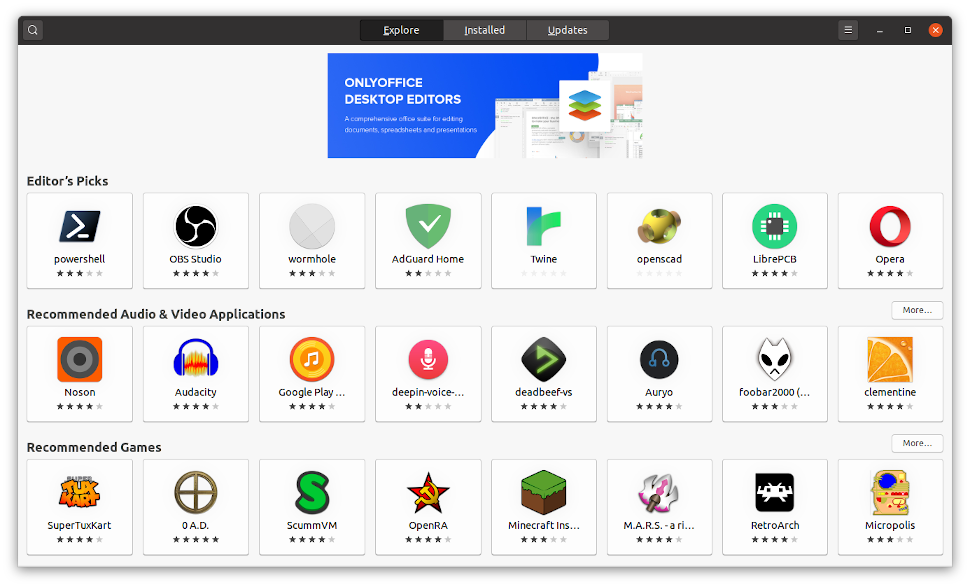
\includegraphics[scale=0.4]{cap02/loja.png}
 \caption{Ubuntu Software}
\end{figure}

Essa loja foi um dos melhores softwares criados nos últimos anos para Linux (e um grande avanço em relação a versões anteriores). Podemos dizer que foi a concretização do projeto original sobre os ``APT do Debian'' e buscava substituir por completo a instalação através da tela de terminal, além de ter uma espécie de ``supermercado de aplicativos'', no qual se escolhe, clica e instala. A instalação de um aplicativo é equivalente no terminal ao comando: \\
{\ttfamily\$ sudo apt install [nome-aplicativo]} 

No mundo dos derivados do Debian, existem os aplicativos com a extensão \textbf{.deb}\footnote{Para instalar este tipo de arquivo é necessário primeiramente instalar o \textbf{GDebi}, que pode ser localizado na loja} (que funcionam como se fossem os \textbf{.exe} do Windows) e esses arquivos permitem a instalação de softwares de terceiros sem ter que adicionar um repositório.
\\[3mm]
\begin{dica}[Sudo] Tenha sempre em mente que no mundo Linux existem dois usuários bem distintos, o seu usuário e o superusuário, e apenas para esse segundo que é permitido instalar ou remover aplicativos, então tenha sempre a mão a senha desse superusuário, que foi definida ao se instalar o sistema operacional.
\end{dica}
Para desinstalar quaisquer aplicativo no Ubuntu basta realizar essa ação através da Loja, ou conhecendo o nome correto do programa, digitar o seguinte comando no terminal: \\
{\ttfamily\$ sudo apt remove [nome-aplicativo]}

Como alternativa\footnote{Prefiro mais pensar na palavra: \textbf{complemento}} a loja, os usuários gostam de instalar o \textbf{Synaptic} que é um gerenciador de repositórios. Use-o com maior cuidado e atenção, pois assim que entramos nesse aplicativo a senha do superusuário deve ser informada, então o aplicativo possui o poder de realizar qualquer ação no seu sistema, inclusive a de remover pacotes que podem danificá-lo.

\section{Adicionar e Remover Repositórios}\index{Falando com Ubuntu}
Onde estão os aplicativos instalados através da loja? Se encontram na Internet em um endereço que para o sistema é conhecido como \textbf{Repositório}. Alguns repositórios são colocados por padrão no seu sistema, enquanto que outros devem ser adicionados.

Para adicionar um repositório os usuários comumente utilizam o terminal (inclusive em muitos sites é muito comum encontrar essa sintaxe), composta por dois comandos: \\
{\ttfamily\$ sudo add-apt-repository ppa:[Nome\_PPA]/ppa}

Venho frisando, desde o início deste livro, que possuo o desejo de tornar as coisas mais fáceis, então em vez de abrir um terminal para realizar este processo, acesse o \textbf{PA} e na aba \textbf{Outros Programas} e teremos a seguinte visão:
\begin{figure}[H]
 \centering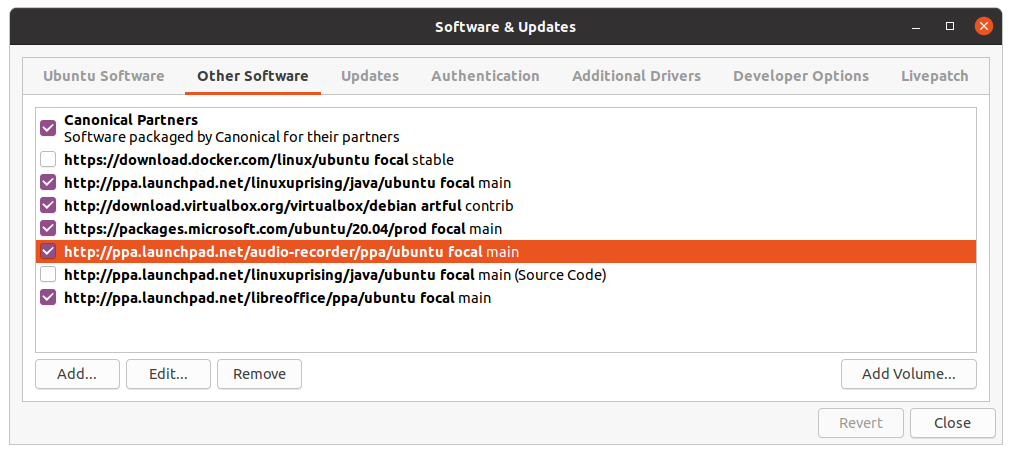
\includegraphics[scale=0.4]{cap02/outrosProgramas.png}
 \caption{Programas e atualizações, aba Outros Programas}
\end{figure}

Pessoalmente acho que essa aba deveria se chamar Repositórios, pois aí se localiza todos os repositórios disponibilizados pelo sistema. Ou seja, basta pressionar o botão \textbf{Adicionar...} e informar o local aonde está o repositório, com a seguinte sintaxe: \\
{\ttfamily deb http://ppa.launchpad.net/[Nome\_PPA]/ubuntu [codinome] main}

Por exemplo, um repositório que está na versão \textbf{Ubuntu 14.10} seria assim adicionado: \\
{\ttfamily deb http://ppa.launchpad.net/[Nome\_PPA]/ubuntu utopic main}

Note que apenas o substantivo do codinome da versão é usado. Ao fechar o aplicativo o equivalente ao comando do terminal é executado: \\
{\ttfamily\$ sudo apt update}

Para eliminar um repositório, basta localizá-lo e clicar no botão Remover. Isso corresponde ao seguinte comando do terminal: \\
{\ttfamily\$ sudo add-apt-repository ---remove ppa:[Nome\_PPA]}

Essa lista de repositórios, que visualizamos no aplicativo, também pode ser vista no terminal com o seguinte comando: \\
{\ttfamily\$ sudo ls /etc/apt/sources.list.d}

Com o repositório instalado basta ir na Loja e pesquisar pelo nome do aplicativo e instalá-lo sem maiores dificuldades, então quando, neste livro, houver a necessidade de instalar um repositório para um aplicativo apenas indicarei qual a composição do nome do repositório a instalar: \vspace{-1em}
\begin{itemize}[noitemsep]
 \item Repositório: [Nome\_PPA]
 \item Aplicativo: [Nome\_Aplicativo]
\end{itemize}

\subsection{E se um repositório não for reconhecido?}\index{Falando com Ubuntu}
Duas coisas podem ter acontecido, primeira o nome do repositório foi digitado incorretamente (verifique se o nome é realmente este) ou este repositório é incompatível com a versão do Ubuntu utilizada, neste caso não é recomendável a instalação do aplicativo (que pode ser forçada através dos comandos do terminal por sua conta e risco). Exatamente por este motivo que recomendo ao usuário leigo o uso da parte gráfica como forma de controlar melhor seus repositórios.

No caso de alguns softwares pode ocorrer que não apareça na loja pois esta não trabalha com qualquer repositório (que pode ser um de terceiro), então obrigatoriamente devemos instalá-lo a partir do terminal com o comando: \\
{\ttfamily\$ sudo apt install [nome]}

\subsection{Snappy – Um novo modelo de aplicativos}\index{Falando com Ubuntu}
O Ubuntu 16.10 trouxe o início de uma profunda mudança que é a disponibilização de um novo modelo de pacotes denominados Snappy (ou Snap\footnote{Snap pode ser traduzido para romper ou arrebentar, mas o sentido mais comum e estalo ou ruptura} como estão sendo apelidados). A grande vantagem deste novo modelo é a palavra ``Convergência'', no qual um mesmo pacote pode ser instalado em vários hardwares que contenham a versão do sistema operacional (desktop, tablets, celulares, e por aí vai). Seu uso ainda é modesto e centralizado (assim como no início dos pacotes APT) no terminal ou através da Internet no seguinte endereço \url{https://snapcraft.io/store}.

Encontrar os pacotes disponíveis: \\
{\ttfamily\$ snap find [aplicativo]}

Obter informações de algum pacote: \\
{\ttfamily\$ snap info [aplicativo]}

Instalar algum pacote: \\
{\ttfamily\$ sudo snap install [aplicativo]}

Verificar os pacotes que estão instalados no sistema: \\
{\ttfamily\$ snap list}

Obter um histórico das mudanças dos pacotes no sistema: \\
{\ttfamily\$ snap changes}

Realizar um upgrade para a nova versão: \\
{\ttfamily\$ sudo snap refresh [aplicativo]}

Remover um pacote: \\
{\ttfamily\$ sudo snap remove [aplicativo]}

Se é desenvolvedor, caso possua e deseja logar na conta do Ubuntu One: \\
{\ttfamily\$ sudo snap login [email]}

A Canonical está pressionando para torná-los um novo padrão ao Ubuntu e assim poder disponibilizar a Convergência. Foi lançada uma ferramenta chamada de \textbf{Snapcraft} de modo que será mais fácil os desenvolvedores criarem novos aplicativos em várias linguagens de programação. Acesse o site para descobrir vários pacotes que está a disposição neste novo formato: \url{https://uappexplorer.com/apps?type=snappy}

\subsection{Resumindo tudo e AppImage}\index{Falando com Ubuntu}
Então o que sabemos sobre os aplicativos do Ubuntu é que eles podem ser de três tipos: \vspace{-1em}
\begin{enumerate}[noitemsep]
 \item Pacote \textbf{deb}, que contém o aplicativo completo sem a necessidade de instalar um repositório.
 \item Pacote \textbf{snappy}, que também contém o aplicativo completo sem a necessidade de instalar um repositório.
 \item Aplicativo comum que pode ou não ter a necessidade de instalar um repositório extra.
\end{enumerate}

E como se nada disso fosse suficiente uma quarta forma está surgindo é chamada de \textbf{AppImage}, nesse formato não é necessário instalar absolutamente nada no seu sistema basta apenas baixar o arquivo, transformá-lo em um executável e clicar nele. Vamos tentar entender como isso funciona com um excelente software editor de partituras, acesse o site oficial em \url{https://musescore.org/pt-br/download}, localize e baixe a AppImage.

Abra o Nautilus (Gerenciador de Arquivos), localize a pasta /Downloads e clique com o botão direito do mouse sobre o arquivo baixado e acesse a aba \textbf{Permissões}. Marque a opção ``Permitir a execução do arquivo como um programa'', saia da tela e simplesmente clique no arquivo que o programa \textbf{MuseScore} será aberto sem ser realizada nenhuma instalação no seu sistema. 
\begin{figure}[H]
 \centering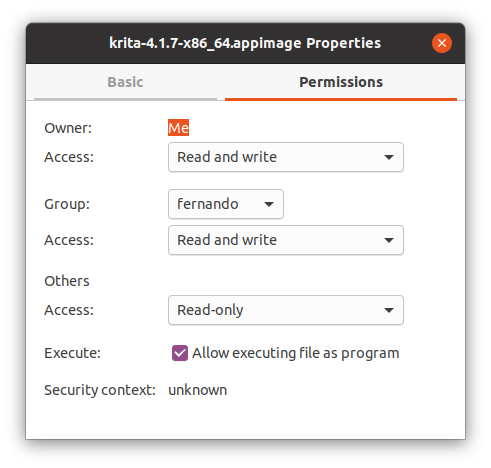
\includegraphics[scale=0.4]{cap02/executavel.png}
 \caption{Propriedades, aba Permissões}
\end{figure}

Calma que o mundo não é assim tão maravilhoso, a vantagem bem clara que é possível criar uma pasta e colocar diversos aplicativos nela sem ter que instalar (e sujar) absolutamente nada no seu sistema. Porém a desvantagem seria mais relacionada a atualização do aplicativo como não existe um repositório e esse arquivo está ``estável'' em seu sistema e não existirá a atualização do mesmo. Então minha recomendação é: \textit{use este tipo de pacote para testar um aplicativo, gostou e vai realmente usá-lo? Instale-o}.

\section{Atalhos ou Lançadores}\index{Falando com Ubuntu}
Uma das grandes diferenças entre os sistemas Windows e Linux é em relação aos Lançadores (\textbf{Atalhos} é coisa de Windows). No Windows são arquivos misteriosos que pouca gente sabe seu conteúdo, sabe simplesmente que se clica com o botão direito sobre um executável (aqui não existe esse conceito) e seleciona a opção ``Criar atalho'' então a mágica acontece. 

No Linux são arquivos com a extensão \textbf{.desktop} e que possuem a permissão de serem executados pelo sistema (uma vez que estão corretamente definidos). Residem na pasta /usr/share/applications (o Dash só reconhece as aplicações que estão nesta pasta), mas para um usuário que vem do Windows a primeira tendência é a de copiar um punhado deles para a \textbf{Área de Trabalho}.

Esses arquivos possuem uma estrutura definida, vejamos como exemplo o lançador que chama o aplicativo que controla o \textbf{Brilho \& Bloqueio}:
\begin{lstlisting}
[Desktop Entry]
Name=Brightness & Lock
Comment=Screen brightness and lock settings
Exec=unity-control-center screen
Icon=system-lock-screen
Terminal=false
Type=Application
Categories=GNOME;GTK;Settings;DesktopSettings;X-Unity-Settings-Panel
\end{lstlisting}

Observamos que é quase um arquivo auto explicativo (retirei algumas variáveis desnecessárias a fim de visualizarmos melhor o arquivo) e a única coisa que devemos ter em mente é que a variável \textbf{Exec} chamará o aplicativo, sendo que o comando colocado aqui seria o seu equivalente a tela de terminal. E um lançador estará criado pois as outras variáveis são simples informações. Recomendo que use este arquivo como um modelo para criar seus próprios lançadores quando houver necessidade.

\subsection{Entre o Nano e o gEdit}\index{Falando com Ubuntu}
A briga entre o ambiente gráfico e não gráfico é muito estranha, vamos comparar esses dois editores. Várias vezes precisamos editar arquivos que não podem ganhar ``caracteres estranhos'' como os colocados por aplicativos como Writer (LibreOffice) ou MS-Word (MS-Office), assim precisamos utilizar de editores mais simples, no Windows seria o equivalente ao ``Bloco de Notas''.

Existem para o ambiente Linux dois excelentes editores: \textbf{Nano} e \textbf{gEdit}, a diferença? O primeiro não é gráfico e o segundo totalmente gráfico. Abra uma janela de terminal e digite o comando: \\
{\ttfamily\$ nano}

E a seguinte tela será chamada:
\begin{figure}[H]
 \centering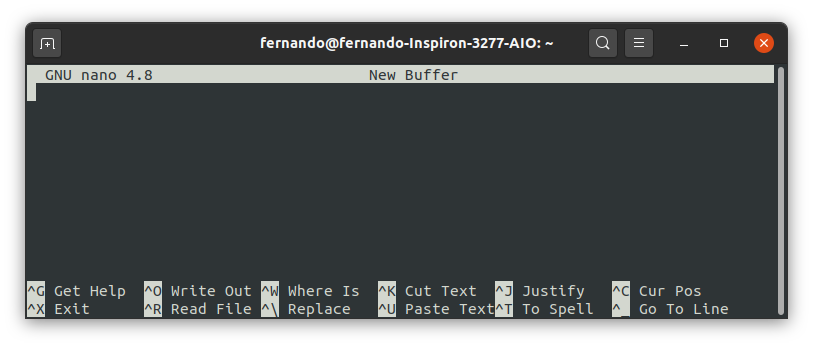
\includegraphics[scale=0.4]{cap02/nano.png}
 \caption{Editor Nano}
\end{figure}

Os comandos do editor estão expostos na barra do rodapé, sendo que o caractere circunflexo corresponde a tecla \textbf{Ctrl}, ou seja, para gravar pressionamos \textbf{Ctrl + O}, sair do editor \textbf{Ctrl + X} e assim sucessivamente. Outro detalhe interessante é possível pará-lo, retornar ao terminal, proceder alguma ação e retornar ao editor. Isso é chamado de Job (trabalho). Guarde bem os seguintes comandos: \vspace{-1em}
\begin{itemize}[noitemsep]
 \item No nano pressione \textbf{Ctrl + Z} para parar o job.
 \item No terminal escreva: {\ttfamily jobs}, para ver os jobs que estão parados. 
 \item No terminal escreva: {\ttfamily fg [n]}, para retornar a um job parado. 
\end{itemize}

Já o gEdit, por ser um programa gráfico, pode ser acessado de três maneiras diferentes: \vspace{-1em}
\begin{enumerate}[noitemsep]
 \item Abrir o aplicativo ``Editor de Textos'' no Dash
 \item Pressionar \textbf{Alt + F2} e digitar {\ttfamily gedit}
 \item Através do seguinte comando no terminal: {\ttfamily\$ gedit}.
\end{enumerate}

O efeito será o mesmo e a seguinte tela será mostrada:
\begin{figure}[H]
 \centering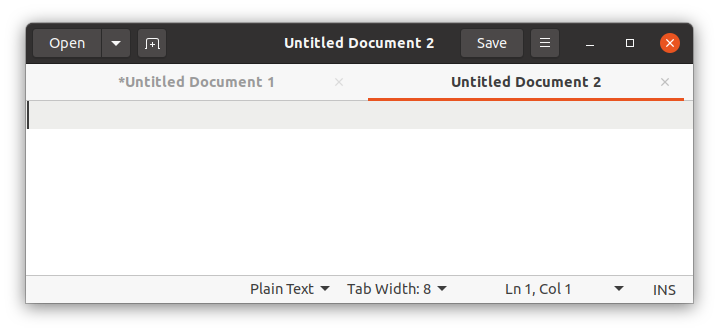
\includegraphics[scale=0.4]{cap02/gedit.png}
 \caption{Editor gEdit}
\end{figure}

Ou seja, trabalhar com um ou outro torna-se apenas uma questão de gosto pessoal. Porém, pode existir o caso do ambiente gráfico não estar presente e assim o Nano acaba por tornar a única ponte de salvação para a edição dos arquivos, a menos que prefira algo como \textbf{Vi} que já disse se tratar da obra do Demônio.

\subsection{Entre o chmod e o Nautilus}\index{Falando com Ubuntu}
Meio estranho dizer isso no título pois um deles é apenas um simples comando para modificar as permissões de um arquivo enquanto que o outro é um gerenciador de arquivos. No Nautilus basta clicar com o botão direito sobre qualquer arquivo e acessar a aba \textbf{permissões}. 

Ou então entrar no terminal e digitar (em qualquer pasta que existam arquivos) o seguinte comando: \\
{\ttfamily\$ ls -l}

Na listagem dos arquivos (logo na primeira coluna) aparecerá algumas letras, entre elas: d, r, w e x. Estas letras são permissões e se divide nos seguintes grupos: Dono (ou proprietário), Grupo e Outros. As letras podem ser: \vspace{-1em}
\begin{itemize}[noitemsep]
 \item r – listar o conteúdo de pastas ou ler arquivos
 \item w – gravar em arquivos ou  pastas
 \item x – recursivo na árvore de pastas
 \item X – execução
 \item s – novos arquivos ou diretórios
 \item d – indicação de pasta
 \item Não aparecer a letra – herança da pasta
\end{itemize}

Porém o comando \textbf{chmod} também permite que façamos as trocas dessas permissões através do terminal, sua formação é realizada pelas letras ou por valores. Esse são os seguintes: \vspace{-1em}
\begin{itemize}[noitemsep]
 \item 0 – nada
 \item 1 – execução
 \item 2 – gravação
 \item 4 – leitura
\end{itemize} 

O somatório dos números também é válido, ou seja, para dar permissão de leitura e gravação usamos o número 6, já leitura e execução o 5 e assim sucessivamente. Por exemplo para dar permissão completa a um arquivo, podemos digitar o seguinte comando: \\
{\ttfamily\$ chmod 0777 nomearquivo}

O que é esse primeiro número? A informação deve ser passada em base Octal, e essa começa por 0. Para usarmos as letras, o sinal de soma (+) adiciona uma permissão, enquanto que o sinal de subtração (-) remove a permissão, então o mesmo comando poderia ser descrito da seguinte forma: \\
{\ttfamily\$ chmod a+rwx nomearquivo}

O significado é que o primeiro ``a'' é uma notação que indica modo de adição dos valores, podemos também usar ``i'' que indica imutabilidade ou ``s'' indicando segurança para exclusão. Quando usar um ou outro? Tanto faz, normalmente o que ficar mais simples. Por exemplo, para dar permissão de leitura e gravação para o usuário, apenas leitura para o grupo e outros. Para utilizar números resolvemos assim: \\
{\ttfamily\$ chmod 0644 nomearquivo}

Já com letras deveriamos realizar vários comandos para conseguirmos isso. Já para dar permissão de execução (por exemplo a um Script), bastaria digitar: \\
{\ttfamily\$ chmod +x nomearquivo}

Permissões em arquivos ou pastas são muito importantes, recomendo que aprenda as duas formas de trabalhar pois, como disse, nunca se sabe quando o terminal se tornar a única opção.

% Final do Capítulo
\clearpage
% EDA
% %------------------------------------------------------------------------------------
%	CHAPTER 3
%------------------------------------------------------------------------------------
\chapterimage{headConceito.png}
\chapter{EDA}

\begin{remark}
Nós torturamos os dados até eles confessarem. (Ricado Cappra - Cientista de Dados) 
\end{remark}

\section{Passos da EDA}\index{EDA}
EDA é fundamental para entender qualquer conjunto de observações. É aqui podemos obter informações e fazer descobertas. Aqui colocamos o conhecimento para trabalhar. Acrônimo para \textit{Exploratory Data Analysis} (Análise Exploratória de Dados), desempenha um papel crítico na compreensão do quê? por que? e como? na declaração do problema. 

É a primeira ação realizada na ordem das operações que um Cientista de Dados deve executar ao receber uma nova fonte de observações e a declaração de problema. Tratamos EDA como uma série de técnicas utilizadas como forma de entendermos os diversos aspectos que temos para trabalhar.
\begin{figure}[H]
	\centering
	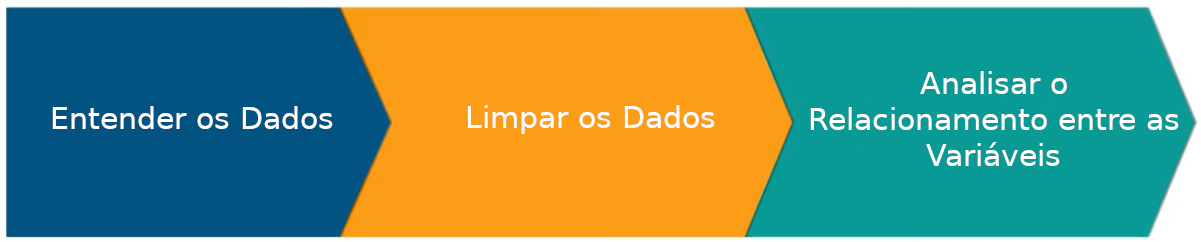
\includegraphics[width=0.6\textwidth]{cap03/EDA.png}
	\caption{Passos da EDA}
\end{figure}

A preparação dos dados para análise é inevitável, e a maneira como fazemos isso define a sua qualidade. Na prática o que faremos nesse capítulo é compreendermos o que temos a nossa disposição para trabalhar.

Normalmente as observações se dividem em atributos \textbf{Preditores} (Entradas) e \textbf{Alvo} (saída). Uma vez que os localizemos, devemos identificar seu tipo e categoria.

\section{Passo 1 - Entender os Dados}\index{EDA}
Nesta fase precisamos compreender o que temos a nossa disposição. Começamos o processo com a importação das bibliotecas:
\begin{lstlisting}[]
import pandas as pd
import matplotlib.pyplot as plt
import seaborn as sns
%matplotlib inline
\end{lstlisting}

Vamos trabalhar com três bibliotecas básicas, que como já mencionamos devemos conhecê-las a fundo: \textbf{Pandas} para análise, \textbf{MatPlotLib} e \textbf{SeaBorn} para mostrar em forma gráfica.

Agora precisamos dos dados, para isso usaremos o arquivo \textit{StudentsPerformance.csv}:
\begin{lstlisting}[]
df = pd.read_csv('StudentsPerformance.csv')
\end{lstlisting}

Nessa fase compreendemos melhor o que temos na nossa mão, \textbf{Pandas} é ideal para essa tarefa. Seu funcionamento é como um "Editor de Planilha", dessa forma que devemos encarar essa biblioteca, sua diferença básica é a nomenclatura de como o \textit{DataFrame} (e não Planilha) é visualizado:
\begin{figure}[H]
	\centering
	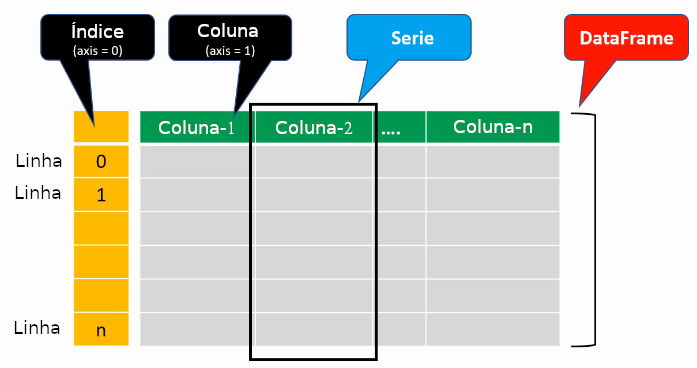
\includegraphics[width=0.7\textwidth]{cap03/PandasData.png}
	\caption{Visão Pandas}
\end{figure}

Uma coluna aqui é vista como uma \textit{Serie} e \textit{index} é o que mantêm a "cola" das series juntas. Dois comandos são básicos para visualizarmos o \textit{DataFrame}:
\begin{lstlisting}[]
df.head()
\end{lstlisting}

Porém nesse livro não utilizaremos o termo "coluna" e sim "atributo" (consideremos ambos como sinônimos). Mostra as primeiras observações, como parâmetro podemos passar a quantidade. E:
\begin{lstlisting}[]
df.tail()
\end{lstlisting}

Mostra as últimas observações e também como parâmetro podemos passar a quantidade. O que temos até o momento? Sabemos é uma base sobre estudantes e as linhas são: gênero, etnicidade, nível de escolaridade dos pais, forma de alimentação, realizou um teste de preparação do curso, nota de matemática, nota de leitura e nota de escrita.

Então só com esses dois comandos já podemos saber sobre qual assunto iremos tratar: estudantes que realizaram provas e em quais condições. Quantos registros temos a nossa disposição? Ou quais são os nomes dos atributos?
\begin{lstlisting}[]
print("Tamanho: ", df.shape)
print("Nome dos Atributos: ", df.columns)
\end{lstlisting}

As variáveis \textit{shape} e \textit{columns} do \textit{DataFrame} respondem aos questionamentos. De forma mais completa podemos usar:
\begin{lstlisting}[]
df.info()
\end{lstlisting}

Nos mostra inclusive o tipo de cada atributo e se contém ou não elementos nulos. Temos 3 atributos que são do tipo inteiro (\textit{int64}) e podemos analisá-los com o comando:
\begin{lstlisting}[]
df.describe()
\end{lstlisting}

Nos fornece as informações estatísticas básicas como média, desvio padrão, menor valor, máximo, 1º quartil (25\%), 2º quartil ou mediana (50\%), 3º quartil (75\%) e o maior valor. Ou seja, as informações para a montagem de um \textbf{BoxPlot}. Vamos montá-lo para melhor visualizar as observações:
\begin{lstlisting}[]
fig, axes = plt.subplots(1, 3, figsize=(10,4))
axes[0].boxplot(df['math score'])
axes[0].set_title("Matemática")
axes[1].boxplot(df['reading score'])
axes[1].set_title("Leitura")
axes[2].boxplot(df['writing score'])
axes[2].set_title("Escrita")
plt.show()
\end{lstlisting}

E obtemos como resultado:
\begin{figure}[H]
	\centering
	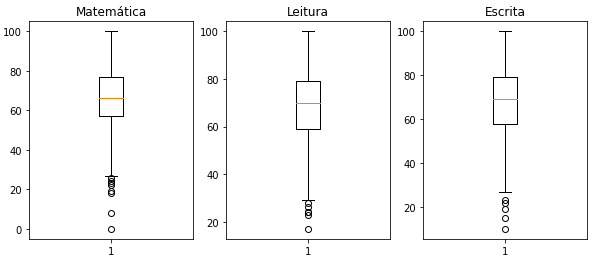
\includegraphics[width=0.55\textwidth]{cap03/BoxPlot.png}
	\caption{BoxPlot das Notas}
\end{figure}

\textbf{Boxplot}\footnote{Diagrama de Caixa se prefere, foi atribuída ao matemático \textbf{John W. Tukey} (1915 –2000), curiosamente algumas literaturas chamam de "\textit{Tukey BoxPlot}", mas se realizar uma pesquisa ninguém sabe ao certo quem criou realmente esse diagrama.} é um gráfico que avalia a distribuição das observações. É formado exatamente com os atributos que mostramos na função \textit{describe()}. Porém suas hastes (inferiores e superiores) se estendem do quartil inferior (ou superior) até o menor valor não inferior (ou superior) ao limite. São calculados da seguinte forma: \vspace{-1em}
\begin{itemize}
	\item Limite inferior: $Q_1 - 1,5 \times (Q_3 - Q_1)$.
	\item Limite superior: $Q_3 + 1,5 \times (Q_3 - Q_1)$.
\end{itemize}

Resumidamente é formado da seguinte maneira:
\begin{figure}[H]
	\centering
	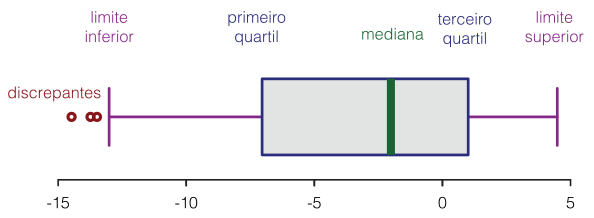
\includegraphics[width=0.6\textwidth]{cap03/estrutBoxplot.png}
	\caption{Estrutura do BoxPlot}
\end{figure}

Esses pontos "discrepantes" podem ocorrer acima ou abaixo dos limites, são chamados de \textit{Outliers}. Não é necessariamente um erro, podemos classificá-lo como uma anomalia curiosa e que merece nossa atenção.

\subsection{Localizar os Outliers}\index{EDA}
Para achar esses \textit{Outliers} isolamos os três atributos numéricos:
\begin{lstlisting}[]
X = df.iloc[:, 5:8].values
\end{lstlisting}

E criamos um novo \textit{DataFrame} somente com a modificação de nome por um número:
\begin{lstlisting}[]
pd.options.display.float\_format = '{:.1f}'.format
xDF = pd.DataFrame(X)
\end{lstlisting}

Para quê isso serve? A função \textit{describe()} cria um \textit{DataFrame}, podemos percorrê-lo, porém fica muito mais simples se cada atributo for um numeral, pois assim podemos usar um comando \textit{for} para isso:
\begin{lstlisting}[]
z = xDF.describe()
for t in z:
  iqr = z[t][6] - z[t][4]
  extMenor = z[t][4] - (iqr * 1.5)
  extMaior = z[t][6] + (iqr * 1.5)
  print('Para o índice \%d valores devem estar abaixo de \%.2f e acima de \%.2f' \% (t, extMenor, extMaior))
\end{lstlisting}

E obtemos o seguinte resultado: \\
\codigo{Para o índice 0 valores devem estar abaixo de 27.00 e acima de 107.00 \\
Para o índice 1 valores devem estar abaixo de 29.00 e acima de 109.00 \\
Para o índice 2 valores devem estar abaixo de 25.88 e acima de 110.88}

Pelo BoxPlot todos os valores estão abaixo, então para localizá-los:
\begin{lstlisting}[]
matOutliers = (X[:,0] < 27)
df[matOutliers]
\end{lstlisting}

E assim mostramos todas as observações que a nota de matemática (índice 0) é abaixo do valor 27. Proceder de mesmo modo para as notas de leitura (índice 1) e escrita (índice 2) e assim desvendar quais são os \textit{Outliers}.

Podemos também analisar graficamente e visualizar a Distribuição Normal de cada atributo, por exemplo para a nota de Escrita:
\begin{lstlisting}[]
sns.kdeplot(df['writing score'], shade=True)
plt.show()
\end{lstlisting}

Obtemos como resultado:
\begin{figure}[H]
	\centering
	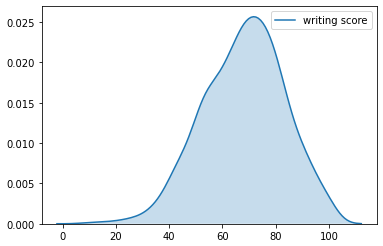
\includegraphics[width=0.5\textwidth]{cap03/NotaEscrita.png}
	\caption{Distribuição das observações para Nota de Escrita}
\end{figure}

E assim verificamos como cada atributo numérico se comporta.

\subsection{Tratar Atributos Categóricos}\index{EDA}
Sabemos que os primeiros cinco atributos do \textit{Dataframe} são categóricos, porém conforme a função \textit{info()} o tipo delas estás \textit{object}. É interessante mudarmos para o tipo caractere para evitarmos quaisquer problemas futuros.
\begin{lstlisting}[]
df['gender'] = df['gender'].astype(pd.StringDtype())
df['race/ethnicity'] = df['race/ethnicity'].astype(pd.StringDtype())
df['parental level of education'] = df['parental level of education'].astype(pd.StringDtype())
df['lunch'] = df['lunch'].astype(pd.StringDtype())
df['test preparation course'] = df['test preparation course'].astype(pd.StringDtype())
\end{lstlisting}

E ao aplicarmos uma nova chamada a função \textit{info()} vemos que os tipos agora estão corretos. Quantos tipos únicos existem para cada atributo?
\begin{lstlisting}[]
df.nunique()
\end{lstlisting}

Mostra a quantidade de valores não repetidos de cada atributos (inclusive os numéricos). E agora sabemos que temos: 2 gêneros, 5 etnicidades, 6 níveis de escolaridade dos pais, 2 formas de alimentação e 2 tipos para teste de preparação do curso. Mas quem são?
\begin{lstlisting}[]
print("Gênero: ", df['gender'].unique())
print("Etinicidade: ", df['race/ethnicity'].unique())
print("Escolaridade dos Pais: ", df['parental level of education'].unique())
print("Refeição: ", df['lunch'].unique())
print("Realizou Preparatório: ", df['test preparation course'].unique())
\end{lstlisting}

\section{Passo 2 - Limpar os Dados}\index{EDA}
A limpeza dos dados trata de muitos problemas como informação repetida, valores faltantes (que podem ser descobertos por associação) e inconsistentes. Para esse último tipo o pior caso são os nulos. (In)felizmente essa base está horrível para essa fase e assim pegamos um outro arquivo \textbf{titanic.csv}: 
\begin{lstlisting}[]
df = pd.read_csv('titanic.csv')
df.head()
\end{lstlisting}

Repetimos todo o processo da fase anterior para descobrirmos de que se tratam as observações e descobrimos que são os passageiros (sobreviventes ou não - atributo \textit{Survived} - sendo este atributos alvo) do famoso \textbf{RMS Titanic}, este foi pensado para ser o navio mais luxuoso e seguro de sua época e supostamente "inafundável". Como sabemos em sua viagem inaugural de \textit{Southampton} para \textit{Nova Iorque} afundou no dia 14 de abril de 1912 com mais de 1.500 pessoas a bordo. Porém esta base contém apenas 891 registros.

Ao aplicarmos a função info() percebemos que os atributos \textit{Age} (idade), \textit{Cabin} (número da cabine) e \textit{Embarked} (local de Embarque) possuem valores faltantes. Que valores são esses?
\begin{lstlisting}[]
print(df.isnull().sum())
\end{lstlisting}

Sabemos que faltam: 177 em \textbf{Age}, 687 em \textbf{Cabin} e 2 em \textit{Embarked}. Também podemos mostrar exclusivamente os que faltam, isso é útil para quando temos muitos atributos no modelo:
\begin{lstlisting}[]
null_value_stats = df.isnull().sum(axis=0)
null_value_stats[null_value_stats != 0]
\end{lstlisting}

Ou ainda criar uma função personalizada que retorna um \textit{Dataframe} com a informação mais completa o possível (inclusive com seu percentual):
\begin{lstlisting}[]
def mostrarNulos(data):
  null_sum = data.isnull().sum()
  total = null_sum.sort_values(ascending=False)
  percent = (((null_sum / len(data.index))*100).round(2)).sort_values(ascending=False)
  df_NULL = pd.concat([total, percent], axis=1, keys=['Tot.Nulo', 'Perc.Nulo'])
  df_NULL = df_NULL[(df_NULL.T != 0).any()]
  return df_NULL
\end{lstlisting}

E ao chamá-la:
\begin{lstlisting}[]
df_Age = mostrarNulos(df)
df_Age.head()
\end{lstlisting}

Obtemos como resultado:
\begin{figure}[H]
	\centering
	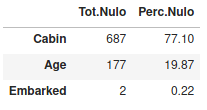
\includegraphics[width=0.3\textwidth]{cap03/TitanicNulosPerc.png}
	\caption{Nulos e Percetual da Base Titanic}
\end{figure}

Lidar com esses tipos de nulos é complicado pois não temos como consultar e o máximo que podemos fazer é podá-los da nossa base ou atribuir um valor genérico que não afete nosso resultado (como o caso de \textit{Embarked}). Porém \textbf{Número da Cabine} é um dado relevante? Essa é a principal pergunta que nos devemos fazer, por exemplo existe algum modelo preditivo que possa nos dizer que se estivéssemos em determinada cabine no navio sobreviveríamos ou não? Entretanto \textbf{Idade} é um dado relevante (lembra da frase: mulheres e crianças primeiro), então essa é uma característica que pode ser essencial.

Criar uma função com um gráfico para mostrar, por idade, como estão as observações:
\begin{lstlisting}[]
def executarGrafico():
  try:
    sns.distplot([df['Age']])
    plt.show()
  except ValueError as err:
    print(err) 
\end{lstlisting}

Agora a cada vez que chamarmos essa função obtemos como resultado:
\begin{figure}[H]
	\centering
	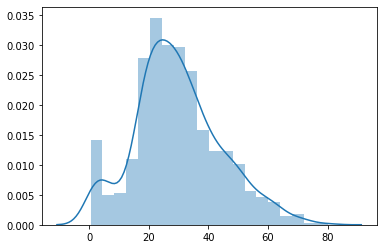
\includegraphics[width=0.45\textwidth]{cap03/TitanicIdade1.png}
	\caption{Gráfico de Idade do Titanic}
\end{figure}

\begin{note}[Imputação ou retirada de valores] 
	Como tratamos de adicionar ou retirar elementos na base a cada vez devemos ler novamente as observações contidas no arquivo CSV.
\end{note}

Porém em algumas versões da \textit{SeaBorn} este pode apresentar erro devido a presença dos nulos, é ideal que os retiremos do \textit{DataFrame} para evitarmos problemas. Em muitas biografias encontramos algo do tipo: "atribuir um valor (preferencialmente \textit{outlier}) para estes tipos". Tentaremos essa técnica com os seguintes comandos:
\begin{lstlisting}[]
df['Age'].fillna(-25, inplace=True)
executarGrafico()
\end{lstlisting}

Obtemos como resultado:
\begin{figure}[H]
	\centering
	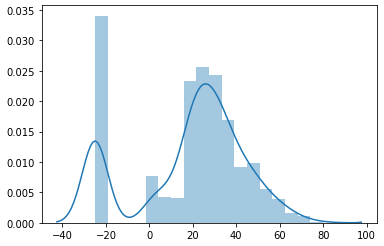
\includegraphics[width=0.45\textwidth]{cap03/TitanicIdade2.png}
	\caption{Gráfico de Idade do Titanic com Outliers}
\end{figure}

Nosso gráfico de idade ganhou uma nova barra, que sabemos com valores não existentes, também podemos atribuir qualquer outro valor como por exemplo a média:
\begin{lstlisting}[]
df['Age'] = df['Age'].fillna(df['Age'].mean())
executarGrafico()
\end{lstlisting}

Ou a mediana (função median()) que resultaria em um gráfico completamente esquisito. Sendo assim vamos cortar esses valores:
\begin{lstlisting}[]
df = df.dropna(axis=0)
executarGrafico()
\end{lstlisting}

E teremos a seguinte situação:
\begin{figure}[H]
	\centering
	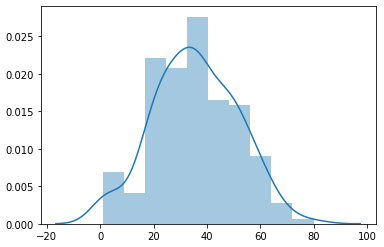
\includegraphics[width=0.45\textwidth]{cap03/TitanicIdade3.png}
	\caption{Gráfico de Idade do Titanic sem nulos}
\end{figure}

O que aconteceu? O comando executado eliminou todas as linhas que possuíam valores nulos, e o atributo \textit{Cabin} interferiu e nos deixou, conforme pode ser mostrado com a função \textit{info()}, somente 183 registros no total. Ou seja, o corte que devemos aplicar deve ser cirúrgico e somente no atributo que representa a idade.
\begin{lstlisting}[]
df['Age'] = df['Age'].dropna(axis=0)
executarGrafico()
\end{lstlisting}

O que nos resulta no mesmo gráfico mostrado no início desta e 891 registros. Como citamos, podemos retirar o atributo \textit{Cabin} para que este não interfira mais em futuras análises:
\begin{lstlisting}[]
df = df.drop(['Cabin'], axis=1)
\end{lstlisting}

\begin{note}[Ferramenta para Limpeza dos Dados] 
	Conhece o \textbf{OpenRefine?} é uma ferramenta gratuita dedicada a limpeza e tratamento das observações, baixe uma apostila gratuitamente na minha página do Academia.edu (\url{https://iesbpreve.academia.edu/FernandoAnselmo}).
\end{note}

\section{Passo 3 - Relacionamento entre os Atributos}\index{EDA}
Vamos retomar nossa base de \textbf{Estudantes} e verificarmos como os atributos se relacionam:
\begin{lstlisting}[]
df = pd.read_csv('StudentsPerformance.csv')
df.corr()
\end{lstlisting}

E temos um valor que corresponde ao grau de relacionamento, um intervalo de -1 a 1, sendo quanto mais próximo do mínimo menor é seu grau de relacionamento. Porém é muito mais fácil de visualizarmos esse resultado com um Mapa de Calor:
\begin{lstlisting}[]
rel = df.corr()
sns.heatmap(rel, xticklabels=rel.columns, yticklabels=rel.columns, annot=True)
plt.show()
\end{lstlisting}

Obtemos como resultado:
\begin{figure}[H]
	\centering
	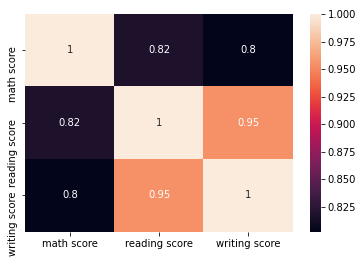
\includegraphics[width=0.5\textwidth]{cap03/MapaDeCalor.png}
	\caption{Mapa de Calor dos Relacionamentos}
\end{figure}

Vemos que as notas de Escrita e Leitura possuem um forte grau de relacionamento, como se uma fosse a responsável pela outra. Já a de matemática interfere mais na nota de leitura.

Curiosamente se aplicarmos isso na base do \textbf{Titanic} vemos que os atributos mais importantes para \textit{Fare} (sobreviveu) que é nosso alvo são: \textit{Fare} que é o valor pago pela passagem e \textit{Parch} que se refere a quantidade de pais. Ou seja, os mais ricos e se a criança tinha ou não os pais a bordo de modo a colocá-las no bote salva vidas. 

Outra maneira de visualizarmos, também de forma gráfica, é através da dispersão de valores:
\begin{lstlisting}[]
sns.pairplot(df)
plt.show()
\end{lstlisting}

Obtemos como resultado:
\begin{figure}[H]
	\centering
	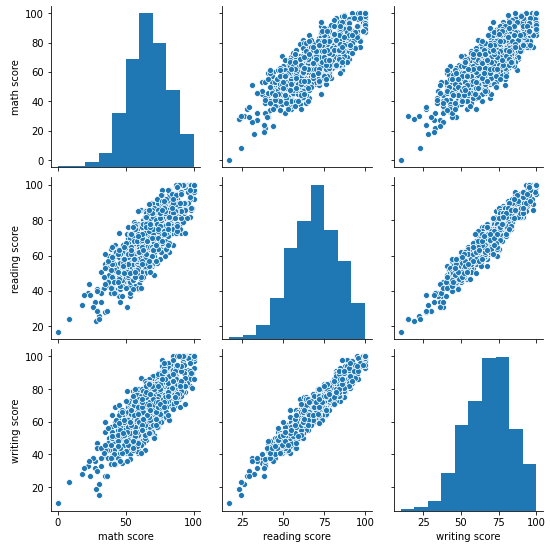
\includegraphics[width=0.7\textwidth]{cap03/dispersao.png}
	\caption{Dispersão Associada}
\end{figure}

Quanto mais juntos aparecem os pontos mais relacionadas estão. Podemos isolar as notas de Escrita e Leitura em um único gráfico, por exemplo:
\begin{lstlisting}[]
sns.regplot(x='writing score', y='reading score', data=df)
plt.show()
\end{lstlisting}

Esta função executa um ajuste e plotagem simples com base no modelo de Regressão Linear. E obtemos como resultado:
\begin{figure}[H]
	\centering
	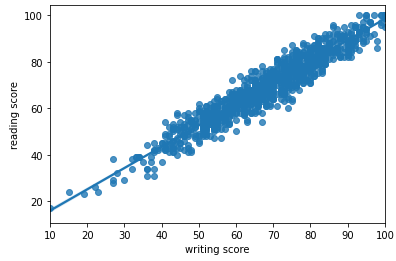
\includegraphics[width=0.55\textwidth]{cap03/NotasRegress.png}
	\caption{Notas de Leitura e Escrita}
\end{figure}

Porém o mais interessante é colorir os pontos de forma diferente com base em um atributo categórico que pode ser uma causa (para uma nota alta ou baixa), por exemplo o quanto a alimentação interferiu na nota:
\begin{lstlisting}[]
sns.lmplot(x='writing score', y='reading score', hue='lunch', data=df)
plt.show()
\end{lstlisting}

A função \textit{lmplot()} combina \textit{regplot()} com a classe \textbf{FacetGrid}. Esta auxilia visualizar a distribuição de um determinado atributos, bem como o relacionamento entre os vários separadamente dentro de subconjuntos das observações. Obtemos como resultado:
\begin{figure}[H]
	\centering
	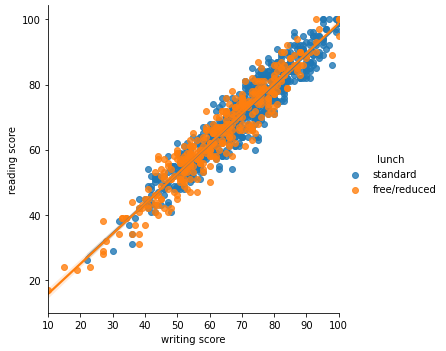
\includegraphics[width=0.5\textwidth]{cap03/NotasLmplot.png}
	\caption{Nota associada a Alimentação - RegPlot}
\end{figure}

Uma melhor forma de visualizar é usar a função \textit{relplot()} que fornece acesso a várias funções diferentes no nível de eixos que mostram o relacionamento entre dois atributos com mapeamentos semânticos de subconjuntos:
\begin{lstlisting}[]
sns.relplot(x='writing score', y='reading score', hue='lunch', data=df)
plt.show()
\end{lstlisting}

Obtemos como resultado:
\begin{figure}[H]
	\centering
	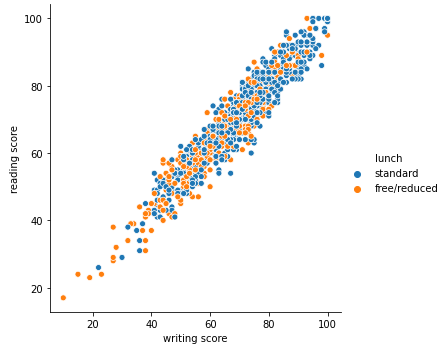
\includegraphics[width=0.55\textwidth]{cap03/NotasAlimentacao.png}
	\caption{Nota associada a Alimentação - RelPlot}
\end{figure}

Ou seja, podemos responder várias perguntas apenas com a verificação do relacionamento entre os atributos. Como forma de fixar o conhecimento procure realizar o mesmo teste com outros atributos categóricos e descobrir como se comportam em relação a nota, se existe ou não interferência.

\section{Conclusão}\index{EDA}
Mantemos em mente que EDA e um aspecto central da \textit{Data Science}, que às vezes é esquecido. O primeiro passo de qualquer ação que tomemos é conhecer as observações: entendê-las e familiarizar-se. Quais são as respostas que estamos tentando obter? Quais são os atributos e o que significam? Como é a aparência de uma perspectiva estatística? As observações estão formatadas corretamente? Possuem valores ausentes? duplicados? E quanto aos \textit{outliers}? Conhecemos eles? Ou seja, devemos responder a esses questionamentos.

É necessário muito trabalho de preparação, pois no mundo real dados raramente são limpos e homogêneos. Costumamos dizer que 80\% do tempo valioso em um Cientista de Dados é utilizado com a localização, limpeza e organização das observações. Os 20\% restantes são destinados a realizar as análises.

Agora estamos prontos para começarmos a explorar diversas observações com a utilização dos modelos.

\clearpage
% Modelos Iniciais: KNN
%------------------------------------------------------------------------------------
%	CHAPTER 4
%------------------------------------------------------------------------------------
\chapterimage{headConceito.png}
\chapter{Modelos Iniciais}

\begin{remark}
Na vida, não existe nada a temer, mas a entender. (Marie Curie - Cientista e Vencedora 2 vezes do Prêmio Nobel) 
\end{remark}

\section{K-Means}\index{Modelos Iniciais}
Acredito que K-Means seja o modelo mais simples para começarmos, este é um algoritmo de Aprendizado Não Supervisionado, ou seja, não necessita de atributos alvo para agir, sua função é de separar as observações em grupos de modo que possamos observar melhor os dados.

Sendo assim, nosso problema para usar esse algoritmo é exatamente achar esse \textbf{k} ideal de modo que os grupos sejam separados coerentemente. Para isso existe uma técnica interessante chamada "Técnica do Cotovelo" (Elbow Technique).
\begin{figure}[H]
	\centering
	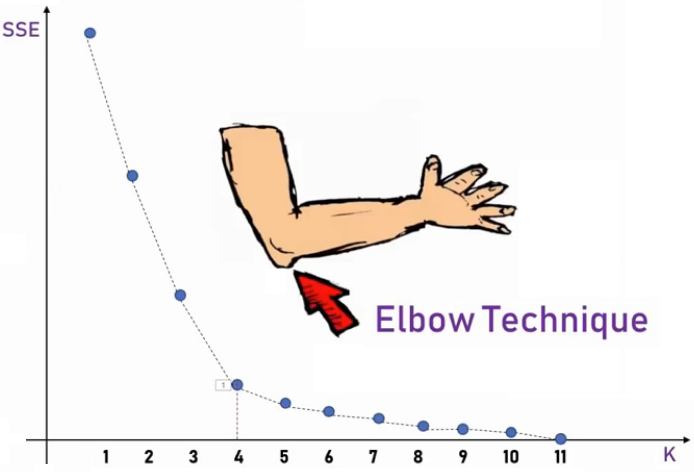
\includegraphics[width=0.46\textwidth]{cap04/tecnicaCotovelo.png}
	\caption{Técnica do Cotovelo}
\end{figure}

Exatamente na posição 4 existe uma "quebra" para passar ao próximo valor, usamos para definir essa quebra o SSE\footnote{Soma Residual dos Quadrados, é a soma dos resíduos elevado por 2. É uma medida da discrepância entre os dados e um modelo de estimativa. Um valor pequeno SSE indica um ajuste apertado do modelo aos dados.} (\textit{Sum Squared Error}).

\section{Aplicação da Técnica}\index{Modelos Iniciais}

Para achar o k ideal vamos ativar nosso JupyterLab personalizado que criamos com o Docker e na primeira célula importamos as bibliotecas necessárias:
\begin{lstlisting}[]
import pandas as pd
import numpy as np
from sklearn.preprocessing import scale
from sklearn.cluster import KMeans
from matplotlib import pyplot as plt

%matplotlib inline
\end{lstlisting}

Importamos a biblioteca Pandas e a Numpy para manipularmos os dados, a Scikit-Learn para usarmos o modelo K-Means e Matplot para vermos o resultado em um gráfico. A última linha é utilizada para mostrar os gráficos no Jupyter. Próximo passo consiste em ler os dados, baixamos o arquivo \textbf{gameML.csv} e na posição do nosso arquivo \textbf{.ipynb} criamos uma subpasta chamada \textbf{bases} e nesta colocamos o arquivo.
\begin{lstlisting}[]
df = pd.read_csv('bases/gameML.csv', delimiter=';')
df.head()
\end{lstlisting}

E como resultado da execução dessa célula devemos ter:
\begin{figure}[H]
	\centering
	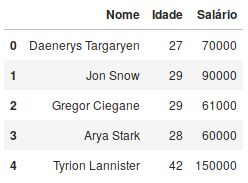
\includegraphics[width=0.4\textwidth]{cap04/baseGameML.png}
	\caption{Idades e Salários da Empresa GameML}
\end{figure}

No arquivo existem 3 campos: nome do funcionário, idade e salário, se plotarmos os dados entre idade e salário em gráfico:
\begin{lstlisting}[]
plt.scatter(df['Idade'], df['Salário'])
\end{lstlisting}

Obtemos como resultado:
\begin{figure}[H]
	\centering
	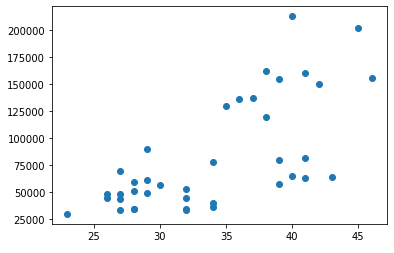
\includegraphics[width=0.55\textwidth]{cap04/plotarSalarioIdade.png}
	\caption{Idades e Salários da Empresa GameML}
\end{figure}

Quantos grupos de dados podemos distinguir? Para localizarmos a quantidade ideal aplicamos a técnica do cotovelo que consiste de:
\begin{lstlisting}[]
k_rng = range(1,10)
sse = []
for k in k_rng:
  km = KMeans(n_clusters=k)
  km.fit(df[['Idade','Salário']])
  sse.append(km.inertia_)
plt.xlabel('K')
plt.ylabel('SSE (Sum Squared Error)')
plt.plot(k_rng, sse)
\end{lstlisting}

Criar um range de 1 a 10 (um simples número máximo de possíveis \textit{clusters}), para cada valor treinamos o modelo com as variáveis e obtemos o valor do atributo \textbf{inércia}. O algoritmo agrupa dados e procura separar amostras em n grupos de igual variação, minimizando um critério conhecido como inércia ou \textbf{RSS} dentro do \textit{cluster}. O que estamos fazendo na prática e colocar o valor 1 para o \textbf{k} e guardar esse valor, em seguida o valor 2 e assim sucessivamente. Por fim plotamos esse valor em um gráfico e obtemos como resultado:
\begin{figure}[H]
	\centering
	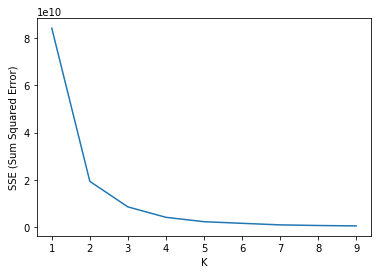
\includegraphics[width=0.53\textwidth]{cap04/aplicarCotovelo.png}
	\caption{Gráfico com os valores de Inércia}
\end{figure}

E vemos nosso "cotovelo" da curva bem na posição \textbf{3}, marcando assim o número ideal de clusters.

\section{Plotagem do Resultado do Modelo}\index{Modelos Iniciais}
Um detalhe interessante que para usarmos o algorítimo K-Means, devemos colocar os dados em "escala", vamos tentar usar o modelo sem proceder dessa forma:
\begin{lstlisting}[]
km = KMeans(n_clusters=3)
y_predict = km.fit_predict(df[['Idade','Salário']])
df['ypred'] = y_predict
df.head()
\end{lstlisting}

Já sabemos que o valor de 3 clusters é o ideal, então realizamos o treinamento com os atributos Idade e Salário para montamos um novo atributo com o resultado dessa predição (somente para que o gráfico apareça separado por cores). E plotamos o gráfico:
\begin{lstlisting}[]
cores = np.array(['green', 'red', 'blue'])
plt.scatter(x=df['Idade'],
y=df['Salário'],
c=cores[df.ypred], s=50)
\end{lstlisting}

Obtemos como resultado:
\begin{figure}[H]
	\centering
	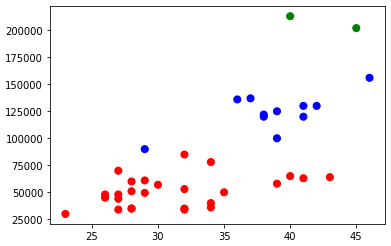
\includegraphics[width=0.55\textwidth]{cap04/separado3gruposSemEscala.png}
	\caption{Separados por Grupo}
\end{figure}

E parece que obtemos algo bem errado com alguns \textit{outliers} aparecendo, observamos o ponto azul no meio dos vermelhos e um outro azul isolado perto dos verdes. Então antes de treinarmos esse algoritmo devemos colocar os dados na mesma em escala, isso é feito assim:
\begin{lstlisting}[]
df['Salário'] = scale(df.Salário)
df['Idade'] = scale(df.Idade)
df.head()
\end{lstlisting}

Os atributos \textbf{idade} e \textbf{salário} possuem valores bem diferentes e distantes e isso gera problemas para nosso resultado final, colocar em escala e aproximar (sem modificar o resultado final) os valores seria algo criar um modelo de um prédio porém mantendo as mesmas proporções do prédio original.

A função da \textbf{Scikit-Learn} que realiza este processo é chamada \textit{scale()} e colocamos em escala os atributos se visualizarmos nossos dados agora veremos que o atributo \textbf{idade} possui valores entre -2 e 2 enquanto que \textit{salário} entre -1.5 e 3 (são diferentes exatamente para manter a proporcionalidade). Retornamos ao mesmo processo de treinamento:
\begin{lstlisting}[]
km = KMeans(n_clusters=3)
y_predict = km.fit_predict(df[['Idade','Salário']])
df['ypred'] = y_predict
df.head()
\end{lstlisting}

Plotamos novamente o gráfico e agora como resultado obtemos:
\begin{lstlisting}[]
cores = np.array(['green', 'red', 'blue'])
plt.scatter(x=df['Idade'],
y=df['Salário'],
c=cores[df.ypred], s=50)
\end{lstlisting}

E obtemos como resultado:
\begin{figure}[H]
	\centering
	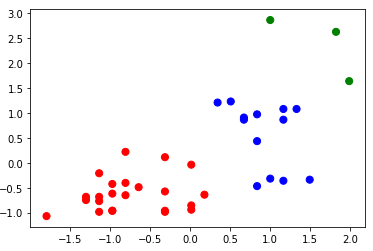
\includegraphics[width=0.55\textwidth]{cap04/separado3gruposEmEscala.png}
	\caption{Separados por Grupo em Escala}
\end{figure}

Que é um resultado bem mais coerente.

\section{K-Nearest Neighbors}\index{Modelos Iniciais}
Ou simplesmente KNN. Modelos assim existem pois muitas pessoas pensam que separar em \textit{clusters} não auxilia na predição, pois bem nosso próximo modelo é um supervisionado e destinado a Predição por Clusterização (ou se prefere por proximidade dos grupos). KNN que normalmente é usado para a predição de imagens como: Isso é um Gato? Ou não é um Gato? Porém ao invés de imagens, vamos usar uma base bem conhecida chamada \textbf{Flores Íris} para entendermos seu comportamento. 
\begin{figure}[H]
	\centering
	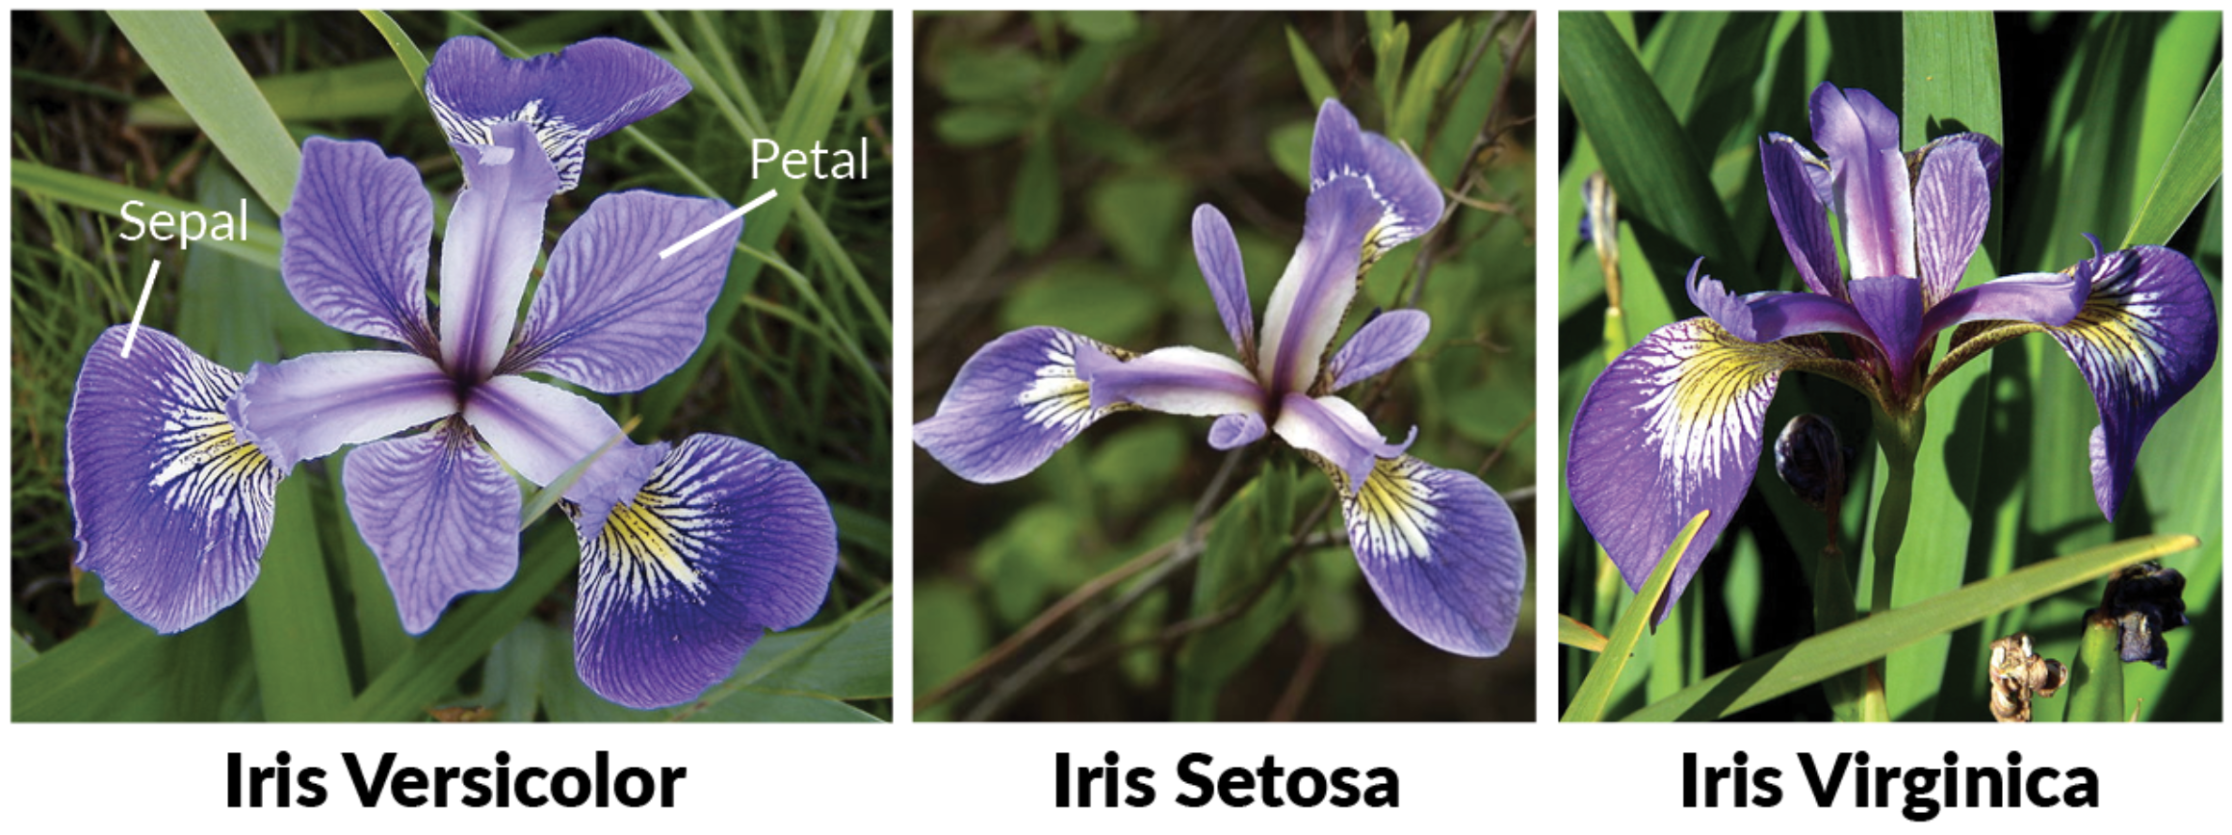
\includegraphics[width=0.65\textwidth]{cap04/iris.png}
	\caption{Flores Iris}
\end{figure}

Nessa base existem três espécies separadas: Versicolor, Setosa e Virgínica. E para distingui-las utilizamos 2 medidas da sépala e da pétala (largura e altura de cada). O problema é que algumas espécies causam as maiores confusões em nossos modelos. Para realizarmos uma predição sobre essa base importamos nossas bibliotecas:
\begin{lstlisting}[]
import numpy as np
from matplotlib import pyplot as plt
from sklearn import datasets
from sklearn.model_selection import train_test_split
from sklearn import neighbors

%matplotlib inline
\end{lstlisting}

Usamos a \textbf{NumPy} para gerenciamento dos dados. \textbf{MatPlotLib} para plotarmos os gráficos. Da \textbf{Scikit-Learn} obtemos os nossos dados através do pacote \textbf{datasets} e para separar uma massa de teste contamos com o \textit{train\_test\_split}. E a \textit{neighbors} contém o nosso algoritmo. O próximo passo consiste na preparação dos dados:
\begin{lstlisting}[]
iris = datasets.load_iris()
X, y = iris.data, iris.target

X_train, X_test, y_train, y_test = train_test_split(X, y, test_size=0.2, random_state=1234)
\end{lstlisting}

O método \textit{load\_iris()} traz a nossa base em uma matriz de dados. Nossa base está dividida em \textit{data} que contém os \textit{features} preditores (tamanho e largura da sépala e tamanho e largura da pétala, que colocaremos em X) e \textit{target}, \textit{feature} que contém a definição da espécie (0 representa \textbf{Setosa}, 1 para \textbf{Versicolor} e 2 para \textbf{Virgínica} que colocaremos em y). Usamos o método \textit{train\_test\_split} para retirar 20\% dos dados como amostra de teste e obtemos quatro agrupamentos:
\begin{itemize}[nolistsep]
	\item \textbf{X\_train}, com os dados para treino do algorítimo.
	\item \textbf{X\_test}, com os dados para teste.
	\item \textbf{y\_train}, com o resultado para o treino.
	\item \textbf{y\_test}, com o resultado para o teste.
\end{itemize}

Com nossos dados preparados vamos treinar o modelo:
\begin{lstlisting}[]
clf = neighbors.KNeighborsClassifier()
clf.fit(X_train, y_train)
print(clf.score(X_test, y_test))
\end{lstlisting}

E conseguimos uma boa acurácia com incríveis 96\% de precisão, agora é vermos na prática como isso funciona. 

\subsection{Predição com K-Nearest Neighbors}\index{Modelos Iniciais}
Primeiro vamos mostrar os dados:
\begin{lstlisting}[]
cores = np.array(['green', 'red', 'blue'])
subplt1 = plt.scatter(x=X[:, 0], y=X[:, 1], c=cores[y], s=50)
\end{lstlisting}

Pegamos as duas primeiras variáveis tamanho e largura da sépala e obtemos como resultado:
\begin{figure}[H]
	\centering
	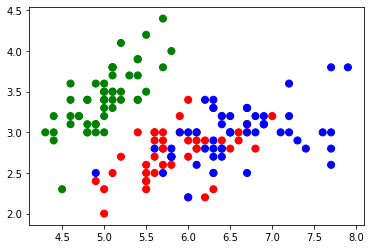
\includegraphics[width=0.5\textwidth]{cap04/knn1.png}
	\caption{Comparar tamanho e largura da Sépala}
\end{figure}

Não nos percamos nas cores \textbf{Verde} é Setosa, \textbf{Vermelho} é Versicolor e \textbf{Azul} é Virgínica. Agora vamos pensar em um ponto qualquer nesse espaço, por exemplo:
\begin{figure}[H]
	\centering
	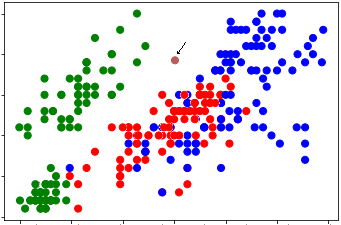
\includegraphics[width=0.5\textwidth]{cap04/acharPonto.png}
	\caption{Localizar o Ponto Roxo}
\end{figure}

O ponto roxo fica na interseção do 4º valor de X e y qual cor real ele seria? Observamos no gráfico anterior que os pontos são 6,0 e 4,0 porém nos falta o valor para mais dois atributos tamanho e largura da pétala:
\begin{lstlisting}[]
cores = np.array(['green', 'red', 'blue'])
subplt1 = plt.scatter(x=X[:, 2], y=X[:, 3], c=cores[y], s=50)
\end{lstlisting}

E obtemos como resultado:
\begin{figure}[H]
	\centering
	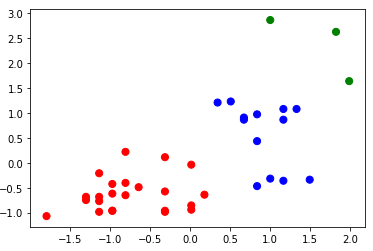
\includegraphics[width=0.55\textwidth]{cap04/separado3gruposEmEscala.png}
	\caption{Comparar tamanho e largura da Pétala}
\end{figure}

E verificamos que na interseção do 4º valor de X e y obtemos os valores 4,0 e 2,0. Agora que obtemos os quatro valores podemos realizar uma predição:
\begin{lstlisting}[]
predicao = clf.predict([[6.0, 4.0, 4.0, 2.0]])
print(predicao)
\end{lstlisting}

E resulta que o modelo prevê que é do tipo [1], ou seja, um ponto vermelho da espécie \textbf{Versicolor}. 

\section{Análise de Cluster}\index{Modelos Iniciais}
Então sabemos agora que ambos modelos K-Means e KNN trabalham utilizando \textit{clusters} (agrupamentos) sendo que o primeiro é do tipo não supervisionado destinado a separação com base em um número de centroides (k) presentes e os valores médios mais próximos (isso representa uma distância Euclidiana entre as observações). Porém é necessário colocar os dados em escala para verificar se não ocorre nenhuma pertubação nesse centroide. Vamos importar algumas bibliotecas para realizarmos mais testes:
\begin{lstlisting}[]
import numpy as np
import pandas as pd
import seaborn as sns
import matplotlib.pyplot as plt
from sklearn import datasets
from sklearn.preprocessing import scale
from sklearn.cluster import KMeans
from sklearn.metrics import classification_report

%matplotlib inline
\end{lstlisting}

Já passamos por todas e não desejo ser repetitivo porém dessa vez vamos utilizar a Pandas para manipular os dados e a classe \textit{metrics} da SciKit-Learn para mostrar o comportamento do nosso modelo. Iremos continuar usando a base Iris e construímos um \textit{DataFrame} somente com os dados dos atributos preditores porém guardaremos o atributo alvo para verificar como nosso modelo se comportou:
\begin{lstlisting}[]
iris = datasets.load_iris()
X = scale(iris.data)
y = pd.DataFrame(iris.target)
y.columns = ['Targets']
variable_names = iris.feature_names
iris_df = pd.DataFrame(iris.data)
iris_df.columns = variable_names
iris_df.head()
\end{lstlisting}

E nosso \textit{DataFrame} se apresenta da seguinte maneira:
\begin{figure}[H]
	\centering
	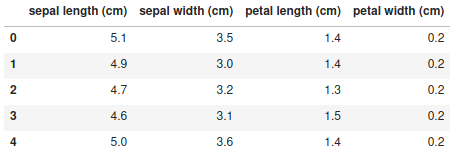
\includegraphics[width=0.4\textwidth]{cap04/dadosIris.png}
	\caption{DataFrame com os dados dos Atributos Preditores}
\end{figure}

O próximo passo é construir e treinar nosso modelo:
\begin{lstlisting}[]
clustering = KMeans(n_clusters=3, random_state=5).fit(X)
\end{lstlisting}

Normalmente para treinar um modelo passamos dois conjuntos de dados, porém o K-Means só recebe um único conjunto, exatamente por não realizar predições precisa apenas dos dados para separá-los em conjuntos. Mas como será que foi seu comportamento? Descobrimos isso comparando dois gráficos:
\begin{lstlisting}[]
cores = np.array(['green', 'red', 'blue'])
relabel = np.choose(clustering.labels_, [1, 0, 2]).astype(np.int64)
plt.figure(figsize = [15, 5])

plt.subplot(1, 4, 1)
plt.scatter(x=iris_df['petal length (cm)'], 
y=iris_df['petal width (cm)'], 
c=cores[iris.target], s=50)
plt.title('Real (Pétala)')

plt.subplot(1, 4, 2)
plt.scatter(x=iris_df['petal length (cm)'], 
y=iris_df['petal width (cm)'], 
c=cores[relabel], s=50)
plt.title('KMeans (Pétala)')

plt.subplot(1, 4, 3)
plt.scatter(x=iris_df['sepal length (cm)'], 
y=iris_df['sepal width (cm)'], 
c=cores[iris.target], s=50)
plt.title('Real (Sépala)')

plt.subplot(1, 4, 4)
plt.scatter(x=iris_df['sepal length (cm)'], 
y=iris_df['sepal width (cm)'], 
c=cores[relabel], s=50)
plt.title('KMeans (Sépala)')

plt.show()
\end{lstlisting}

Usamos os mesmos conjuntos de cores para cada espécie, obtemos quatro gráficos comparativos: 1º largura e altura da Pétala e a cor será mostrada com base em nosso atributo alvo (ou seja o valor real), 2º o que o modelo achou que seria o correto, 3º largura e altura da Sépala e o 4º novamente como o modelo separou. E obtemos como resultado:
\begin{figure}[H]
	\centering
	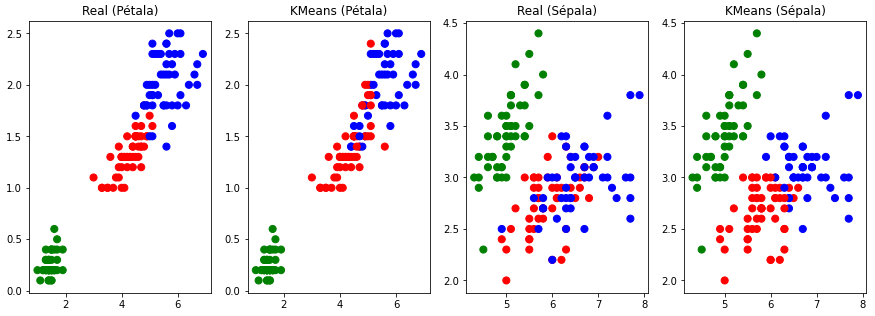
\includegraphics[width=0.8\textwidth]{cap04/comparativo.png}
	\caption{Comparativo entre o Real e o KMeans}
\end{figure}

Para pétala o \textbf{K-Means} quase acertou a posição de cada espécie, porém para Sépala aconteceram as maiores confusões, isso se deve ao fato do centroide. Para melhor avaliarmos nosso modelo precisamos de mais medidas: \textit{Precision} (precisão) é a medida de relevância do modelo, \textit{Recall} (revocação ou sensibilidade) se trata da medida de completude do modelo e \textit{F1 Score} se trata de uma média ponderada entre \textit{precision} e \textit{recall}. Podemos obtê-las da seguinte forma:
\begin{lstlisting}[]
metricas = classification_report(y, relabel)
print(metricas)
\end{lstlisting}

Obtemos como resultado:
\begin{figure}[H]
	\centering
	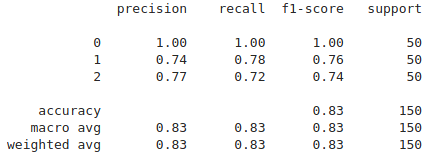
\includegraphics[width=0.6\textwidth]{cap04/relatorio.png}
	\caption{Relatório de Performance do K-Means}
\end{figure}

\textit{Precision} - É a razão entre as observações positivas previstas corretamente e o total de observações positivas previstas. Calculada com a fórmula: $TP \div (TP + FP)$.

\textit{Recall} - É a razão entre as observações positivas previstas corretamente e todas as observações da classe real. Calculada com a fórmula: $TP \div (TP + FN)$

\textit{F1 Score} - Essa pontuação leva em consideração tanto os falsos positivos quanto os negativos. Intuitivamente, não é tão fácil entender como precisão, mas F1 é geralmente mais útil que \textit{precision}, especialmente se estivermos com uma distribuição de classe desigual. $2 \times (recall \times precision) \div (recall + precision)$

\textit{Acurácia} funciona melhor se os falsos positivos e negativos tiverem um custo semelhante. Se o custo for muito diferente, é melhor olharmos essas métricas. 

\section{Clusterização Hierárquica}\index{Modelos Iniciais}
Este é um modelo alternativo ao particionamento de \textit{cluster} no conjunto de dados, pode ser aplicado para encontrar a distância entre cada ponto e seus vizinhos mais próximos e conectá-lo de forma ideal. Podemos mostrar o número de subgrupos com o auxílio de um Dendrograma\footnote{É um gráfico em formato de árvore que mostra visualmente os relacionamentos entre as observações.}. 

É útil pois não existe necessidade de especificar o número de \textit{clusters} (ou K) antes da análise e o dendrograma fornece uma representação visual desses. Vamos trazer para o conjunto de bibliotecas visto anteriormente mais três:
\begin{lstlisting}[]
from scipy.cluster.hierarchy import dendrogram, linkage
from sklearn.cluster import AgglomerativeClustering
from sklearn.metrics import accuracy_score
\end{lstlisting}

Para este exemplo vamos utilizar outra base que está contida no arquivo \textbf{mtcars.csv} (trazer essa para a subpasta \textbf{/base}). E carregamos os dados do seguinte modo:
\begin{lstlisting}[]
carros = pd.read_csv('bases/mtcars.csv')
carros.columns = ['name', 'mpg', 'cil', 'disp', 'hp', 'drat', 'wt', 'qsec', 'vs', 'am', 'gear', 'carb']
X = carros[['mpg', 'disp','hp', 'wt']].values
y = carros['am'].values
\end{lstlisting}

Essa base contém 32 modelos de carros com os seguintes atributos: Nome, autonomia em milhas por galão, número de cilindros, deslocamento (medida de poder do carro em polegada cúbica), cavalos de força, relação do eixo traseiro, peso (em libras), eficiência do gasto de combustível (por 1/4 milha), motor (0 = V-shaped, 1 = straight), câmbio (0 = automática, 1 = manual), total de marchas e carburadores. Porém para não trabalharmos com tantos atributos vamos usar somente: consumo de gasolina (mpg), deslocamento (disp), cavalos de força (hp) e peso (wt) e o nosso objetivo e descobrir se o carro possui um câmbio manual ou automático.

Podemos montar o dendrograma do seguinte modo: 
\begin{lstlisting}[]
z = linkage(X, 'ward')
dendrogram(z, truncate_mode='lastp', p=12, leaf_rotation=45, leaf_font_size=15, show_contracted=True)

plt.title('Dendograma')
plt.xlabel('Tamanho do Cluster')
plt.ylabel('Distancia')
plt.axhline(y=500)
plt.axhline(y=150)
plt.show()
\end{lstlisting}

Obtemos como resultado:
\begin{figure}[H]
	\centering
	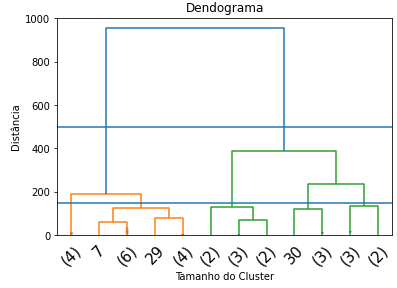
\includegraphics[width=0.6\textwidth]{cap04/dendrograma.png}
	\caption{Dendrograma dos tamanhos do Cluster}
\end{figure}

O dendrograma mostra como cada \textit{cluster} é composto e desenha um link em forma de U entre cada cluster e seus filhos. A parte superior indica uma mesclagem. Cada perna indica quais foram mesclados. O comprimento das pernas e do U representa a distância entre os filhos.

Para mesclar recursivamente o par de \textit{clusters} e aumentar minimamente a distância de ligação utilizamos a função AgglomerativeClustering(). Essa possui dois parâmetros básicos: \textit{affinity} e \textit{linkage}.

\textit{affinity}: métrica utilizada para calcular a ligação. Possui as seguintes opções:
\begin{itemize}[nolistsep]
	\item \textit{euclidean} - é o único que aceita o parâmetro \textit{linkage} como \textit{ward}. Refere-se a distância euclidiana que pode ser provada pela aplicação repetida do teorema de Pitágoras.
	\item \textit{l1} - critério de erro absoluto.
	\item \textit{l2} - critério de erros quadrados (lembramos do RSS).
	\item \textit{manhattan} - distância euclidiana ao quadrado.
	\item \textit{cosine} - também chamada de Similaridade do Cosseno. É a distância do cosseno entre duas variáveis.
	\item \textit{precomputed} - necessita de uma matriz de distância (em vez de similaridade) como entrada para o método de ajuste, pois X será considerado uma matriz.
\end{itemize}

\textit{linkage}: define qual o critério de ligação usar. Determina qual distância usar entre os conjuntos de observação. Possui as seguintes opções:
\begin{itemize}[nolistsep]
	\item \textit{ward} - minimiza a variação dos \textit{clusters} que estão sendo mesclados.
	\item \textit{average} - média das distâncias de cada observação dos conjuntos.
	\item \textit{complete} - distâncias máximas entre todas as observações dos dois conjuntos.
	\item \textit{single} - mínimo das distâncias entre todas as observações dos dois conjuntos.
\end{itemize}

Como escolher os parâmetros ideais? Fácil, testemos várias combinações e veremos qual possui uma melhor acurácia para os dados que estamos tratando:
\begin{lstlisting}[]
hclusters1 = AgglomerativeClustering(n_clusters=2, affinity='euclidean', linkage='ward').fit(X)
print('Método 1:', accuracy_score(y, hclusters1.labels_))

hclusters2 = AgglomerativeClustering(n_clusters=2, affinity='euclidean', linkage='complete').fit(X)
print('Método 2:', accuracy_score(y, hclusters2.labels_))

hclusters3 = AgglomerativeClustering(n_clusters=2, affinity='euclidean', linkage='average').fit(X)
print('Método 3:', accuracy_score(y, hclusters3.labels_))

hclusters4 = AgglomerativeClustering(n_clusters=2, affinity='manhattan', linkage='single').fit(X)
print('Método 4:', accuracy_score(y, hclusters4.labels_))

hclusters5 = AgglomerativeClustering(n_clusters=2, affinity='manhattan', linkage='complete').fit(X)
print('Método 5:', accuracy_score(y, hclusters5.labels_))

hclusters6 = AgglomerativeClustering(n_clusters=2, affinity='manhattan', linkage='average').fit(X)
print('Método 6:', accuracy_score(y, hclusters6.labels_))

hclusters7 = AgglomerativeClustering(n_clusters=2, affinity='cosine', linkage='single').fit(X)
print('Método 7:', accuracy_score(y, hclusters7.labels_))

hclusters8 = AgglomerativeClustering(n_clusters=2, affinity='cosine', linkage='complete').fit(X)
print('Método 8:', accuracy_score(y, hclusters8.labels_))

hclusters9 = AgglomerativeClustering(n_clusters=2, affinity='cosine', linkage='average').fit(X)
print('Método 9:', accuracy_score(y, hclusters9.labels_))
\end{lstlisting}

Obtemos como resultado: \\
{\ttfamily Método 1: 0.78125 \\
Método 2: 0.4375 \\
Método 3: 0.78125 \\
Método 4: 0.625 \\
Método 5: 0.71875 \\
Método 6: 0.71875 \\
Método 7: 0.3125 \\
Método 8: 0.28125 \\
Método 9: 0.1875}

Assim para esse caso \textit{Euclidian/Ward} ou \textit{Manhattan/Complete} são os que melhor responderam ao nosso conjunto de dados com uma acurácia de 78,12\%. Podemos inclusive tirar um relatório mais completo (como já vimos):
\begin{lstlisting}[]
print(classification_report(y, hclusters1.labels_))
\end{lstlisting}

Obtemos como resultado:
\begin{figure}[H]
	\centering
	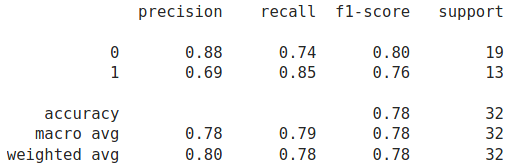
\includegraphics[width=0.6\textwidth]{cap04/relatorioHie.png}
	\caption{Relatório de Performance da Clusterização Hierárquica}
\end{figure}


Só que ficou uma pergunta no ar, esse método se comporta melhor que um modelo de clusterização preditivo como o KNN?

\subsection{Clusterização Hierárquica versus K-Nearest Neighbors}\index{Modelos Iniciais}
Para verificar como o KNN se comporta com os dados dos carros adicionamos mais quatro bibliotecas:
\begin{lstlisting}[]
from sklearn.neighbors import KNeighborsClassifier
from sklearn import preprocessing
from sklearn.model_selection import train_test_split
from sklearn.metrics import classification_report
\end{lstlisting}

Como já obtemos nossos dados, vamos apenas separá-los em bases de treino e teste:
\begin{lstlisting}[]
X = preprocessing.scale(X)
X_treino, X_teste, y_treino, y_teste = train_test_split(X, y, test_size=.20, random_state=17)
\end{lstlisting}

Porém devemos sempre lembrar que os modelos de clusterização trabalham melhor quando os dados estão em escala, assim acertamos os atributos preditores antes de realizar a separação de 80\% dos dados para treino e 20\% para teste.
\begin{lstlisting}[]
clf = KNeighborsClassifier()
clf.fit(X_treino, y_treino)
\end{lstlisting}

Treinamos nosso modelo e podemos avaliar o resultado:
\begin{lstlisting}[]
y_predito = clf.predict(X_teste)
print(classification_report(y_teste, y_predito))
\end{lstlisting}
	
Obtemos como resultado:
\begin{figure}[H]
	\centering
	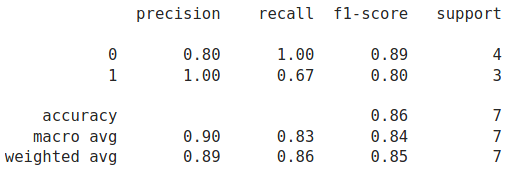
\includegraphics[width=0.5\textwidth]{cap04/relatorioKNN.png}
	\caption{Relatório de Performance do K-Nearest Neighbors}
\end{figure}

E na média percebemos que este se comporta melhor pois atinge resultados acima dos 80\%.

\section{Regressão Linear}\index{Modelos Iniciais}
A regressão linear tenta modelar o relacionamento entre dois atributos, através de ajustes sob uma equação linear dos dados observados. Um atributo é considerado \textbf{explicativo} e a outro \textbf{dependente}. Para simplificar um pouco, é uma técnica que utiliza valores de entrada para predizer os de saída (como por exemplo, prever o crescimento da população de um País) através da aplicação dos coeficientes (também chamados de peso) da equação linear. 

Comecemos com a importação das bibliotecas que necessitamos:
\begin{lstlisting}[]
import pandas as pd
import numpy as np
from matplotlib import pyplot as plt
from sklearn.linear_model import LinearRegression

%matplotlib inline
\end{lstlisting}

A classe \textit{Linear Model} da \textit{Scikit-Learn} o método \textit{LinearRegression} para realizar nosso trabalho. Baixar a base de dados \textbf{PopBrasil.csv} que contém as observações de Crescimento da População Brasileira.
\begin{lstlisting}[]
df = pd.read_csv('bases/PopBrasil.csv')
df.head()
\end{lstlisting}

Obtemos como resultado:
\begin{figure}[H]
	\centering
	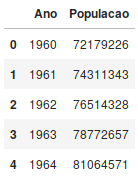
\includegraphics[width=0.15\textwidth]{cap04/basePop.png}
	\caption{Dados da População Brasileira}
\end{figure}

Devemos saber que o modelo trabalha com a relação entre atributos numéricos: explanatórios X e dependentes y. Utiliza somente esse tipo devido aos ajustes matemáticos que são realizados e os pesos criados conforme a função minimiza os erros. Nossas observações são bem simples: obtemos atributos numéricos, "Ano" e "População". Para entendermos o relacionamento entre os atributos, plotamos esses em um gráfico:
\begin{lstlisting}[]
plt.xlabel('Ano')
plt.ylabel('Quantidade da População')
plt.scatter(df.Ano, df.Populacao, color='red', marker='+')
\end{lstlisting}

Obtemos como resultado:
\begin{figure}[H]
	\centering
	\includegraphics[width=0.4\textwidth]{cap04/grafRelAnoPop.png}
	\caption{Dados da População Brasileira}
\end{figure}

E esta é a parte mais importante na execução desse modelo, a medida que alteramos o valor de "Ano" o valor de "População" também é afetado, ou seja, existe um relacionamento linear. Essa é a premissa básica para se usar este algoritmo, o relacionamento forte entre os atributos deve existir.

\subsection{Aplicar a Regressão Linear}\index{Modelos Iniciais}
Agora que obtemos nossos atributos conferidos, basta treinarmos nosso modelo e obtermos nossa previsão:
\begin{lstlisting}[]
reg = LinearRegression()
reg.fit(df[['Ano']], df.Populacao)
prev = reg.predict([[2020]])
print("Previsão 2020 é: %d" % prev)
\end{lstlisting}

E obtemos a predição da população brasileira para o ano de 2020, que é 221.322.254 de habitantes. Como a magia acontece? Pura matemática que é fornecida pela seguinte fórmula:
\begin{figure}[H]
	\centering
	\includegraphics[width=0.5\textwidth]{cap04/formulaRL.png}
	\caption{Base da Regressão Linear}
\end{figure}

\begin{note}[Para saber mais]{}
	Se deseja conhecer mais sobre o assunto, visite a página: \url{https://www.mathsisfun.com/algebra/linear-equations.html} aonde se obtém uma explicação mais completa.
\end{note}

E podemos reproduzir esse resultado pois o objeto treinado nos fornece tanto o valor do Gradiente (\textit{coef\_[0]}) quanto do Interceptador (\textit{intercept\_}). Então:
\begin{lstlisting}[]
m = reg.coef_[0]
b = reg.intercept_
prev2020 = m * 2020 + b
print("Previsão 2020 é: %d" % prev2020)
\end{lstlisting}

E obtemos exatamente o mesmo resultado. Podemos traçar a "Reta da Regressão Linear", pois o modelo consegue predizer os resultados de cada ano:
\begin{lstlisting}[]
plt.xlabel('Ano')
plt.ylabel('Quantidade da População')
plt.scatter(df.Ano, df.Populacao, color='red', marker='+')
plt.plot(df.Ano, reg.predict(df[['Ano']]), color='blue')
\end{lstlisting}

Obtemos como resultado:
\begin{figure}[H]
	\centering
	\includegraphics[width=0.5\textwidth]{cap04/grafRelAnoPopReta.png}
	\caption{Dados da População Brasileira com a Previsão}
\end{figure}

Vamos praticar nossos novos "poderes de futurólogo", junto a essa base encontramos outra chamada ExpecVida.csv, com ela, tente prever qual será a Expectativa de Vida do brasileiro no ano de 2020.

\subsection{Regressão Linear com mais de um Preditor}\index{Modelos Iniciais}
Vimos como usar o modelo de Regressão Linear, porém apenas a título de facilitação do entendimento, somente um atributo preditor. Mas o que acontece quando o alvo é influenciado por mais de um preditor? Vamos entender na prática como isso acontece.

Pensemos em um caso do Varejo, vamos utilizar um conjunto de observações chamado \textbf{marketSales.csv} que como o nome sugere, são compostos por transações de vendas. Sabemos que várias coisas influenciam a saída de um determinado produto, tais como, o grau de visibilidade, peso, se possui muita ou pouca quantidade de gordura, tamanho do mercado ou outros.

Começamos com a importação da bibliotecas necessárias:
\begin{lstlisting}[]
import pandas as pd
from sklearn.linear_model import LinearRegression
from sklearn.preprocessing import LabelEncoder
from sklearn.model_selection import train_test_split
from matplotlib import pyplot as plt

%matplotlib inline
\end{lstlisting}

E ler nossa base de dados:
\begin{lstlisting}[]
df = pd.read_csv('bases/marketSales.csv')
df.head()
\end{lstlisting}

Até o momento nada de novo, nosso problema começa ao repararmos nas observações:
\begin{figure}[H]
	\centering
	\includegraphics[width=0.5\textwidth]{cap04/dadosMarket.png}
	\caption{Observações sobre Vendas de Produtos}
\end{figure}

Sabemos que os modelos de regressão só trabalham com tipos numéricos, muito pior existe o caso de nulos entre algumas outras inconsistências  nessas 14.204 observações.

\subsection{Regressão Linear e Limpeza dos Dados}\index{Modelos Iniciais}
Sejamos francos, maior parte de trabalho do Cientista de Dados é arrumar os dados que sofridamente conseguiu para realizar o trabalho, então começaremos a compreender como uma parte disso funciona. Primeiro detalhe vamos tratar os atributos indesejáveis, nulos e que não contribuem em absolutamente em nada para o aumento/diminuição das vendas. Atributos como o código identificador do produto (\textit{Item\_Identifier}) e do mercado (\textit{Outlet\_Identifier}) - por esse motivo que o Cientista de Dados deve entender do negócio.

Ao verificarmos a função \textit{info()} descobrimos ainda que o atributo alvo (\textit{Item\_Outlet\_Sales}) que indica a quantidade de produtos vendidos possui dados nulos (ou seja, também não servem para previsão).
\begin{lstlisting}[]
df = df.drop(df[df['Item_Outlet_Sales'].isnull()].index)
df = df.drop(columns=['Item_Identifier', 'Outlet_Identifier'], axis=1)
\end{lstlisting}

Cuidado pois se aplicamos um corte seco como: {\ttfamily df.dropna(how='any',inplace=True)} obtemos somente 4.650 observações (devido a eliminação dos valores nulos contidos em outros atributos) - ou seja perdemos quase 10.000 observações. Lembrar que o tratamento dos nulos deve ser cirúrgico e criterioso. Ao aplicar o corte corretamente somente do atributo alvo ficamos com 8.523 observações. Além disso removemos os preditores que não serviam.

Nosso próximo problema com nulos é nos atributos: peso do item (\textit{Item\_Weight}) e tamanho da loja (\textit{Outlet\_Size}). Em um caso de dados real devemos procurar preencher esses valores solicitando a informação necessária aos responsáveis, porém para fins desse trabalho iremos remover essa colunas também.
\begin{lstlisting}[]
df = df.drop(columns=['Item_Weight', 'Outlet_Size'], axis=1)
\end{lstlisting}

Não obtemos mais a presença de nulos, mas ainda existem problemas, precisamos verificar os atributos não numéricos das observações, isto é: conteúdo de gordura (\textit{Item\_Fat\_Content}), tipo do item (\textit{Item\_Type}), localização da loja (\textit{Outlet\_Location\_Type}) e tipo da loja (\textit{Outlet\_Type}). Para isso:
\begin{lstlisting}[]
print("Gordura:", df['Item_Fat_Content'].unique())
print("Tipo:", df['Item_Type'].unique())
print("Loc. Loja:", df['Outlet_Location_Type'].unique())
print("Tipo Loja:", df['Outlet_Type'].unique())
\end{lstlisting}

O atributo \textit{Item\_Fat\_Content} possui uma faixa com os seguintes valores: '\textit{LF}', '\textit{Low Fat}', '\textit{Regular}', '\textit{low fat}' ou '\textit{reg}'. Obviamente só existem dois tipos: '\textit{Low Fat}' e '\textit{Regular}' os outros três são variações desses valores. Para corrigir isso e realizar sua conversão: 
\begin{lstlisting}[]
df['Item_Fat_Content'] = df['Item_Fat_Content'].map({'LF': 1, 'Low Fat': 1, 'low fat': 1, 'reg': 2, 'Regular': 2})
df['Item_Fat_Content'] = df['Item_Fat_Content'].astype(pd.Int64Dtype())
df['Outlet_Location_Type'] = df['Outlet_Location_Type'].map({'Tier 1': 1, 'Tier 2': 2, 'Tier 3': 3})
df['Outlet_Location_Type'] = df['Outlet_Location_Type'].astype(pd.Int64Dtype())
df['Outlet_Type'] = df['Outlet_Type'].map({'Supermarket Type1': 1, 'Supermarket Type2': 2, 'Supermarket Type3': 3, 'Grocery Store': 4})
df['Outlet_Type'] = df['Outlet_Type'].astype(pd.Int64Dtype())
\end{lstlisting}

Criamos um dicionário com as faixas, repetimos os mesmos valores para os tipos que são semelhantes e realizamos a troca dos elementos no \textit{DataFrame}. Aplicamos também a mesma prática para a localização e tipo da loja que possui poucos valores. Vamos agora com o caso de tipo do item que devemos trocá-lo para uma forma diferente (é ideal quando existem muitos valores diferentes).

Cada atributo tem um tipo determinado, por exemplo, \textit{float} aceita números com pontos decimais, \textit{int} numéricos inteiros, \textit{string} caracteres, além disso \textit{Python} trabalha com um tipo especial denominado \textit{category}. Corresponde a uma determinada faixa de valores. Converter tipo do item em atributo categórico:
\begin{lstlisting}[]
df['Item_Type'] = df.Item_Type.astype('category')
\end{lstlisting}

Uma vez realizado esse processo podemos "codificá-lo":
\begin{lstlisting}[]
le_Item_Type = LabelEncoder()
df['Item_Type'] = le_Item_Type.fit_transform(df['Item_Type'])
df.head()
\end{lstlisting}

Para cada valor categorizado é atribuído um valor numérico (ou seja o mesmo trabalho que tivemos para o mapa). Usamos as funções \textit{info()} e \textit{describe()} e podemos partir para a próxima etapa sem quaisquer problemas com os dados, pois agora são todos numéricos e não possuem qualquer valor nulo.

\subsection{Separação e treino}\index{Modelos Iniciais}
Separar em treino e teste (para avaliarmos nosso modelo) e remover o atributo alvo:
\begin{lstlisting}[]
target = df['Item_Outlet_Sales']
df = df.drop(columns=['Item_Outlet_Sales'], axis=1)
X_train, X_test, y_train, y_test = train_test_split(df, target, test_size = .2)
print('Amostra de Treino:', X_train.shape)
print('Amostra de Teste:', X_test.shape)
\end{lstlisting}

Usamos um valor de 20\% para nosso teste e obtemos: 6.818 observações para treino e 1.705 de teste. Treinamos nosso modelo e verificamos seu resultado:
\begin{lstlisting}[]
clf = LinearRegression()
clf.fit(X_train, y_train)
print('Acurácia: ', clf.score(X_test, y_test))
\end{lstlisting}

E obtemos uma acurácia aproximada de 42\% e qual o motivo dessa discrepância tão grande? Simples, estamos cada vez mais perto da realidade e podemos verificar que realizar previsões com altos scores e poucas ações não existe. Pois se fosse assim: Corramos para treinar um modelo que nos dará os seis números da MegaSena. Ou ao menos nos dizer quando vai chover corretamente com muito pouco trabalho. Por fim podemos ver como os dados estão bem discrepantes em relação ao que foi predito e o real:
\begin{lstlisting}[]
y_pred = model.predict(X_test)
plt.plot(y_test, y_test)
plt.scatter(y_test, y_pred, c = 'red', marker='+')
plt.ylabel('Real')
plt.xlabel('Predito')
plt.show()
\end{lstlisting}

Obtemos como resultado:
\begin{figure}[H]
	\centering
	\includegraphics[width=0.5\textwidth]{cap04/regressaoFinal.png}
	\caption{Regressão Linear aplicada a vários atributos}
\end{figure}

Em vermelho são a relação entre o valor real e o que foi predito, a linha azul mostra a Reta da Regressão. Verificamos a presença de um ponto bem isolado? Pode ser um \textit{outlier}? Exatamente por esse motivo que passamos um bom tempo em EDA.

\section{Árvore de Decisão}\index{Modelos Iniciais}
Se existe uma unanimidade entre os modelos que todo o Cientista de Dados conhece \textit{Decision Tree} seria provavelmente o grande campeão (ou estaria entre os primeiros colocados), é um modelo com base em perguntas e respostas. Vamos começar com a importação das nossas bibliotecas básicas:
\begin{lstlisting}[]
import pandas as pd
import numpy as np
from sklearn.preprocessing import LabelEncoder
from sklearn import tree
\end{lstlisting}

Além da Pandas e NumPy, que serão básicas para todos os modelos que vemos, necessitamos também da \textit{LabelEncoder} que responde as manipulações no DataFrame e do objeto tree por conter a classe para executar o algorítimo. Próximo passo é buscarmos os nossos dados:
\begin{lstlisting}[]
df = pd.read_csv('bases/salaries.csv')
df.head()
\end{lstlisting}

Essa base de salários é composta por 3 empresas: Google, Facebook e ABC Pharma. Temos ainda Cargo, Grau de Ensino e Salário (Anual). E chegamos na parte essencial por adotar esse modelo: \textbf{O que desejamos responder?}, exatamente isso o modelo responde a uma pergunta que deve ser formulada de forma binária, ou seja que tal na empresa X, com um cargo Y e curso Z conseguimos ganhar um salário maior que 100 mil anuais?

Precisamos preparar nossa base de dados e adicionar uma resposta a nossa pergunta, assim criamos a variável \textbf{desejo}:
\begin{lstlisting}[]
desejo = pd.Series(np.where(df['salary']>=100000, 1, 0))
print(desejo)
\end{lstlisting}

Observamos que desejo possui somente os valores 0 e 1 que indica falso ou verdadeiro para cada um dos itens da nossa tabela original. Por exemplo: trabalhar na Google, com um curso de Bacharel no cargo Executivo de Vendas não fará ganhar um salário de 100 mil anuais, mas no cargo Gerente de Negócios sim.

Para criarmos nossa Árvore de Decisão, precisamos que todos os campos (que participarão de sua composição) sejam variáveis numéricas categóricas, sua formação se dará da seguinte forma:
\begin{figure}[H]
	\centering
	\includegraphics[width=0.5\textwidth]{cap04/arvore}
	\caption{Estrutura da Árvore Montada}
\end{figure}

A função da biblioteca LabelEncoder é fazer exatamente isso, ou seja, transformar uma variável caractere, criar uma categoria e atribuir uma valor para ela, então:
\begin{lstlisting}[]
le_company = LabelEncoder()
le_job = LabelEncoder()
le_degree = LabelEncoder()

df['company_n'] = le_company.fit_transform(df['company'])
df['job_n'] = le_company.fit_transform(df['job'])
df['degree_n'] = le_company.fit_transform(df['degree'])
df.head()
\end{lstlisting}

Criamos 3 novas séries e adicionamos ao nosso DataFrame original, vemos que foi atribuído um valor numérico para cada categoria, por exemplo Google é 2, Business Manager (Gerente de Negócios) é 0. Dessa forma que o algorítimo monta nossa árvore, a partir dessas três variáveis. Porém precisamos de um \textit{DataFrame} composto somente por elas:
\begin{lstlisting}[]
entradas = df.drop(['company','job','degree','salary'], axis='columns')
entradas.head()
\end{lstlisting}

De um modo mais simples, criamos um novo \textit{DataFrame} (entradas) sem as variáveis descritivas (Empresa, Cargo e Grau de Ensino) e a numérica (Salário). Tudo está pronto, com esses dois novos objetos (\textbf{desejo} e \textbf{entradas}) podemos treinar nosso algorítimo:
\begin{lstlisting}[]
model = tree.DecisionTreeClassifier()
model.fit(entradas, desejo)
\end{lstlisting}

E podemos realizar nossas perguntas, por exemplo, alguém da \textbf{Google} (2) que trabalha no cargo \textbf{Executivo de Vendas} (2) e fez \textbf{Mestrado} (1) recebe um salário maior que 100 mil anuais?
\begin{lstlisting}[]
model.predict([[2, 2, 1]])
\end{lstlisting}

E obtemos como resposta o valor \textbf{0} indicando que não. Este é um dos principais modelos utilizados em Ciência de Dados tornou-se a porta de entrada para muitos outros. Podemos nos enganar com o pensamento que bastaria dar uma olhada nos dados para respondermos a pergunta, em uma base pequena realmente isso pode até ser viável, porém em uma base com muitos dados seria impraticável.

\subsection{Critérios Gini e Entropia}\index{Modelos Iniciais}
Uma árvore de decisão se enquadra nos Algoritmos para Aprendizado de Máquina supervisionados e pode ser usada tanto para classificação quanto regressão - embora principalmente para o primeiro tipo. Como vimos este modelo obtém uma instância, atravessa uma árvore e compara recursos importantes com uma determinada declaração condicional. Se ele desce para o ramo filho esquerdo ou direito depende do resultado. Normalmente, os recursos mais importantes estão próximos a raiz.

Existem dois critérios que são comumente passados, são consideradas métricas padrão para calcular "impureza" ou "nível de informação". Orientam a divisão de um nó na árvore de decisão apenas com base nas informações existentes nesse nó. São calculados conforme as seguintes fórmulas:
\begin{itemize}
	\item Gini: $1 - \sum_{j=1}^{c} (p_{j})^{2}$
	\item Entropy: $-\sum_{j=1}^{c} p_{j} \times log(p_{j})$
\end{itemize}

\textbf{Gini} é a probabilidade de uma amostra aleatória ser classificada incorretamente se escolhermos aleatoriamente um \textit{label} de acordo com a distribuição em um ramo. \textbf{Entropia} é uma medida de informação (ou melhor, a falta dela). Ao calcular o ganho de informação sobre uma divisão. Qual é a diferença em entropias. Isso mede como se reduz a incerteza sobre um \textit{label}.

Vamos começar um outro projeto, porém veremos algo bem diferente, não iremos nos preocupar em explanar os dados que exploraremos. Vamos iniciar pelas bibliotecas:
\begin{lstlisting}[]
import pandas as pd
from sklearn.model_selection import train_test_split
from sklearn.tree import DecisionTreeClassifier
from sklearn.metrics import accuracy_score
from sklearn.metrics import classification_report
from sklearn.metrics import confusion_matrix
\end{lstlisting}

A grande diferença esta aqui: criamos um conjunto de funções para realizar todo o trabalho de leitura, separação e execução do modelo. Recomendo esse método quando for criar seus projetos, pois simplifica muito a manutenção dos mesmos:
\begin{lstlisting}[]
def obterDados(base):
  balance_data = pd.read_csv(base, sep = ',', header = None)
  print('Tamanho:', balance_data.shape)
  print(balance_data.head())
  return balance_data

def separarDados(dados):
  x = dados.values[:,1:5]
  y = dados.values[:,0]
  x_train, x_test, y_train, y_test = train_test_split(x, y, test_size = 0.3, random_state = 100)
  return x, y, x_train, x_test, y_train, y_test

def treinar(x_train, y_train, criterio):
  clf = DecisionTreeClassifier(criterion = criterio, random_state = 100, max_depth = 3, min_samples_leaf = 5)
  clf.fit(x_train,y_train)
  return clf

def predizer(x_test, clf):
  y_pred = clf.predict(x_test)
  print(f"Valores Preditos: {y_pred}")
  return y_pred

def acuracia(y_test, y_pred):
  print("Acurácia:", accuracy_score(y_test, y_pred, average='weighted', zero_division=1) * 100)
  print(confusion_matrix(y_test, y_pred))
  print(classification_report(y_test, y_pred))
\end{lstlisting}

O \textit{obterDados()} é responsável por ler e devolver as informações da nossa base de dados, \textit{separarDados()} por dividir corretamente nossa base em treino e teste, \textit{treinar()} realiza o treinamento da base conforme determinado critério, \textit{predizer()} obtém as predições com base na massa de teste em conjunto com o classificador e \textit{acuracia()} verifica os resultados obtidos.

Com algumas mudanças podemos adaptar esses métodos e começar a pensar em criar uma biblioteca de modo a facilitar nossos projetos futuros. Veja como é mais simples com seu uso.

Para ler os dados:
\begin{lstlisting}[]
data = obterDados('bases/balance-scale.data')
\end{lstlisting}

Para separar os dados:
\begin{lstlisting}[]
x, y, x_train, x_test, y_train, y_test = separarDados(data)
\end{lstlisting}

Treinar com o critério \textbf{Gini}:
\begin{lstlisting}[]
clf = treinar(x_train, y_train, 'gini')
y_pred_gini=prediction(x_test, clf)
\end{lstlisting}

Obter o resultado:
\begin{lstlisting}[]
cal_accuracy(y_test, y_pred_gini)
\end{lstlisting}

E obtemos como resultado:
\begin{figure}[H]
	\centering
	\includegraphics[width=0.45\textwidth]{cap04/relatorioGini}
	\caption{Resultado para o Critério Gini}
\end{figure}

Treinar com o critério \textbf{Entropia}:
\begin{lstlisting}[]
clf = treinar(x_train, y_train, 'entropy')
y_pred_entr = prediction(x_test, clf)
\end{lstlisting}

Obter o resultado:
\begin{lstlisting}[]
acuracia(y_test, y_pred_entr)
\end{lstlisting}

E obtemos como resultado:
\begin{figure}[H]
	\centering
	\includegraphics[width=0.45\textwidth]{cap04/relatorioEntropia}
	\caption{Resultado para o Critério Entropia}
\end{figure}

E observamos que neste caso, Gini possui uma melhor resposta aos dados.

\section{Floresta Aleatória}\index{Modelos Iniciais}
\textit{Random Forest} (por caridade \textit{Florest} não existe na língua inglesa) é um modelo supervisionado que pode ser considerado como um aprimoramento da Árvore de Decisão, vamos recapitular seu funcionamento.

Através de um conjunto definido de regras, um novo valor passará por uma série de perguntas, os chamados ramos da árvore, para prevermos em qual melhor resposta se encaixa. Agora vamos pensar que podemos separar os dados em várias partes definidas aleatoriamente e usarmos uma árvore para cada uma dessas partes e para tomarmos uma decisão apenas computamos qual foi a resposta mais votada?
\begin{figure}[H]
	\centering
	\includegraphics[width=0.65\textwidth]{cap04/florestaFunciona}
	\caption{Funcionamento da Floresta Aleatória}
\end{figure}

E esse é o conceito da \textbf{Floresta Aleatória}, para aprendermos como é esse modelo na prática. Começamos com a importação das bibliotecas:
\begin{lstlisting}[]
import pandas as pd
from sklearn.model_selection import train_test_split
from sklearn.datasets import load_digits
from sklearn.ensemble import RandomForestClassifier
from sklearn.metrics import confusion_matrix
import matplotlib.pyplot as plt
import seaborn as sn

plt.figure(figsize=(10,7))
%matplotlib inline
\end{lstlisting}

A única aquisição nova é o método \textit{RandomForestClassifier} que vem da ensemble contida na biblioteca \textit{Scikit-learn}. Como fonte de dados usamos os dados de \textit{load\_digits} (isso mesmo, finalmente vamos trabalhar com imagens). Lemos nossos dados:
\begin{lstlisting}[]
digits = load_digits()
\end{lstlisting}

E verificamos um determinado dígito, por exemplo o 8:
\begin{lstlisting}[]
plt.matshow(digits.images[8])
plt.show()
\end{lstlisting}

E obtemos como resultado:
\begin{figure}[H]
	\centering
	\includegraphics[width=0.3\textwidth]{cap04/imagemFormada}
	\caption{Número 8 da load\_digits}
\end{figure}

Uma imagem é formada por vários pontos que denominamos de pixels, cada um desses possuem valor em uma escala de cores, no caso dessa base obtemos 64 colunas identificando cada um desses pontos. Vamos criar um DataFrame com esses dados:
\begin{lstlisting}[]
df = pd.DataFrame(digits.data)
df.head()
\end{lstlisting}

E obtemos como resultado:
\begin{figure}[H]
	\centering
	\includegraphics[width=0.7\textwidth]{cap04/dadosDaImagem}
	\caption{Dados das Imagens}
\end{figure}

O problema é que não existe como coluna o resultado e precisamos colocá-lo, esse valor está no elemento target (não pense que existem apenas 9 imagens, são 1.997):
\begin{lstlisting}[]
df['valor'] = digits.target
\end{lstlisting}

Separamos nossos dados na massa de treino e teste (20\% do total):
\begin{lstlisting}[]
X_train, X_test, y_train, y_test = train_test_split(df.drop(['valor'], axis='columns'), df['valor'], test_size = .2)
print(len(X_train), len(X_test))
\end{lstlisting}

E treinamos nosso modelo:
\begin{lstlisting}[]
clf = RandomForestClassifier()
clf.fit(X_train, y_train)
\end{lstlisting}

Observamos no resultado o parâmetro "n\_estimators=100", isso significa que são 100 árvores na nossa floresta, podemos aumentar ou diminuir (sem pensar em desmatamento) o número dessas árvores e observar se conseguimos aumentar nosso resultado. Verificamos a acurácia:
\begin{lstlisting}[]
clf.score(X_test, y_test)
\end{lstlisting}

E obtemos significativos 98\%, ou seja, nosso modelo erra apenas 2\% das vezes, o que pode ser visto na Matriz de Confusão :
\begin{lstlisting}[]
y_predicted = clf.predict(X_test)
cm = confusion_matrix(y_test, y_predicted)
sn.heatmap(cm, annot=True, cmap=plt.cm.Blues)
plt.xlabel('Predito')
plt.ylabel('Verdadeiro')
plt.show()
\end{lstlisting}

Obtemos como resultado:
\begin{figure}[H]
	\centering
	\includegraphics[width=0.7\textwidth]{cap04/matriz2}
	\caption{Matriz de Confusão no Seaborn}
\end{figure}

\clearpage

% Modelos Preditivos: 
% %------------------------------------------------------------------------------------
%	CHAPTER 5
%------------------------------------------------------------------------------------
\chapterimage{headConceito.png}
\chapter{Modelos Preditivos}

\begin{remark}
O que sabemos é uma gota; o que ignoramos é um oceano. (Isaac Newton - Astrônomo) 
\end{remark}

\section{Naïve Bayes}\index{Modelos Preditivos}
As pessoas pensam que o Cientista de Dados possui Contatos do Além e podem prever números da MegaSena ou um Desastre de Avião quando se fala em "Predição", sinto não somos charlatões, podemos pegar todos resultados da MegaSena e demonstrar com base em modelos quais os números que mais ou menos saíram, ou analisar os dados físicos de um avião, cruzar isso com todos os voos que já se acidentaram e tentar traçar uma característica. Em ambos os casos não espere certeza, existe o que chamamos: "Probabilidade de Acontecer".

Naïve Bayes é o tipo de algorítimo que dá medo em muito Cientista novato, talvez seja porque aparenta ser o mais matemático possível, sua descrição precisa seria "classificador probabilístico baseado no Teorema de Bayes, o qual foi criado por Thomas Bayes (1701 - 1761)". Para não assustar ninguém, devemos saber que trata-se de um Algorítimo Supervisionado destinado a probabilidades. Resumidamente: Qual a probabilidade de um evento A ocorrer dado que um evento B ocorreu? Qual a probabilidade de um e-mail ser spam dado que chegou um e-mail? Ativamos nosso JupyterLab personalizado que criamos com o Docker e na primeira célula importamos as bibliotecas necessárias:
\begin{lstlisting}[]
import numpy as np
import pandas as pd

from sklearn.naive_bayes import MultinomialNB
from sklearn.naive_bayes import BernoulliNB
from sklearn.naive_bayes import GaussianNB
from sklearn.model_selection import train_test_split
from sklearn.metrics import accuracy_score
\end{lstlisting}

Além das bibliotecas tradicionais como Pandas e NumPy para manipulação dos dados, temos todo o pacote da Naive\_Bayes para os três tipos do modelo:
\begin{itemize}[nolistsep]
	\item Multinominal - realizar predições quando as variáveis (categóricas ou contínuas) descrevem contas discretas de frequência.
	\item Bernoulli - realizar predições para variáveis binárias.
	\item Gaussiano - realizar predições para campos de distribuição normal.
\end{itemize}
	
Por fim e não menos importante a biblioteca para separação das amostras de treino e testes além da biblioteca para medir a acurácia dos nossos modelos e ver a que melhor atende. Agora vamos baixar o arquivo \textbf{spambase.data} acessar nossos dados:
\begin{lstlisting}[]
dataset = np.loadtxt('bases/spambase.data', delimiter=',')
print(dataset[0])
\end{lstlisting}

Nessa base em cada observação existem 48 variáveis explanatórias com valores numéricos classificados e a 49ª é nossa variável resposta que indica se esse e-mail é ou não um Spam. Assim precisamos separar nossa massa de treino e teste:
\begin{lstlisting}[]
X = dataset[:, 0:48]
y = dataset[:, -1]
X_train, X_test, y_train, y_test = train_test_split(X, y, test_size = .33, random_state = 17)
\end{lstlisting}

Nossa amostra para teste será formada por 33\% do total, o que nos permite avaliar muito bem a performance de cada um dos tipos do modelo.

\subsection{Tipo Multinominal}\index{Modelos Preditivos}
Basicamente a codificação não difere muito entre usar um tipo ou outro:
\begin{lstlisting}[]
MultiNB = MultinomialNB() # 1
MultiNB.fit(X_train, y_train) # 2
print(MultiNB)
y_expect = y_test # 3
y_pred = MultiNB.predict(X_test) # 4
print(accuracy_score(y_expect, y_pred))
\end{lstlisting}

Quatro passos básicos para cada um deles, (1) criamos um objeto do tipo selecionado, (2) executamos nossa massa de treino, (3) guardamos nosso resultado de teste, realizamos a predição com o uso da massa de teste (4) como resultado teremos a acurácia do modelo em acertar. Que neste caso gerou um valor de 0.8736010533245556, que significa em 87\% das vezes o modelo foi eficaz.

\subsection{Tipo Bernoulli}\index{Modelos Preditivos}
Nosso próximo teste será feito para o tipo Bernoulli:
\begin{lstlisting}[]
BernNB = BernoulliNB(binarize = 0.0)
BernNB.fit(X_train, y_train)
print(BernNB)
y_expect = y_test
y_pred = BernNB.predict(X_test)
print(accuracy_score(y_expect, y_pred))
\end{lstlisting}

Comparando os códigos veremos basicamente as mesmas coisas com a diferença do tipo selecionado e um parâmetro chamado "Binarização", esse é um tipo de modelo que "ama" variáveis binárias quanto mais tiver nos dados melhor, é um parâmetro de valor numérico flutuante (por padrão o valor é 0,0) e como resultado temos um valor de 0.8130348913759052, ou seja, 81\% e se pararmos para pensar resultado pior que o tipo anterior, pois bem façamos uma mudança e troquemos o parâmetro de entrada:
\begin{lstlisting}[]
BernNB = BernoulliNB(binarize = 0.1)
\end{lstlisting}

E com essa mudança nosso resultado muda para o valor 0.8953258722843976. Não pense erradamente que agora virou festa e quanto mais aumentarmos o valor do parâmetro melhor será nossa acurácia. Realize testes e constate que pode obter resultados piores. Então tudo é uma questão de ajustarmos os parafusos (e esse é o real trabalho do Cientista de Dados em relação aos modelos).

\subsection{Tipo Gaussiano}\index{Modelos Preditivos}
E novamente voltamos ao básico:
\begin{lstlisting}[]
GausNB = GaussianNB()
GausNB.fit(X_train, y_train)
print(GausNB)
y_expect = y_test
y_pred = GausNB.predict(X_test)
print(accuracy_score(y_expect, y_pred))
\end{lstlisting}

Mas como resultado temos uma acurácia baixa de 0.8130348913759052, se for comparada obviamente aos outros resultados.

\subsection{Conclusão}\index{Modelos Preditivos}
Então constatamos que para essa massa de dados o Naïve Bayes tipo Bernoulli com o parâmetro definido para o valor 0,1 possui uma melhor acurácia de 89\%. Agora é sentar e realizar testes de como outra massa de dados se comporta.

\section{Apriori}\index{Modelos Preditivos}
Quando vamos no supermercado, normalmente encontramos o sal grosso perto da carne de churrasco (ou do carvão), ou quando uma loja começa a indicar ofertas de coisas que realmente precisamos? Isso não é sorte (nem Magia Negra) é chamado de ARM ou "Mineração por Regras de Associação" e esse próximo modelo faz exatamente isso.

O ARM (Associate Rule Mining) é uma das técnicas importantes em ciência de dados. No ARM, a frequência de padrões e associações no conjunto de dados é identificada entre os conjuntos de itens usados para prever o próximo item relevante no conjunto. Principalmente nas decisões em negócios de acordo com os gostos dos clientes. Porém precisamos instalar sua biblioteca com o comando:
\begin{lstlisting}[]
!pip install apyori
\end{lstlisting}

Apriori é um algoritmo de aprendizagem não supervisionado que é utilizado na modalidade ARM. Sua função é procurar por uma série de conjuntos frequentes em itens de dados e se baseia em associações e correlações entre esses conjuntos de itens. É o algoritmo por trás do "Você também pode gostar de..." que costumamos encontrar nas plataformas de recomendação.

Tudo pronto e podemos importar as bibliotecas necessárias:
\begin{lstlisting}[]
import pandas as pd
from apyori import apriori
\end{lstlisting}

Diferente dos alguns outros modelos, esse algorítimo não se encontra sobre a Scikit-Learn mas sobre a biblioteca apyori. E estamos usando a Pandas somente para facilitar o trabalho de ler um arquivo CSV e depois retornar os dados de forma fácil. Baixamos a base de dados \textbf{store\_data.csv} e a lemos com o comando:
\begin{lstlisting}[]
store_data = pd.read_csv('bases/store_data.csv', header=None)
store_data.head()
\end{lstlisting}

O detalhe aqui é que usaremos o cabeçalho como uma linha de dados válido, pois o modelo usa para criar as associações. A biblioteca Apriori exige que nosso conjunto de dados esteja na forma de uma lista de listas, onde todo o conjunto de dados é uma grande lista e cada transação no conjunto de dados é uma lista interna da grande lista externa.
\begin{lstlisting}[]
records = []
for i in range(0, 7501):
records.append([str(store_data.values[i,j]) for j in range(0, 20)])
\end{lstlisting}

O primeiro valor para o laço de repetição (7501) vem do número de linhas que contém nosso modelo enquanto que o seguindo valor do laço (20) é o número de colunas.

Assim temos os dados prontos para trabalharmos. Um detalhe importante, este modelo se utiliza de três variáveis:
\begin{itemize}[nolistsep]
	\item Suporte (support): O suporte do item I é definido como a razão entre o número de transações que contêm o item I pelo número total de transações.
	\item Confiança (confidence): Isso é medido pela proporção de transações com o item I1, nas quais o item I2 também aparece. A confiança entre dois itens I1 e I2, em uma transação, é definida como o número total de transações contendo os itens I1 e I2 dividido pelo número total de transações contendo I1.
	\item Lift: uma tradução para a palavra seria "Aumento", porém esta é a razão entre a confiança e o suporte.
\end{itemize}

E assim criamos nossas listas de regras com base nos valores das 3 variáveis:

\begin{lstlisting}[]
regras = list(apriori(records, min_support=0.0045, min_confidence=0.2, min_lift=3, min_length=2))
\end{lstlisting}

Temos como resultado 48 regras, apenas para facilitar a leitura vamos usar a seguinte codificação para visualizar os resultados:
\begin{lstlisting}[]
for item in regras:
items = [x for x in item[0]]
print("Regra: " + items[0] + " -> " + items[1])
print("Suporte: " + str(item[1]))
print("Confiança: " + str(item[2][0][2]))
print("Lift: " + str(item[2][0][3]))
print("=====================================")
\end{lstlisting}

Para entendermos como funciona, vamos ver a primeira regra:
\begin{figure}[H]
	\centering
	\includegraphics[width=0.7\textwidth]{cap05/apriori1}
	\caption{Primeira regra obtida}
\end{figure}

Entre o "Frango" e o "Creme Light". O valor de suporte é 0,0045 (este número é calculado dividindo o número de transações que contêm o primeiro produto dividido pelo número total de transações). A confiança de 0,2905 significa que de todas as transações que contêm "Creme Light", 29,05\% também foi comprado "Frango". \textit{Lift} mostra que o "Creme Light" tem 4,84 vezes mais chances de ser comprado pelos clientes que compram "Frango", em comparação com a probabilidade de venda do "Creme Light".

Para fixarmos vejamos a próxima regra:
\begin{figure}[H]
	\centering
	\includegraphics[width=0.7\textwidth]{cap05/apriori2}
	\caption{Segunda regra obtida}
\end{figure}

Entre o "Molho de Creme de Cogumelos" e o "Escalope". O suporte é de 0,0057. A confiança de 0,3006 significa que de todas as transações que contêm o "Molho de Creme de Cogumelos" 30,06\% também contêm "Escalope". \textit{Lift} mostra que o "Escalope" tem 3,79 mais chances de ser comprado pelos clientes que compram o "Molho de Creme de Cogumelos", em comparação com a probabilidade de venda do "Escalope".

Pronto, agora já podemos ler todas as outras 46 regras criadas entre os produtos e aumentar as vendas do nosso negócio.

\section{SVM}\index{Modelos Preditivos}
\textit{Support Vector Machine} é um algorítimo supervisionado capaz de classificar, regredir e também encontrar outliers. Para entendê-lo vamos considerar a seguinte figura:
\begin{figure}[H]
	\centering
	\includegraphics[width=0.6\textwidth]{cap05/svm1}
	\caption{Comparação Muffin e Cupcake}
\end{figure}

Devemos nos perguntar aonde poderíamos colocarmos uma reta que separaria os dois grupos da melhor forma possível? Compreendendo isso matamos esse algorítimo. A nossa base será formada por percentuais com várias receitas de Muffin e Cupcake.

A função que daremos ao algorítimo será de identificar se trata de um ou outro. Vamos começar com a importação das bibliotecas necessárias:
\begin{lstlisting}[]
import pandas as pd
import numpy as np
from sklearn import svm
from sklearn import datasets
from sklearn.metrics import confusion_matrix
import matplotlib.pyplot as plt
import seaborn as sns; sns.set(font_scale=1.2)

%matplotlib inline
\end{lstlisting}

O algorítimo da SVM está na Scikit-Learn, porém precisamos entender que existem 3 classes distintas para se trabalhar com Classificação: \textbf{SVC}, \textbf{NuSVC} e \textbf{LinearSVC}. SVC e NuSVC são métodos semelhantes, mas possuem alguns parâmetros com algumas pequenas diferenças bem como formulações matemáticas. Por outro lado, o LinearSVC é outra implementação do Modelo para o caso de um kernel linear. Trabalharemos aqui com a SVC ou \textit{C-Support Vector Classification}.

Próximo trabalho é baixar a base \textbf{muffins\_cupcakes.csv} ler:
\begin{lstlisting}[]
recipes = pd.read_csv('bases/muffins_cupcakes.csv')
recipes.head()
\end{lstlisting}

Basicamente essa base contém as proporções dos seguintes ingredientes: Farinha (\textit{Flour}), Leite (\textit{Milk}), Açúcar (\textit{Sugar}), Manteiga (\textit{Butter}), Ovo (\textit{Egg}), Fermento (\textit{Baking Powder}), Essência de Baunilha (\textit{Vanilla}) e Sal (\textit{Salt}). Vamos separar Açúcar e Manteiga para treinar nosso modelo:
\begin{lstlisting}[]
ingrediente = recipes[['Sugar', 'Butter']].values
tipo = np.where(recipes['Type']=='Muffin', 0, 1)
\end{lstlisting}

E como é um modelo supervisionado, precisamos também indicar do que se trata a receita. Treinamos nosso modelo:
\begin{lstlisting}[]
model = svm.SVC(kernel='linear', decision_function_shape=None)
model.fit(ingrediente, tipo)
\end{lstlisting}

Uma vez feito isso, vamos criar dois pontos para definir uma linha (apenas para mostrar) como nossos dados são separados:
\begin{lstlisting}[]
w = model.coef_[0]
a = -w[0] / w[1]
xx = np.linspace(5, 30)
yy = a * xx - (model.intercept_[0]) / w[1]
\end{lstlisting}

Agora basta colocarmos tudo em um gráfico:
\begin{lstlisting}[]
sns.lmplot('Sugar', 'Butter', data=recipes, hue='Type', palette='Set1', fit_reg=False, scatter_kws={"s": 70});
plt.plot(xx, yy, linewidth=2, color='black');
\end{lstlisting}

E obtemos o seguinte resultado:
\begin{figure}[H]
	\centering
	\includegraphics[width=0.6\textwidth]{cap05/svm2}
	\caption{Comparação Muffin e Cupcake}
\end{figure}

Mas como essa linha é encontrada? Isso é feito com base em "margens". Criamos mais 2 linhas para entendermos o processo:
\begin{lstlisting}[]
b = model.support_vectors_[0]
yy_down = a * xx + (b[1] - a * b[0])
b = model.support_vectors_[-1]
yy_up = a * xx + (b[1] - a * b[0])
\end{lstlisting}

E ao colocar novamente tudo em um gráfico:
\begin{lstlisting}[]
sns.lmplot('Sugar', 'Butter', data=recipes, hue='Type', palette='Set1', fit_reg=False, scatter_kws={"s": 70})
plt.plot(xx, yy, linewidth=2, color='black')
plt.plot(xx, yy_down, 'k--')
plt.plot(xx, yy_up, 'k--')
plt.scatter(model.support_vectors_[:, 0], model.support_vectors_[:, 1], s=80, facecolors='none');
\end{lstlisting}

E obtemos o seguinte resultado:
\begin{figure}[H]
	\centering
	\includegraphics[width=0.6\textwidth]{cap05/svm3}
	\caption{Comparação Muffin e Cupcake}
\end{figure}

E é exatamente a partir da melhor "margem" que a linha é criada. O mais interessante que esse é um algorítimo de previsão, então vamos criar um pequeno método:
\begin{lstlisting}[]
def muffin_ou_cupcake(sugar, butter):
  if (model.predict([[sugar, butter]])) == 0:
    print('Isto é uma receita de Muffin')
  else:
    print('Isto é uma receita de Cupcake')
\end{lstlisting}

E podemos fazer algumas verificações:
\begin{lstlisting}[]
muffin_ou_cupcake(20, 10)
\end{lstlisting}

E isso nos diz que provavelmente trata-se de um Muffin!

\subsection{Retorno a Íris}\index{Modelos Preditivos}

Vamos retornar as nossas flores para entendermos mais algumas coisas sobre esse modelo:
\begin{lstlisting}[]
iris = datasets.load_iris()
df = pd.DataFrame(data=np.c_[iris['data'], iris['target']], columns=iris['feature_names'] + ['Species'])
df.head()
\end{lstlisting}

Separamos nossos dados em duas massas:
\begin{lstlisting}[]
X = df.iloc[:, :4]
y = df.Species
\end{lstlisting}

Lembramos que as 4 primeiras informações são as variáveis explanatórias e a última define qual a espécie. Vamos então treinar nosso algorítimo:
\begin{lstlisting}[]
clf = svm.SVC()
clf.fit(X, y)
\end{lstlisting}

E verificamos o resultado sobre a Matriz de Confusão:
\begin{figure}[H]
	\centering
	\includegraphics[width=0.7\textwidth]{cap05/svm4}
	\caption{Resultado da Matriz de Confusão}
\end{figure}

Ou seja, 4 espécies foram classificadas erradas. Podemos melhorar esse resultado com a adição de alguns parâmetros:
\begin{itemize}[nolistsep]
	\item \textbf{C}: parâmetro de regularização
	\item \textbf{kernel}: que pode ter um dos seguintes valores linear, poly, rbf, sigmoid, precomputed.
\end{itemize}
	
Após alguns testes chegamos na seguinte configuração para treino do nosso modelo:
\begin{lstlisting}[]
clf = svm.SVC(C=1, kernel='linear')
clf.fit(X, y)
\end{lstlisting}

E agora o resultado da Matriz de Confusão é:
\begin{figure}[H]
	\centering
	\includegraphics[width=0.7\textwidth]{cap05/svm5}
	\caption{Resultado Final da Matriz de Confusão}
\end{figure}

E temos uma excelente resposta desse modelo.

\section{Regressão Logística}\index{Modelos Preditivos}
Já vimos sobre a \textbf{Regressão Linear} e sobre sua capacidade "Preditiva" sobre valores contínuos, pensemos em Preços de Imóveis, Preço de Ações ou mesmo Previsão do Tempo. Porém em se tratando de variáveis categóricas, do tipo, isso é um email ou não? Essa pessoa pode ou não querer um seguro? Em qual partido votará? Precisamos ter uma outra forma de previsão. Esse é o objetivo da Regressão Logística, que é utilizada como uma das técnicas de classificação (o modelo anterior também era um classificador).

Os problemas de classificação se envolvem em dois tipos: Binários - o cliente quer ou não um seguro? e Multiclasse - em qual partido votará? Vamos começar com o tipo Binário e futuramente veremos o outro. Iniciamos com a importação das nossas bibliotecas:
\begin{lstlisting}[]
import pandas as pd
import matplotlib.pyplot as plt
from sklearn.linear_model import LogisticRegression
from scipy.special import expit

%matplotlib inline
\end{lstlisting}

Se compararmos com o Modelo de Regressão Linear temos a mesma classe Linear Model da Scikit-Learn porém com o método LogisticRegression para realizar nosso trabalho. E o método expit que utilizaremos para traçar a "sigmóide". Agora baixamos a base \textbf{insurance\_data.csv} e a lemos:
\begin{lstlisting}[]
df = pd.read_csv('bases/insurance_data.csv')
df.head()
\end{lstlisting}

Os dados para o "Seguro de Vida" que utilizamos, contém duas variáveis: a idade e se possui (valor 1) ou não (valor 0) um seguro. Próximo passo é treinar nosso modelo com esses dados:
\begin{lstlisting}[]
reg = LogisticRegression()
reg.fit(df[['age']], df.bought_insurance)
\end{lstlisting}

E realizamos nossas previsões:
\begin{lstlisting}[]
reg.predict([[43], [25]])
\end{lstlisting}

Alguém com idade de 43 ou 25 anos desejará adquirir um seguro? E teremos como resposta: array([1, 0]), indicando sim para 43 anos e não para 25.

\subsection{Função Sigmóide}\index{Modelos Preditivos}
Como a mágica acontece? Através de uma função chamada sigmóide, também chamada "função de achatamento". Matematicamente falando, essa função é assim: $f(x) = \frac{1}{1 + e^{-x}}$. Podemos implementá-la da seguinte forma:
\begin{lstlisting}[]
from scipy.optimize import curve_fit
import numpy as np

def funcao_sigmoide(x, x0, k):
  y = 1.0 / (1 + np.exp(-np.dot(k, x-x0)))
  return y

popt, pconv = curve_fit(funcao_sigmoide, df['age'], df.bought_insurance)
sigmoide = funcao_sigmoide(df['age'], *popt)
\end{lstlisting}

Porém a função expit (da biblioteca SciPy) já realiza toda essa implementação, sendo assim, tudo isso pode ser substituído por:
\begin{lstlisting}[]
sigmoide = expit(df['age'] * reg.coef_[0][0] + reg.intercept_[0])
\end{lstlisting}

O que facilita bastante nossa codificação, plotamos os dados:
\begin{lstlisting}[]
plt.plot(df['age'], sigmoide)
plt.scatter(df['age'], df.bought_insurance, c=df.bought_insurance, cmap='rainbow', edgecolors='b')
plt.show()
\end{lstlisting}

E o resultado final será esse:
\begin{figure}[H]
	\centering
	\includegraphics[width=0.5\textwidth]{cap05/rl2}
	\caption{Curva da Sigmóide para nossos dados}
\end{figure}

\subsection{Com mais Variáveis}\index{Modelos Preditivos}
A base de dados que usaremos é bem interessante, mostra os dados de empréstimos concedidos a estudantes, baixar o arquivo \textbf{emprestimo.csv}. Devemos prever se um potencial aquisitor do empréstimo será ou não um bom pagador.

Iniciamos com a importação das bibliotecas necessárias:
\begin{lstlisting}[]
import pandas as pd
from sklearn.linear_model import LogisticRegression
from sklearn.model_selection import train_test_split
from sklearn.preprocessing import LabelEncoder
from sklearn.metrics import accuracy_score
from matplotlib import pyplot as plt

%matplotlib inline
\end{lstlisting}

Para em seguida ler os dados:
\begin{lstlisting}[]
data = pd.read_csv('bases/emprestimo.csv')
data.show()
\end{lstlisting}

E temos os seguintes dados a nossa disposição com um total de 614 linhas:
\begin{figure}[H]
	\centering
	\includegraphics[width=1.0\textwidth]{cap05/rl3}
	\caption{Dados de Empréstimo}
\end{figure}

A variável explanatória chama-se "Loan\_Status" o que indica se o estudante é ou não um bom pagador. Primeiro problema que temos é transformar a variável explanatória em 0 ou 1, pois o modelo que estamos espera esse tipo de variável:
\begin{lstlisting}[]
encode = LabelEncoder()
data.Loan_Status = encode.fit_transform(data.Loan_Status)
\end{lstlisting}

Na segunda parte desse tratamento eliminamos as variáveis que não contribuem para o resultado final (neste caso somente a Loan\_ID) e qualquer linha que possua o valor nulo:
\begin{lstlisting}[]
# Retirar o campo Loan_ID
data = data.drop(columns=['Loan_ID'], axis=1)
# Limpeza dos valores nulos
data.dropna(how='any',inplace=True)
\end{lstlisting}

E isso nos faz perder 22\% dos dados e temos agora 480 linhas. Lembre-se sempre que o corte dos nulos deve ser realizado de forma cirúrgica e não com um machado\footnote{o programa que utilizo para realizar esse tratamento é o \textit{OpenRefine} mas como não é o tema aqui sugiro que veja uma apostila que publiquei sobre este software}. Nosso próximo passo é separar nossa amostra em treino e teste:
\begin{lstlisting}[]
X_train, X_test, y_train, y_test = train_test_split(data.drop(columns=['Loan_Status'],axis=1), data['Loan_Status'], test_size = .2)
\end{lstlisting}

Normalmente deixamos 20\% para teste e verificação da acurácia do modelo esse número pode ser aumentado ou diminuído conforme seus dados, não existe uma regra definida. Modelos de regressão trabalham com variáveis numéricas, então vamos transformar nossas descritivas:
\begin{lstlisting}[]
X_train = pd.get_dummies(X_train)
X_test = pd.get_dummies(X_test)
\end{lstlisting}

O método \textit{get\_dummies} transformará todas as variáveis em dados lógicos. Por exemplo para gênero temos duas: Gender\_Female e Gender\_Male. Assim e realizado sucessivamente para todas as outras. Executamos o modelo e verificamos a acurácia:
\begin{lstlisting}[]
clf = LogisticRegression(max_iter=200)
clf.fit(X_train, y_train)
print('Acurácia:', clf.score(X_test, y_test))
\end{lstlisting}

E verificamos 75\% de precisão, um outro meio de obtermos a acurácia seria pelo método acuracy\_score():
\begin{lstlisting}[]
y_pred = clf.predict(X_test)
print('Acurácia:', accuracy_score(y_test, y_pred))
\end{lstlisting}

Como trabalhamos com um modelo de Regressão Logística não existe maneira de colocar todas as variáveis (até existe, mas vira uma bela confusão) em um único gráfico. Assim analisamos separadamente:

\begin{lstlisting}[]
plt.rcParams['figure.figsize'] = (10,8)
df = pd.DataFrame({'ApplicantIncome': X_test['ApplicantIncome'], 'Correto': y_test, 'Predito': y_pred})
df = df.sort_values(by=['ApplicantIncome'])
plt.scatter(df['ApplicantIncome'], df['Correto'], color='red', marker='+')
plt.plot(df['ApplicantIncome'], df['Predito'], color='blue', linewidth=2)
plt.show()
\end{lstlisting}

E obtemos o seguinte gráfico:
\begin{figure}[H]
	\centering
	\includegraphics[width=0.45\textwidth]{cap05/rl4}
	\caption{Gráfico sobre pagadores}
\end{figure}

E observamos que até o valor de \$ 10.000 existe uma "indecisão" sobre se o estudante é ou não um bom pagador. Acima disso torna-se um bom pagador (com 2 exceções). Ou seja, precisamos das outras variáveis para ver como o modelo realmente se comportam:
\begin{lstlisting}[]
plt.rcParams['figure.figsize'] = (25,20)
for i, e in enumerate(X_test.columns):
  df = pd.DataFrame({e: X_test[e], 'Correto': y_test, 'Predito': y_pred})
  df = df.sort_values(by=[e])
  ax = plt.subplot(5, 4, i+1)
  ax.scatter(df[e], df['Correto'], color='red', marker='+')
  ax.plot(df[e], df['Predito'], color='blue', linewidth=2)
  ax.set_title(str(e))
plt.show()
\end{lstlisting}

Usamos um laço for para percorrer toda a lista de variáveis e obtemos o seguinte resultado:
\begin{figure}[H]
	\centering
	\includegraphics[width=0.8\textwidth]{cap05/rl5}
	\caption{Gráficos aplicado a todas as variáveis}
\end{figure}

E podemos verificar como todas se comportam. Não espere encontrar sigmóides perfeitas em seus dados, isso é uma exceção e não um comportamento padrão.
\clearpage
 
% Modelos Complementares: 
% %------------------------------------------------------------------------------------
%	CHAPTER 6
%------------------------------------------------------------------------------------
\chapterimage{headerCap.png}
\chapter{Dicas rápidas e crescentes}

\begin{remark}
Se valorizamos a nossa liberdade, podemos mantê-la e defendê-la. (Richard M. Stallman)
\end{remark}

\section{Quem somos?}\index{Dicas rápidas e crescentes}
Essas são dicas que aprendi durante toda minha trajetória no Ubuntu e resolvi terminar este livro com elas, o problema é que cada dia aprendo um pouco mais, por isso o título um tanto estranho para este capítulo. \\[3mm]
Quem Somos? Para descobrir essas intricadas questões existenciais e outras, basta alguns comandos no terminal, por exemplo, digite o seguinte comando no terminal para saber o nome de seu usuário: \\
{\ttfamily\$ whoami}

Descobrir a qual grupo pertence: \\
{\ttfamily\$ groups \$(whoami) | cut -d' ' -f1}

Conhecer a versão e o codinome do seu sistema: \\
{\ttfamily\$ lsb\_release -a}

Lembrar das últimas reinicializações que fez: \\
{\ttfamily\$ last}

Ou lembrar dos últimos ``n'' comandos digitados no terminal: \\
{\ttfamily\$ history [numero]}

Conhecer as partições criadas no seu HD quando na instalação do Ubuntu: \\
{\ttfamily\$ lsblk}

Trazer várias informações sobre seu hardware instalado: \\
{\ttfamily\$ lspci}

Exibir informações completas do seu Kernel: \\
{\ttfamily\$ uname -a}

Saber a versão do seu Kernel: \\
{\ttfamily\$ uname -romi}

Em relação a rede, exibir o nome da sua máquina e com a opção -i o seu endereço IP: \\
{\ttfamily\$ hostname \&\& hostname -i}

E finalmente conhecer toda a hierarquia de pastas do seu sistema, use: \\
{\ttfamily\$ man hier}

\section{Empacotador tar}\index{Dicas rápidas e crescentes}
O compressor de arquivos tar é bem interessante e muito útil, por exemplo, digite o seguinte comando no terminal para extrair tar.gz: \\
{\ttfamily\$ tar -xvzf arquivo.tar.gz}

Ou esse outro para extrair tar.bz2: \\
{\ttfamily\$ tar -xvjf arquivo.tar.bz2}

Para extrair para uma determinada pasta: \\
{\ttfamily\$ tar -xvzf abc.tar.gz -C /tmp/}

Extrair apenas um tipo de arquivo: \\
{\ttfamily\$ tar -xv -f abc.tar.gz –wildcards ``*.txt''}

Descompactar um arquivo, formato tar.gz a melhor opção é: \\
{\ttfamily\$ sudo tar -zxvf [arquivo].tar.gz -C /[pasta de saída]/}

Exibir o conteúdo do arquivo sem extrair seu conteúdo: \\
{\ttfamily\$ tar -tz -f abc.tar.gz}

Criar um tar.gz: \\
{\ttfamily\$ tar -cvzf abc.tar.gz /tmp}

Criar um tar.gz e adicionar a data/hora ao nome (útil para backup): \\
{\ttfamily\$ tar -cvz -f arquivo-\$(date +\%Y\%m\%d).tar.gz ./tmp}

E finalmente, para adicionar mais um arquivo: \\
{\ttfamily\$ tar -rv -zf arquivo.tar arquivo.txt}

\section{Entender as diferenças do sistema}\index{Dicas rápidas e crescentes}
No Linux existem alguns coisas que são tremendamente diferentes do sistema Windows, vamos tratar delas.

\subsection{Cadê o Java}\index{Dicas rápidas e crescentes}
Localizar o caminho do OpenJDK instalado na maquina: \\
{\ttfamily\$ update-alternatives ---list java}

Uma vez descoberto o caminho podemos colocá-lo na variável JAVA\_HOME, que é usada por muitos programas do seguinte modo, abra o arquivo \textbf{environment}:  \\
{\ttfamily\$ sudo nano /etc/environment}

Adicione a seguinte linha (por exemplo JDK 8):  \\
{\ttfamily\$ JAVA\_HOME=/usr/lib/jvm/java-8-openjdk-amd64}

Reexecutar o \textbf{environment}:  \\
{\ttfamily\$ source /etc/environment}

\subsection{Instalar várias fontes ao mesmo tempo}\index{Dicas rápidas e crescentes}
De posse de um pacote com várias fontes (tipos de letras) para instalar no sistema, ter que clicar uma por uma para instalar pode ser muito aborrecido, então vamos fazer isso com alguns passos no terminal: 
Acessar o diretório: \\
{\ttfamily\$ cd /usr/share/fonts/truetype}

Criar uma pasta para conter as fontes, por exemplo: \\
{\ttfamily\$ sudo mkdir nomeFamilia}

Entre nesta pasta: \\
{\ttfamily\$ cd nomeFamilia}

Copiar as fontes para esta pasta: \\
{\ttfamily\$ cp [pastaOrigem]/* .}

Na pasta anterior (/truetype) digitar o comando: \\
{\ttfamily\$ fc-cache}

Pronto, todas as suas fontes foram instaladas e estão disponíveis para qualquer aplicativo.

\subsection{Desativar a conta de convidado}\index{Dicas rápidas e crescentes}
Abra um terminal e digite o seguinte comando: \\
{\ttfamily\$ sudo gedit /etc/lightdm/lightdm.conf}

Digite as seguintes linhas no arquivo aberto:
\begin{lstlisting}
[SeatDefaults]  
greeter-session=unity-greeter  
user-session=ubuntu  
allow-guest=false
\end{lstlisting}
Salvar e fechar o arquivo. Reiniciar o computador.

\subsection{Renomear vários arquivos de uma só vez}\index{Dicas rápidas e crescentes}
Para renomear vários nomes dos arquivos, tente o comando ``rename'' que possui uma sintaxe muito peculiar que é associado a ``Expressões Regulares'', por exemplo o comando: \\
{\ttfamily\$ rename 's/valor1/valor2/' *.jpg}

Modifica todos arquivos com a extensão \textbf{jpg} na pasta corrente, procedendo a troca de \textbf{valor1} pelo \textbf{valor2}. Porém para modificar a extensão dos arquivos, devemos criar um seguinte Script (chame-o de trcext.sh):
\begin{lstlisting}
#!/bin/sh
for o in $(ls -1 *.jpg); do
  mv $o $(echo $o | awk -F. '{print $1".jpeg"}');
done
\end{lstlisting}

Dê a permissão de execução e execute-o via terminal: \\
{\ttfamily\$ chmod +x trcext.sh \\
\$ ./trcext}

Que troca todos os arquivos na pasta corrente da extensão ``jpg'' para ``jpeg''.

\section{Usar um gerenciador de arquivos}\index{Dicas rápidas e crescentes}
\textbf{Nautilus} é o gerenciador de arquivos padrão do sistema (ou talvez prefira o Nemo) algumas coisas são bem interessantes que se pode conseguir sabendo utilizar.

\subsection{Ordenando por padrão}\index{Dicas rápidas e crescentes}
Quer ordenar por tipo de arquivo e deixar permanente? \\
{\ttfamily\$ gsettings set org.gnome.nautilus.preferences default-sort-order 'type'}

\subsection{Colocar uma pasta nos Favoritos}\index{Dicas rápidas e crescentes}
No lado esquerdo do gerenciador de arquivo ficam as chamadas “Pastas Favoritas” (ou Bookmarks), para adicionar uma nova pasta naquela área, entre nesta pasta e no menu principal acesse: Marcadores (Bookmarks) | Marcar este Local (Add Bookmark) ou simplesmente digite \textbf{Ctrl + D}.

\subsection{Redimensionar várias imagens simultaneamente}\index{Dicas rápidas e crescentes}
No terminal instale um programa bem prático para o Nautilus chamado \textbf{nautilus-image-converter}. Porém após instalar, ao selecionar qualquer imagem e clicar com o botão direito do mouse, deveria aparecer as opções: \textbf{Redimensionar Imagens...} e \textbf{Rotacionar Imagens...}, só que essas opções não aparecem. Pensou certo é necessário reiniciar o Nautilus. Calma! Nada de fechar sua seção apenas o Nautilus, feche-o e reabra-o, se já fez isso e não funcionou então abra um terminal e digite o seguinte comando: \\
{\ttfamily\$ nautilus -q}

Agora está tudo pronto, basta abrir novamente o Nautilus que as opções aparecerão.

\subsection{Trabalho de Superusuário}\index{Dicas rápidas e crescentes}
É possível trabalhar tranquilamente em modo gráfico como superusuário para realizar algumas ações. A partir do terminal digite o seguinte comando: \\
{\ttfamily\$ sudo nautilus}

Com este comando podemos criar, mover e eliminar qualquer pasta ou arquivo do Sistema Operacional – Use-o com o máximo de CUIDADO. \\
{\ttfamily\$ sudo gedit [nome do arquivo]}

Com este comando podemos editar qualquer arquivo de qualquer pasta do Sistema Operacional – Use-o com o máximo de CUIDADO.
E como forma de aprendizado final, recomendaria que colocasse os aplicativos (que ainda não estão) para a pasta /opt e procedesse todas as modificações necessárias nos devidos lançadores.

\subsection{Ícones na área de trabalho}\index{Dicas rápidas e crescentes}
Sente falta de ter ícones na área de trabalho, realmente muitos usuários não gostam de ter que ficar lembrando do nome de determinados aplicativos e colocar todos na barra lateral fica muito ``populado''. Através do \textbf{Nautilus} acessar a pasta /usr/share/applications. 

Nesta pasta estão todos os atalhos dos aplicativos do seu sistema, a única coisa que devemos fazer e dar um \textbf{Ctrl + C} no ícone do aplicativo desejado, no lado direito acessar Área de Trabalho e pressionar \textbf{Ctrl + V}. E pronto lá está seu atalho pronto para ser usado.

\subsection{Arquivos Escondidos}\index{Dicas rápidas e crescentes}
Quem vem do Windows pode estranhar como ficam os arquivos e as pastas escondidos do Linux, são iniciados por um simples ``.'' (ponto). No \textbf{Nautilus} para vê-los  basta pressionar as teclas \textbf{Ctrl + H}. Só que existe uma outra maneira de esconder arquivos e pastas sem tê-los que iniciar com o ponto, basta criar um arquivo com o nome ``.[nome]'' (no seu diretório raiz) e dentro deste escrever o nome dos arquivos ou pastas que se deseja esconder. Feito isso atualize a pasta (pressionando \textbf{Ctrl + R}).

\subsection{Particionar uma unidade}\index{Dicas rápidas e crescentes}
O aplicativo \textbf{gParted} é excelente para este tipo de trabalho, porém em algumas ocasiões pode ser que estamos sem a janela gráfica e precisamos listar as partições de todos as unidades: \\
{\ttfamily\$ sudo fdisk -l}

E para trabalhar com determinada unidade (X é a letra da unidade correspondente): \\
{\ttfamily\$ sudo fdisk /dev/sd[X]}

\section{Usar um Pen Driver}\index{Dicas rápidas e crescentes}
Essas dicas são relativas ao uso de um pen driver através da tela do terminal. Não se preocupe o Nautilus faz muito bem esse trabalho, mas já viu como são os usuários Linux.

\subsection{Formatar o Pen Driver}\index{Dicas rápidas e crescentes}
Inserir o pen driver e proceder os seguintes passos em uma janela de terminal. Localizar o nome do Sist. Arq. do pen driver: \\
{\ttfamily\$ df}

Desmontar essa unidade: \\
{\ttfamily\$ umount [Sist. Arq.]}

Formatar (com Fat32): \\
{\ttfamily\$ sudo mkfs.vfat -F 32 [Sist. Arq.]}

Formatar (com NTFS): \\
{\ttfamily\$ sudo mkfs.ntfs -F [Sist. Arq.]}

\subsection{Renomear um Pen Driver}\index{Dicas rápidas e crescentes}
Só é válido para pen drives formatados nos sistemas de arquivos \textbf{FAT} ou \textbf{FAT32} o primeiro passo é instalar o \textbf{mtools}: \\
{\ttfamily\$ sudo apt install mtools}

Após isso, conectar o Pen Driver e checar em qual unidade está conectado: \\
{\ttfamily\$ df}

A resposta será algo do tipo ``/dev/sd**''. Essa dica usará como exemplo: ``/dev/sdb1''. Desmontar o Pen Driver: \\
{\ttfamily\$ sudo umount /dev/sdb}

Se quiser verificar se já possui um nome: \\
{\ttfamily\$ sudo mlabel -i /dev/sdb -s ::}

Se receber a mensagem ``Total number of sectors (7831520) not a multiple of sectors per track (63)!'', executar: \\
{\ttfamily\$ echo mtools\_skip\_check=1 >> $\sim$/.mtoolsrc}

E mudar o nome: \\
{\ttfamily\$ sudo mlabel -i /dev/sdb ::MeuNome}

\subsection{Nas portas da USB}\index{Dicas rápidas e crescentes}
Atualizar a lista de dispositivos USB: \\
{\ttfamily\$ sudo update-usbids}

Mostrar todos os dispositivos USB: \\
{\ttfamily\$ lsusb}

\section{Usar a rede}\index{Dicas rápidas e crescentes}
Não, para com isso \textbf{ipconfig} pois isso não vai funcionar neste sistema nem por obra de milagre, o comando similar para o Ubuntu é: \\
{\ttfamily\$ nmcli dev show}

\subsection{Configurar o DNS}\index{Dicas rápidas e crescentes}
Servidores DNS1 são responsáveis por localizar e traduzir para números IP os endereços dos sites que digitamos nos navegadores. Configurar o arquivo com os endereços desses servidores DNS no Ubuntu é muito simples, mas como toda configuração requer cuidado. Adicionar o DNS principal (por exemplo 8.8.8.8): \\
{\ttfamily\$ sudo nano /etc/resolvconf/resolv.conf.d/base}

E adicione no arquivo a seguinte linha:
\begin{lstlisting}
nameserver 8.8.8.8
\end{lstlisting}

Adicionar o DNS secundário (por exemplo 8.8.4.4): \\
{\ttfamily\$ sudo nano /etc/resolvconf/resolv.conf.d/head}

E adicione no arquivo a seguinte linha:
\begin{lstlisting}
nameserver 8.8.4.4
\end{lstlisting}

Reiniciar a rede: \\
{\ttfamily\$ sudo service network-manager restart}

\subsection{Bloquear Sites}\index{Dicas rápidas e crescentes}
Em computadores compartilhados podemos desejar bloquear determinados sites, por conterem conteúdos indesejados ou por qualquer outro motivo. Abra uma janela de terminal e digite o seguinte comando: \\
{\ttfamily\$ sudo gedit /etc/hosts}

Digite no fim do arquivo a seguinte linha:
\begin{lstlisting}
0.0.0.0 www.sitebloquear.com.br
\end{lstlisting}

\subsection{Permissões na Rede}\index{Dicas rápidas e crescentes}
Vamos imaginar que possui duas máquinas ligadas na mesma rede e deseja copiar arquivos. Apenas como forma de esclarecer chamaremos a primeira máquina de servidor e a segunda de cliente e como usuário utilizaremos \textbf{ubuntu} que pertence ao grupo \textbf{grpbuntu}. \vspace{-1em}
\begin{enumerate}
 \item No servidor tornar uma pasta visível (compartilhada) na rede, para isso no \textbf{Nautilus} (não funciona no Nemo) clicar com o botão direito do mouse e selecionar a opção ``Compartilhamento de rede local''.
 \item O cliente pode livremente acessar esta pasta e colocar arquivos nela, porém é necessário que no servidor sejam aplicadas permissões para o arquivo. Precisamos informar que todos os arquivos dessa pasta (*) pertencem ao usuário \textbf{ubuntu} do grupo \textbf{grpbuntu}, para isso em um terminal no servidor, acessar a pasta e digitar o seguinte comando: \\
 {\ttfamily\$ sudo chown ubuntu:grpbuntu *}
 \item O servidor também pode colocar arquivos nessa pasta para o cliente. Após colocar o arquivo na pasta, clicar com o botão direito no arquivo, acessar a opção “Propriedades” e na aba Permissões selecionar a opção “Leitura e escrita” para os três grupos.
\end{enumerate}

\subsection{Baixar um pacote para instalar em outro computador}\index{Dicas rápidas e crescentes}
Sabemos que o comando APT instala um determinado pacote mas também é possível baixar um pacote sem instalá-lo através do parâmetro -d no final do comando. Abra uma janela de terminal e digite os seguintes comandos: \\
{\ttfamily\$ sudo apt-get install aplicativo -d}

Outros parâmetros interessantes são: \vspace{-1em}
\begin{itemize}[noitemsep]
 \item \textbf{-s} realizar uma instalação simulada, podemos observar tudo o que aconteceria no comando sem que efetivamente ocorra. 
 \item \textbf{-y} confirmar (sem a necessidade de sermos interrogados) qualquer ação necessária para a execução do comando.
 \item \textbf{-f} corrigir pacotes com problemas que podem ser resultado de instalações incorretas ou a instalação de um programa instável que possa ter causado problemas.
\end{itemize}

\section{Muito problemático}\index{Dicas rápidas e crescentes}
Algumas coisas realmente acontecem com usuários de primeira viagem, algumas lhe deixam bem irritados, nesse momento é respirar fundo e descobrir a solução (que nesse sistema sempre tem).

\subsection{Tornar o boot mais Verboso}\index{Dicas rápidas e crescentes}
Isso pode ajudar a ver algum problema que esteja acontecendo na inicialização do sistema, mas que por questões de velocidade o Ubuntu desabilita por padrão. Editar o arquivo: \\
{\ttfamily\$ sudo vi /etc/default/grub}

Alterar a linha:
\begin{lstlisting}
GRUB_CMDLINE_LINUX_DEFAULT="splash quiet"
\end{lstlisting}

Para:
\begin{lstlisting}
GRUB_CMDLINE_LINUX_DEFAULT=""
\end{lstlisting}

Salvar e atualizar o Grub: \\
{\ttfamily\$ sudo update grub}

\subsection{Verificar os Serviços}\index{Dicas rápidas e crescentes}
Ver Serviço: \\
{\ttfamily\$ sudo service --status-all}

Parar o Serviço: \\
{\ttfamily\$ sudo service [nome] stop}


\subsection{Problemas com som}\index{Dicas rápidas e crescentes}
Pode ser que ocorra um problema muito estranho com os tocadores de música, como um “estalo”, a solução para resolvê-lo é simples, abra um terminal e digite o comando: sudo gedit /etc/modprobe.d/alsa-base.conf, no arquivo que abrir comente a seguinte linha colocando um comentário antes do início:
\begin{lstlisting}
# options snd-hda-intel power_save=10 power_save_controller=N
\end{lstlisting}

\subsection{Problema para acessar o celular}\index{Dicas rápidas e crescentes}
Pode ser que seu celular não seja acessível pelo computador (ao ligarmos o cabo USB), para resolver esse problema instale o aplicativo AutoFS com o seguinte comando: \\
{\ttfamily\$ sudo apt install autofs}

Plugue novamente o cabo USB e verifique se no celular aparece a opção para habilitar a USB (Armazenamento em massa USB).

\subsection{Sumiu a Impressora e agora?}\index{Dicas rápidas e crescentes}
Não sei porque isso acontece, comigo já foi várias vezes, ao reiniciar o computador a impressora desaparece (ninguém a roubou, nem está desconectada), some da lista de impressoras. Caso isso aconteça, abra um terminal e digite o seguinte comando: \\
{\ttfamily\$ sudo /etc/init.d/cups restart}

\subsection{Recebo mensagens de erro do comando apt}\index{Dicas rápidas e crescentes}
Pode acontecer de uma instalação ter dado problemas e o apt-get insiste em lhe dar mensagens de erro, verifique-as e corrija com: \\
{\ttfamily\$ sudo apt-get check}

\subsection{Mouse ou teclado travado quando o computador hiberna}\index{Dicas rápidas e crescentes}
Determinadas vezes, pode acontecer com você ou não, quando a máquina entra em estado de hibernação ou mesmo após um boot, o mouse simplesmente trava e o teclado não responde a única solução é apertar a tecla Reset e dar um novo boot. Isso pode acontecer por falha na instalação do Kernel ou por vários outros motivos, a solução? Reinstalar os drivers de entrada, abra um terminal e digite o seguinte comando: \\
{\ttfamily\$ sudo apt-get install ---reinstall xserver-xorg-input-all}

\subsection{Problemas com a Lixeira?}\index{Dicas rápidas e crescentes}
A lixeira se encontra na pasta $\sim$/.local/share/Trash, pode ser que algo que tenha feito está causando problemas e não consiga mais apagar arquivos ou mandá-los para a lixeira. Solução para isso é apagar a recriar esta pasta. Abra o terminal e digite os seguintes comandos: \\
{\ttfamily\$ cd $\sim$/.local/share \\
\$ sudo rm -rf Trash \\
\$ mkdir Trash \&\& chmod 700 Trash}

\subsection{Problemas com Pacotes?}\index{Dicas rápidas e crescentes}
Pacotes são muito importantes no sistema, e muitas vezes podem ficar para trás ou quebrados. Caso isso aconteça digite o seguinte comando para localizar um determinado pacote por parte do seu nome: \\
{\ttfamily\$ dpkg -l | grep parteNomePacote}

Uma vez localizado o pacote desejado use o seguinte comando para removê-lo: \\
{\ttfamily\$ sudo dpkg --purge nomePacoteCorreto}

Está com falta de algum pacote? Para verificar quais são: \\
{\ttfamily\$ sudo dpkg ---verify} 

Para instalar: \\
{\ttfamily\$ sudo apt install ---reinstall nomePacote}

Ou então: \\
{\ttfamily\$ for package in \$(apt-get upgrade 2>\&1 | grep \\ 
"warning: files list file for package '" $\arrowvert$ grep -Po "[$\textasciicircum$'$\textbackslash$n ]+'" $\arrowvert$ grep -Po "[$\textasciicircum$']+"); do apt-get install ---reinstall "\$package"; done}

\subsection{Comando apt travado a 0\%}\index{Dicas rápidas e crescentes}
Geralmente esses erros estão ligados o ipv6, e para contornar o erro pode-se forçar o apt a usar o ipv4: \\
{\ttfamily\$ sudo apt -o Acquire::ForceIPv4=true update}

Se o comando resolveu o problema: \\
{\ttfamily\$ sudo nano /etc/apt/apt.conf.d/99force-ipv4}

E adicionar a seguinte linha:
\begin{lstlisting}
Acquire::ForceIPv4 "true";
\end{lstlisting}

\subsection{Travou o DPKG}\index{Dicas rápidas e crescentes}
Se recebeu a seguinte mensagem em seu terminal: \\
{\ttfamily E: Não foi possível obter trava /var/lib/dpkg/lock – open \\ 
(11: Recurso temporariamente indisponível) \\
E: Não foi possível obter acesso exclusivo ao diretório de administração \\ 
(/var/lib/dpkg/), outro processo está a utilizá-lo?}

Esse erro é causado por interrupção de uma atualização, procuramos pelo processo responsável: \\
{\ttfamily\$ sudo ps aux | grep apt}

E eliminá-lo com:\\
{\ttfamily\$ sudo kill -9 [numeroProcesso]}

Digitar o seguinte comando: \\
{\ttfamily\$ sudo dpkg --configure -a}

Com isso o problema pode ter sido resolvido. Caso ainda receba a mensagem de erro, podemos optar como solução mais drástica, remover alguns arquivos do apt. Executar a seguinte sequencia de comandos: \\
{\ttfamily\$ sudo rm /var/lib/apt/lists/* \\
\$ sudo rm /var/lib/dpkg/lock \\
\$ sudo rm /var/cache/apt/archives/lock \\
\$ sudo dpkg ---configure -a}

\subsection{Não reconheceu as chaves de segurança}\index{Dicas rápidas e crescentes}
Tentemos a seguinte sequencia de comandos: \\
{\ttfamily\$ sudo su \\
\# apt-key net-update \\
\# apt update \\
\# exit}

Caso o problema persista, podemos tentar os seguintes comandos: \\
{\ttfamily\$ sudo su \\
\# mv -f /etc/apt/trusted.gpgapt-key /etc/apt/trusted.gpgapt-key.old \\
\# apt-key net-update
\# apt update \\
\# exit}

\subsection{Vídeos H.265}\index{Dicas rápidas e crescentes}
Encontrou um vídeo no formato H.265 ou HEVC (High Efficiency Video Coding) e ao dar o PLAY simplesmente não funcionou? É necessário adicionar as bibliotecas de suporte: \\
{\ttfamily\$ sudo apt-add-repository ppa:strukturag/libde265 \\
\$ sudo apt-get update \\
\$ sudo apt-get install gstreamer0.10-libde265 gstreamer1.0-libde265 \\ vlc-plugin-libde265}

\section{Limpeza}\index{Dicas rápidas e crescentes}
Para evitarmos muitos problemas o ideal é manter o sistema o mais limpo e organizado possível.

\subsection{Limpar o sistema}\index{Dicas rápidas e crescentes}
Para deixar seu sistema limpo e sem problemas, abra um terminal e digite: \\
{\ttfamily\$ sudo apt -f install}

Isso verifica qualquer dependência perdida de uma instalação. Completado com os seguintes comandos: \\
{\ttfamily\$ sudo apt autoclean \&\& sudo apt autoremove}

E esse verifica a quantida de arquivos em cache: \\
{\ttfamily\$ sudo du -h /var/cache/apt/}

Além disso, caso exista algum pacote quebrado (não instalado corretamente) podemos forçar sua desinstalação com o comando: \\
{\ttfamily\$ sudo apt-get --purge autoremove}

\subsection{Limpar o cache do sistema}\index{Dicas rápidas e crescentes}
Existe uma área do sistema chamada cache que é responsável por manter algumas informações de seu aplicativo armazenadas em memória, isso ocorre para que na próxima vez que abrir o aplicativo seja mais rápido – alguns leitores devem estar pensando assim: agora entendo porque quando reinicio o computador tudo parece estar mais rápido e quando pela segunda vez um aplicativo parece também mais rápido, porém pode ocorrer que necessitamos executar alguma ação muito pesada então é ideal realizar uma limpeza nessas áreas. \\
{\ttfamily\$ sudo sync \\
\$ sudo su}

Este comando faz com que todo o cache do sistema de aquivos que está temporariamente armazenado na memória cache, seja despejado em disco e liberado, prevenindo assim que se tenha perda de dados. Já o segundo entramos na conta do superusuário (muito cuidado a partir de agora). Para limparmos o disco alteraramos o drop\_caches. Para liberar apenas pagecache: \\
{\ttfamily\# echo 1 > /proc/sys/vm/drop\_caches}

Para liberar pagecache e inodes: \\
{\ttfamily\# echo 2 > /proc/sys/vm/drop\_caches}

Para liberar pagecache, inodes e dentries: \\
{\ttfamily\# echo 3 > /proc/sys/vm/drop\_caches}

E finalmente saímos do superusuário: \\
{\ttfamily\# exit}

% Final do Capítulo
\clearpage

\appendix
\chapterimage{headArduino.png}
\chapter{Considerações Finais}
\begin{remark}
Você não pode ensinar nada a ninguém, mas pode ajudar a pessoas a descobrirem por si mesmas. (Galileu Galilei - Físico)
\end{remark}
Os artigos deste livro foram selecionados das diversas publicações que fiz no Linkedin e encontradas em outros sites que foram nesta obra explicitamente citadas. Acredito que apenas com a prática podemos almejar o cargo de Cientista de Dados, então segue uma relação de boas bases que podemos encontrar na Internet:
\begin{itemize}[noitemsep]
	\item 20BN-SS-V2: \url{https://20bn.com/datasets/something-something}
	\item Actualitix: \url{https://pt.actualitix.com/}
	\item Banco Central do Brasil: \url{https://www3.bcb.gov.br}
	\item Banco Mundial: \url{http://data.worldbank.org}
	\item Censo dos EUA (População americana e mundial): \url{http://www.census.gov}
	\item Cidades Americanas: \url{http://datasf.org}
	\item Cidade de Chicago: \url{https://data.cityofchicago.org/}
	\item CIFAR-10: \url{https://www.cs.toronto.edu/~kriz/cifar.html}
	\item Cityscapes: \url{https://www.cityscapes-dataset.com/}
	\item Criptomoedas: \url{https://pro.coinmarketcap.com/migrate/}
	\item Dados da União Europeia: \url{http://open-data.europa.eu/en/data}
	\item Data 360: \url{http://www.data360.org}
	\item Datahub: \url{http://datahub.io/dataset}
	\item DBpedia: \url{http://wiki.dbpedia.org/}
	\item Diversas áreas de negócio e finanças: \url{https://www.quandl.com}
	\item Diversos assuntos: \url{http://www.freebase.com}
	\item Diversos países (incluindo o Brasil): \url{http://knoema.com}
	\item Fashion-MNIST: \url{https://www.kaggle.com/zalando-research/fashionmnist}
	\item Gapminder: \url{http://www.gapminder.org/data}
	\item Google Finance: \url{https://www.google.com/finance}
	\item Google Trends: \url{https://www.google.com/trends}
	\item Governo do Brasil: \url{http://dados.gov.br}
	\item Governo do Canadá (em inglês e francês): \url{http://open.canada.ca}
	\item Governo dos EUA: \url{http://data.gov}
	\item Governo do Reino Unido: \url{https://data.gov.uk}
	\item ImageNET: \url{http://www.image-net.org/}
	\item IPEA: \url{http://www.ipeadata.gov.br}
	\item IMDB-Wiki: \url{https://data.vision.ee.ethz.ch/cvl/rrothe/imdb-wiki/}
	\item Kinetics-700: \url{https://deepmind.com/research/open-source/kinetics}
	\item Machine Learning Databases: \url{https://archive.ics.uci.edu/ml/machine-learning-databases/}
	\item MEC Microdados INEP: \url{http://inep.gov.br/microdados}
	\item MS coco: \url{http://cocodataset.org/#home}
	\item MPII Human Pose: \url{http://human-pose.mpi-inf.mpg.de/}
	\item Músicas: \url{https://aws.amazon.com/datasets/million-song-dataset}
	\item NASA: \url{https://data.nasa.gov}
	\item Open Data Monitor: \url{http://opendatamonitor.eu}
	\item Open Data Network: \url{http://www.opendatanetwork.com}
	\item Open Images: \url{https://github.com/openimages/dataset}
	\item Portal de Estatística: \url{http://www.statista.com}
	\item Públicos da Amazon: \url{http://aws.amazon.com/datasets}
	\item R-Devel: \url{https://stat.ethz.ch/R-manual/R-devel/library/datasets/html/00Index.html}
	\item Reconhecimento de Faces: \url{http://www.face-rec.org/databases}
	\item Saúde: \url{http://www.healthdata.gov}
	\item Statsci: \url{http://www.statsci.org/datasets.html}
	\item Stats4stem: \url{http://www.stats4stem.org/data-sets.html}
	\item Stanford Large Network Dataset Collection: \url{http://snap.stanford.edu/data}
	\item Vincent Rdatasets: \url{https://vincentarelbundock.github.io/Rdatasets/datasets.html}
	\item Vitivinicultura Embrapa: \url{http://vitibrasil.cnpuv.embrapa.br/}
\end{itemize}

Esse não é o fim de uma jornada acredito ser apenas seu começo. Espero que este livro possa lhe servir para criar algo maravilhoso e fantástico que de onde estiver estarei torcendo por você.

\section{Sobre o Autor}
Fortes conhecimentos em linguagens de programação Java e Python. Especialista formado em Gestão da Tecnologia da Informação com forte experiência em Bancos Relacionais e não Relacionais. Possui habilidades analíticas necessárias para encontrar a providencial agulha no palheiro dos dados recolhidos pela empresa. Responsável pelo desenvolvimento de dashboards com a capacidade para analise de dados e detectar tendências, autor de 15 livros e diversos artigos em revistas especializadas, palestrante em seminários sobre tecnologia. Focado em aprender e trazer mudanças para a organização com conhecimento profundo do negócio.
\begin{itemize}
 \item Perfil no Linkedin: \url{http://www.linkedin.com/pub/fernando-anselmo/23/236/bb4}
 \item Endereço do Git: \url{https://github.com/fernandoans/machinelearning} 
\end{itemize}

\clearpage
%------------------------------------------------------------------------------------
%	FINAL PAGE
%------------------------------------------------------------------------------------
\begingroup
\thispagestyle{empty}
\begin{tikzpicture}[remember picture,overlay]
\node[inner sep=0pt] (background) at (current page.center) {\includegraphics[width=\paperwidth]{CpFundo}};
\draw (current page.center) node [fill=ocre!30!white,fill opacity=0.6,text opacity=1,inner sep=1cm]{\Huge\centering\bfseries\sffamily\parbox[c][][t]{\paperwidth}{\centering Machine Learning na Prática\\[15pt] % Titulo
{\Large ESTE LIVRO PODE E DEVE SER DISTRIBUÍDO LIVREMENTE}\\[20pt] % Subtitulo
{\huge Fernando Anselmo}}}; % Nome
\end{tikzpicture}
\vfill
\endgroup

%------------------------------------------------------------------------------------
%	INDEX
%------------------------------------------------------------------------------------
% \cleardoublepage
% \phantomsection
% \setlength{\columnsep}{0.75cm}
% \addcontentsline{toc}{chapter}{\textcolor{ocre}{Index}}
% \printindex

%------------------------------------------------------------------------------------
\end{document}
